%%This is a very basic article template.
%%There is just one section and two subsections.
\documentclass{report}
\usepackage{authblk}
\usepackage{xcolor}
\usepackage{graphicx}
\usepackage{caption}
\usepackage{subcaption}
\usepackage{hyperref}
\usepackage{listings}
\usepackage{color}
\usepackage{url}
\usepackage[section]{placeins}

\makeatletter
\renewcommand{\@chapapp}{Module}
\makeatother

\setlength{\parskip}{1em}

\definecolor{dkgreen}{rgb}{0,0.6,0}
\definecolor{gray}{rgb}{0.5,0.5,0.5}
\definecolor{mauve}{rgb}{0.58,0,0.82}

\lstset{frame=tb,
  language=Java,
  aboveskip=3mm,
  belowskip=3mm,
  showstringspaces=false,
  columns=flexible,
  basicstyle={\small\ttfamily},
  numbers=none,
  numberstyle=\tiny\color{gray},
  keywordstyle=\color{blue},
  commentstyle=\color{dkgreen},
  stringstyle=\color{mauve},
  breaklines=true,
  breakatwhitespace=true,
  tabsize=3
}

\lstset{basicstyle=\ttfamily,
  showstringspaces=false,
  commentstyle=\color{red},
  keywordstyle=\color{blue}
}

\setlength{\parskip}{1em}

\begin{document}

\title{XSEDE Tutorial: High Performance Modeling and Simulation with Eclipse ICE}
\author{Jay Jay Billings}
\author{Andrew Bennett}
\author{Alex McCaskey}
\author{Robert Smith}
\author{Greg Watson}
\affil{Oak Ridge National Laboratory}

\maketitle{} 

\tableofcontents

\chapter{Overview and Installation}
\section{Overview}

\graphicspath{{../../installation/src/}}
\section{Overview} 

This tutorial will teach you how to
create your own ICE Items via the built in tools within ICE.  To demonstrate
these tools, we will walk through the development of an ICE Item project for the
FERN code, a fast, efficient nuclear reaction network solver. 

After creating a new ICE Item plugin project, we will demonstrate how to
provide a few lines of code to get a Model Item showing in ICE that creates
input files for FERN. After that we will add a little code to the FERN
JobLauncher to be able to execute FERN locally, remotely, or via the
provided Docker image. Before we begin, ensure that you have ICE cloned
(Developer $>$ ICE $>$ Clone ICE or Developer $>$ ICE $>$ Import Local
Repository) into your workspace.


\section{Creating the Project}

\begin{figure}[h]
\centering
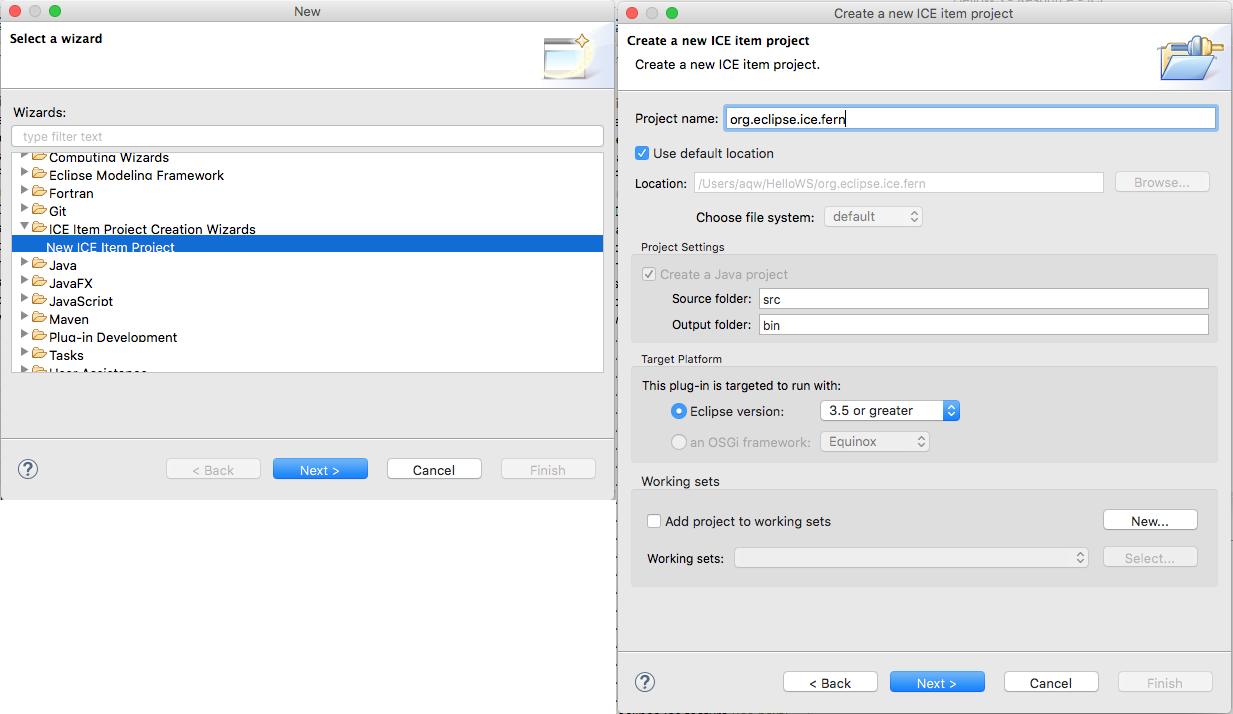
\includegraphics[width=\textwidth]{figures/comb12.png}
\label{fig:comb12}
\end{figure}

To create a new ICE Item project, navigate to \texttt{File $>$ New $>$ Other}
and open the \texttt{ICE Item Creation Wizards} folder and 
select \texttt{ICE Item Creation Wizard}. You will be met with a standard new
project wizard page, in which you can name your project.  We will call ours
\texttt{org.eclipse.ice.fern}. Once you have named your project click the \texttt{Next >} button.
\begin{center} 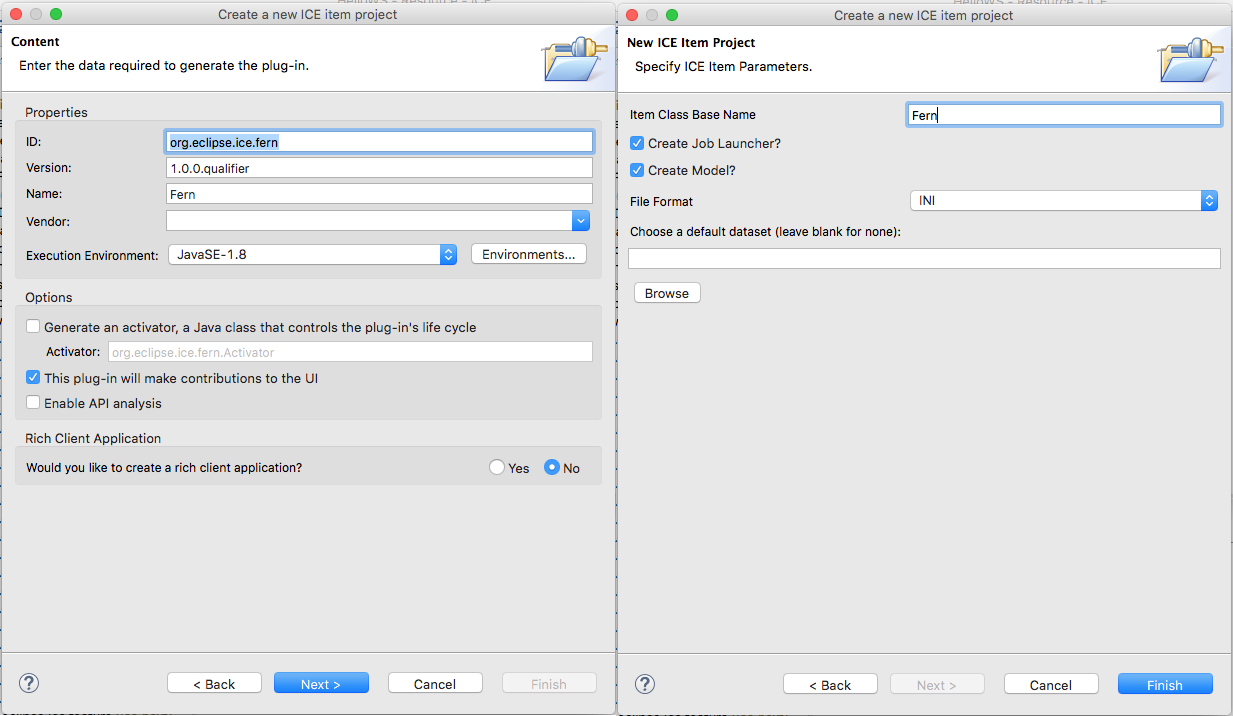
\includegraphics[width=\textwidth]{figures/comb23} \end{center}
Now you are able to customize the plugin-specific portions of the project. 

On this page you need to tell the wizard what you want to use as a base
name for your item classes. We will call this one \texttt{Fern}. Then, we will
specify some information about how the item will handle input data.  Fern uses
the INI file format to specify data, so we will tell our item to use the built-in
functionality for INI files.  To do this select \texttt{INI} from the \texttt{File Format} dropdown.  

When you have entered all of the required information you can
click the \texttt{Finish} button to generate your new ICE Item plugin project.
When the project has finished generating you should be able to explore the code
that has been created.  Within the source directory there will be two packages,
each containing two Java classes:

\begin{itemize} 
    \item \texttt{org.eclipse.ice.fern.launcher} 
    \begin{itemize}
        \item \texttt{FernLauncher.java} 
        \item \texttt{FernLauncherBuilder.java}
    \end{itemize} 
    \item \texttt{org.eclipse.ice.fern.model} 
    \begin{itemize} 
        \item \texttt{FernModel.java} 
        \item \texttt{FernModelBuilder.java}
    \end{itemize} 
\end{itemize}

To add functionality to the project we need to edit
the \texttt{FernLauncher} and \texttt{FernModel} classes.

\section{Adding Functionality to the New Items}

\subsection{The Fern Model}

The \texttt{FernModel} will be responsible for creating and
validating input parameters for FERN, in the form of a new FERN input file.  In
order to make the generated code run there are several pieces of information that need to be changed.  First, we
will need to set up the basic Item idenfification information. This information
is set in the setupItemInfo() method. Modify the outputName to match the
following (or something of your choosing, with a .ini file extenstion).

\begin{lstlisting}[language=Java]
outputName = "fern_config.ini";
\end{lstlisting}

The String for the \emph{setName} method will serve as the display name
for this Item, so set it as \texttt{Fern Model}.
As for the String for \emph{setDescription}, this will also be used on the UI
for the Item, so provide some text like the following: \texttt{This Item constructs input files
for the FERN reaction network solver}. The export string will serve as the name
of the action that the user can select to write the provided data to file. Set
it to something like: \texttt{Export to INI}. You should now have a method that
looks like this:

\begin{lstlisting}[language=Java]
@Override
protected void setupItemInfo() {
	setName("Fern Model");
	setDescription("This Item constructs " +
	    "input files for the FERN reaction " +
	    "network solver"); 
	outputName = "fern_output.ini";   
	exportString = "Export to INI";
	allowedActions.add(0, exportString);
	ioFormat = "INI";
	defaultFileName = "";
}
\end{lstlisting}

The \emph{allowedActions.add()} line ensures that the export string is provided
to ICE as an allowed action, and displayed in the Item Process drop down.

With the identification information configured properly we can begin to
implement the Form for this Fern Model. This is done in the \emph{setupForm()}
method.
The generator has begun the process of implementing this method by instantiating
a Form for you to use, getting a reference to the IOService (which provides
IReader/IWriter realizations), and providing a commented out example of how to
fill out an ICE Form.

For this FERN input model, we want to add the following sections with data
entries: a network section with 
numSpecies, numReactions, numReactionGroups, massTol, fluxFrac, networkFile,
rateFile data entries, an initialConditions section with T9, startTime, endTime,
initialTimeStep, and density, and an output section with a single popFile
data entry.
To achieve this for this Item, we will need to add three
\texttt{DataComponents}, one for the network section, another for the
initialConditions section, and a final one for the outputs section. To each of
those DataComponents we will add appropriate IEntry instances for each of the data entries we have.

Add the following to your setupForm() method: 

\begin{lstlisting}[language=Java]

    // Create the network section
    DataComponent networkComp = new DataComponent();
    networkComp.setName("network");
    networkComp.setDescription("The parameters needed " +
        "to describe the nuclear " +
    	"reaction network"); 
    networkComp.setId(1);
    
    // Create the IEntries we need for this DataComponent
    StringEntry numSpecies = new StringEntry();
    numSpecies.setName("numSpecies");
    numSpecies.setDescription("The number of species to consider");
    numSpecies.setDefaultValue("16");
    
    StringEntry numReactions = new StringEntry();
    numReactions.setName("numReactions");
    numReactions.setDescription("The number of reactions to consider");
    numReactions.setDefaultValue("48");
    
    StringEntry numReactionGrps = new StringEntry();
    numReactionGrps.setName("numReactionsGroups");
    numReactionGrps.setDescription("The number of reaction " + 
    	"groups to consider"); 
    numReactionGrps.setDefaultValue("19");

    StringEntry massTol = new StringEntry();
    massTol.setName("massTol");
    massTol.setDescription("The mass tolerance to consider");
    massTol.setDefaultValue("1e-7");
    
    StringEntry fluxFrac = new StringEntry();
    fluxFrac.setName("fluxFrac");
    fluxFrac.setDescription("The flux fraction to consider");
    fluxFrac.setDefaultValue(".01");
    
    FileEntry networkFile = new FileEntry(".inp");
    networkFile.setProject(project);
    networkFile.setName("networkFile");
    networkFile.setDescription("The network file for this problem");
    
    FileEntry rateFile = new FileEntry(".data");
    rateFile.setProject(project);
    rateFile.setName("rateFile");
    rateFile.setDescription("The rate file for this problem");
    
    networkComp.addEntry(numSpecies);
    networkComp.addEntry(numReactions);
    networkComp.addEntry(numReactionGrps); 
    networkComp.addEntry(massTol);
    networkComp.addEntry(fluxFrac);
    networkComp.addEntry(networkFile);
    networkComp.addEntry(rateFile);
    
    // Create the initial conditions section
    DataComponent initConditionsComp = new DataComponent();
    initConditionsComp.setName("initialConditions");
    initConditionsComp.setId(2);
    initConditionsComp.setDescription("The parameters " +
    	"needed to describe the	initial " + 
    	"conditions for the problem");
    
    StringEntry t9 = new StringEntry();
    t9.setName("T9");
    t9.setDescription("The temperature in Kelvin x 10^9");
    t9.setDefaultValue("7.0");

    StringEntry startTime = new StringEntry();
    startTime.setName("startTime");
    startTime.setDescription("The start time for the simulation.");
    startTime.setDefaultValue("1e-20");

    StringEntry endTime = new StringEntry();
    endTime.setName("endTime");
    endTime.setDescription("The end time for the simulation");
    endTime.setDefaultValue("1e-3");

    StringEntry initialTimeStep = new StringEntry();
    initialTimeStep.setName("initialTimeStep");
    initialTimeStep.setDescription("The initial time step " + 
    	"for the simulation."); 
    initialTimeStep.setDefaultValue("1.2345e-22");

    StringEntry density = new StringEntry();
    density.setName("density");
    density.setDescription("The initial density.");
    density.setDefaultValue("1e8");
    
    initConditionsComp.addEntry(t9);
    initConditionsComp.addEntry(startTime);
    initConditionsComp.addEntry(endTime);
    initConditionsComp.addEntry(initialTimeStep);
    initConditionsComp.addEntry(density);
    
    // Create the outputs section
    DataComponent outputComp = new DataComponent();
    outputComp.setName("output");
    outputComp.setDescription("The parameters needed to output data.");
    outputComp.setId(3);
    
    StringEntry popFile = new StringEntry();
    popFile.setName("popFile");
    popFile.setDescription("The name of the output populations file");
    popFile.setDefaultValue("popFile.csv");
    
    outputComp.addEntry(popFile);
    
    // Add the components to the Form
    form.addComponent(networkComp);    
    form.addComponent(initConditionsComp);
    form.addComponent(outputComp);
    
\end{lstlisting}

Now we have a Form constructed for a typical FERN execution. 

The default generated implementation of the process method is sufficient to be
able to create new Fern INI input files. 

\subsection{Fern Launcher}
The Fern Launcher handles the actual execution of the FERN application. The
generator creates the FernLauncher as a subclass of ICE's JobLauncher, which
provides a large array of features and functionality. As a subclass of
JobLauncher, the FernLauncher enables users to execute Fern locally or remotely.
To do so, we just need to add a small amount of
code that customizes the ICE job launching capabilities for Fern. 

The first bit of code to add to the FernLauncher specifies the name of the
actual Fern executable. In the setupItemInfo() method, set the execCommand to
the following: 
\begin{lstlisting}[language=Java]
execCommand = "${installDir}fern-exec";
\end{lstlisting}
This tells ICE that the Fern executable is called \texttt{fern-exec}, and to
set the overall execution command to it's install path plus the executable name.
The installDir flag will tell ICE to insert the user-specified executable
location (provided through the graphical form editor') into the execCommand,
with a trailing OS-specific path separator. This install directory is
specified through the Hosts Table on the editory. 

We also need to inform the JobLauncher what other files are involved in this
execution. To do that, the JobLauncher provides an addInputType() method. Add
the following to setupForm():
\begin{lstlisting}[language=Java]
addInputType("Network File", "networkFile", 
			"Network File Description", ".inp");
addInputType("Rate File", "rateFile", "
			Rate File Description", ".data");
\end{lstlisting}

And that should be it.
The generator has taken care of everything else for us.
We are now ready to launch ICE with our Fern plugin, and use the Fern Items we
have just created.

\section{Using the New Fern Items}
Now, using these new Items is easy. From the Developer top-level menu, select 
ICE $>$ Launch New Instance. This will display a dialog asking you which new
plugins you'd like to include as part of the new ICE instance. 
\begin{center} 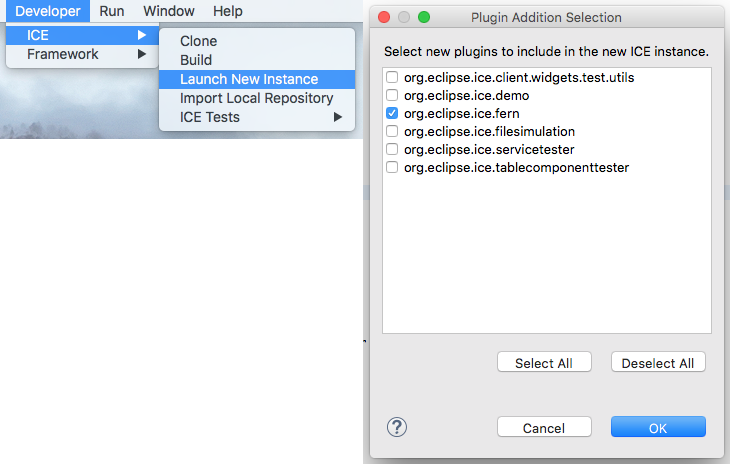
\includegraphics[width=\textwidth]{figures/combdev}
\end{center}
Select \texttt{org.eclipse.ice.fern} and click Ok. This will create and launch a
new instance of ICE that includes your custom Item plugin. 

With a new ICE instance open, close the Welcome view if necessary and go to
\texttt{File $>$ New $>$ Other} and select the Create Item Wizard. 
\begin{center} \includegraphics[width=\textwidth]{figures/creatingFernModelItem}
\end{center}
After selecting the FernModel Item, you will be presented with the view in the
figure below. 
\begin{center} 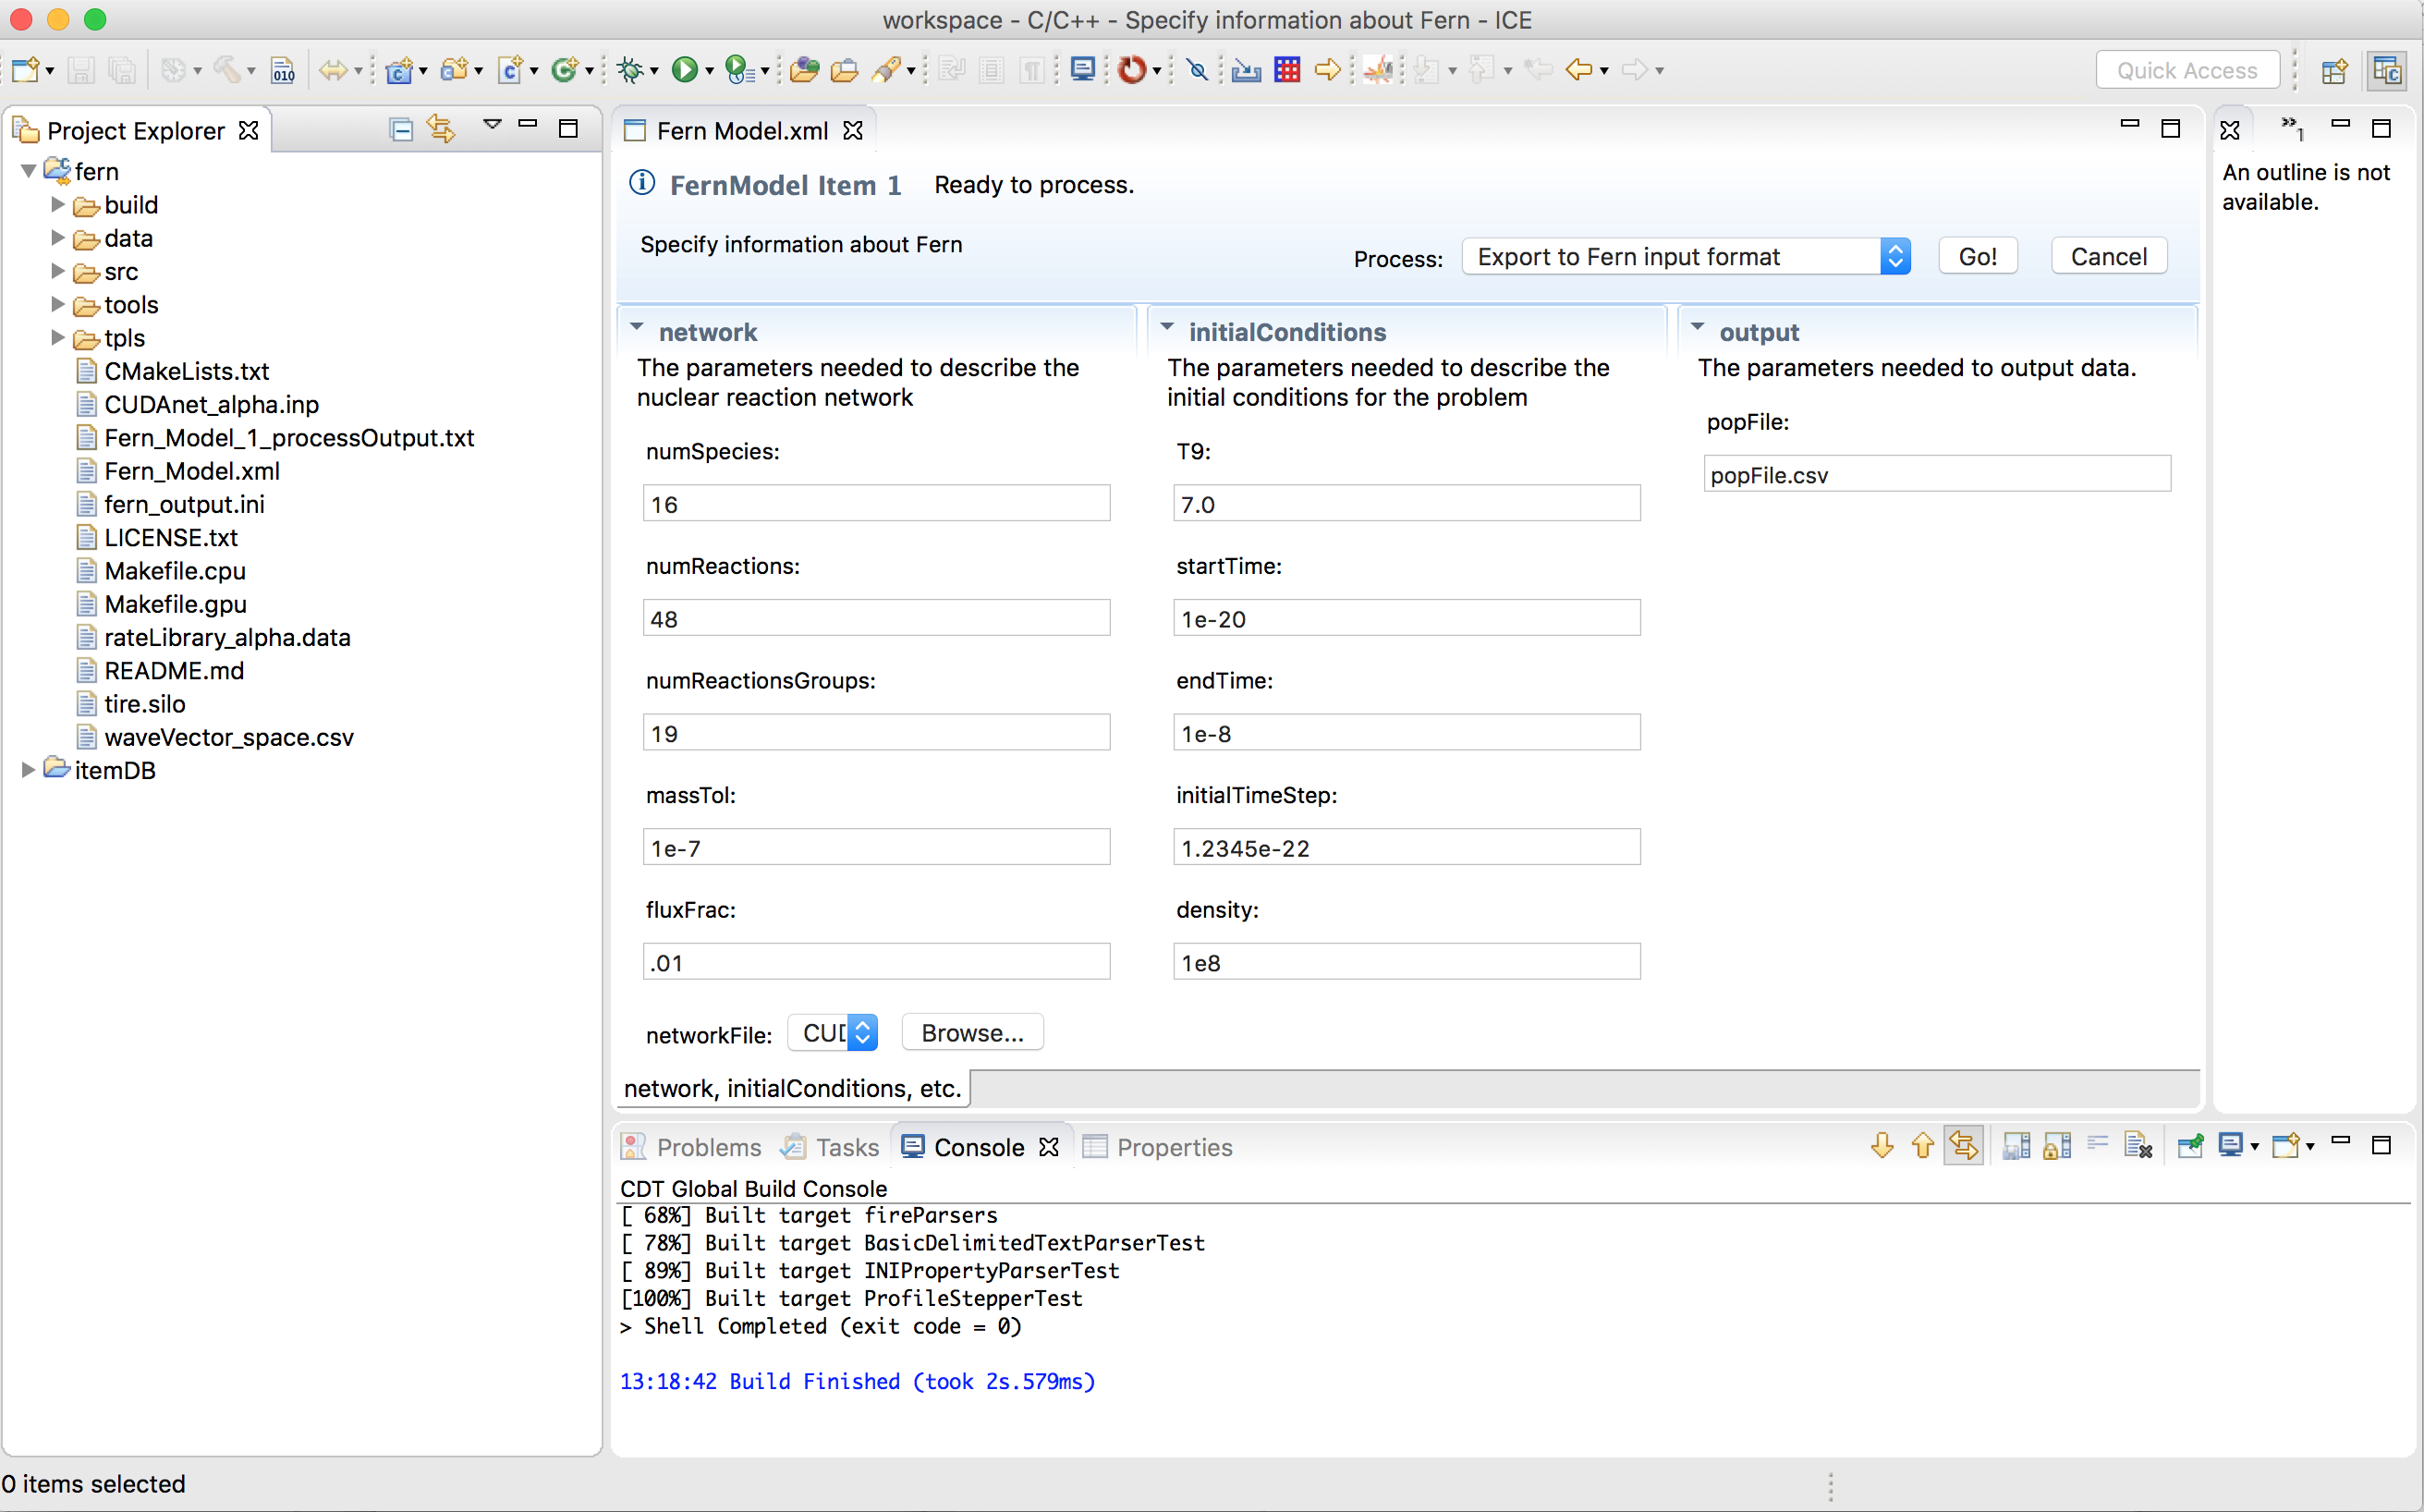
\includegraphics[width=\textwidth]{figures/fernmodelItem}
\end{center}
Here you can modify the various defaults with the values you would like for a
given Fern simulation. Once done, simply save the Item and click Go on the
Export to INI Process. This will execute the process of creating a new INI Fern
input file for use with the Fern Launcher. You can check the result by opening
the fern\_output.ini file, as shown below. 
\begin{center} 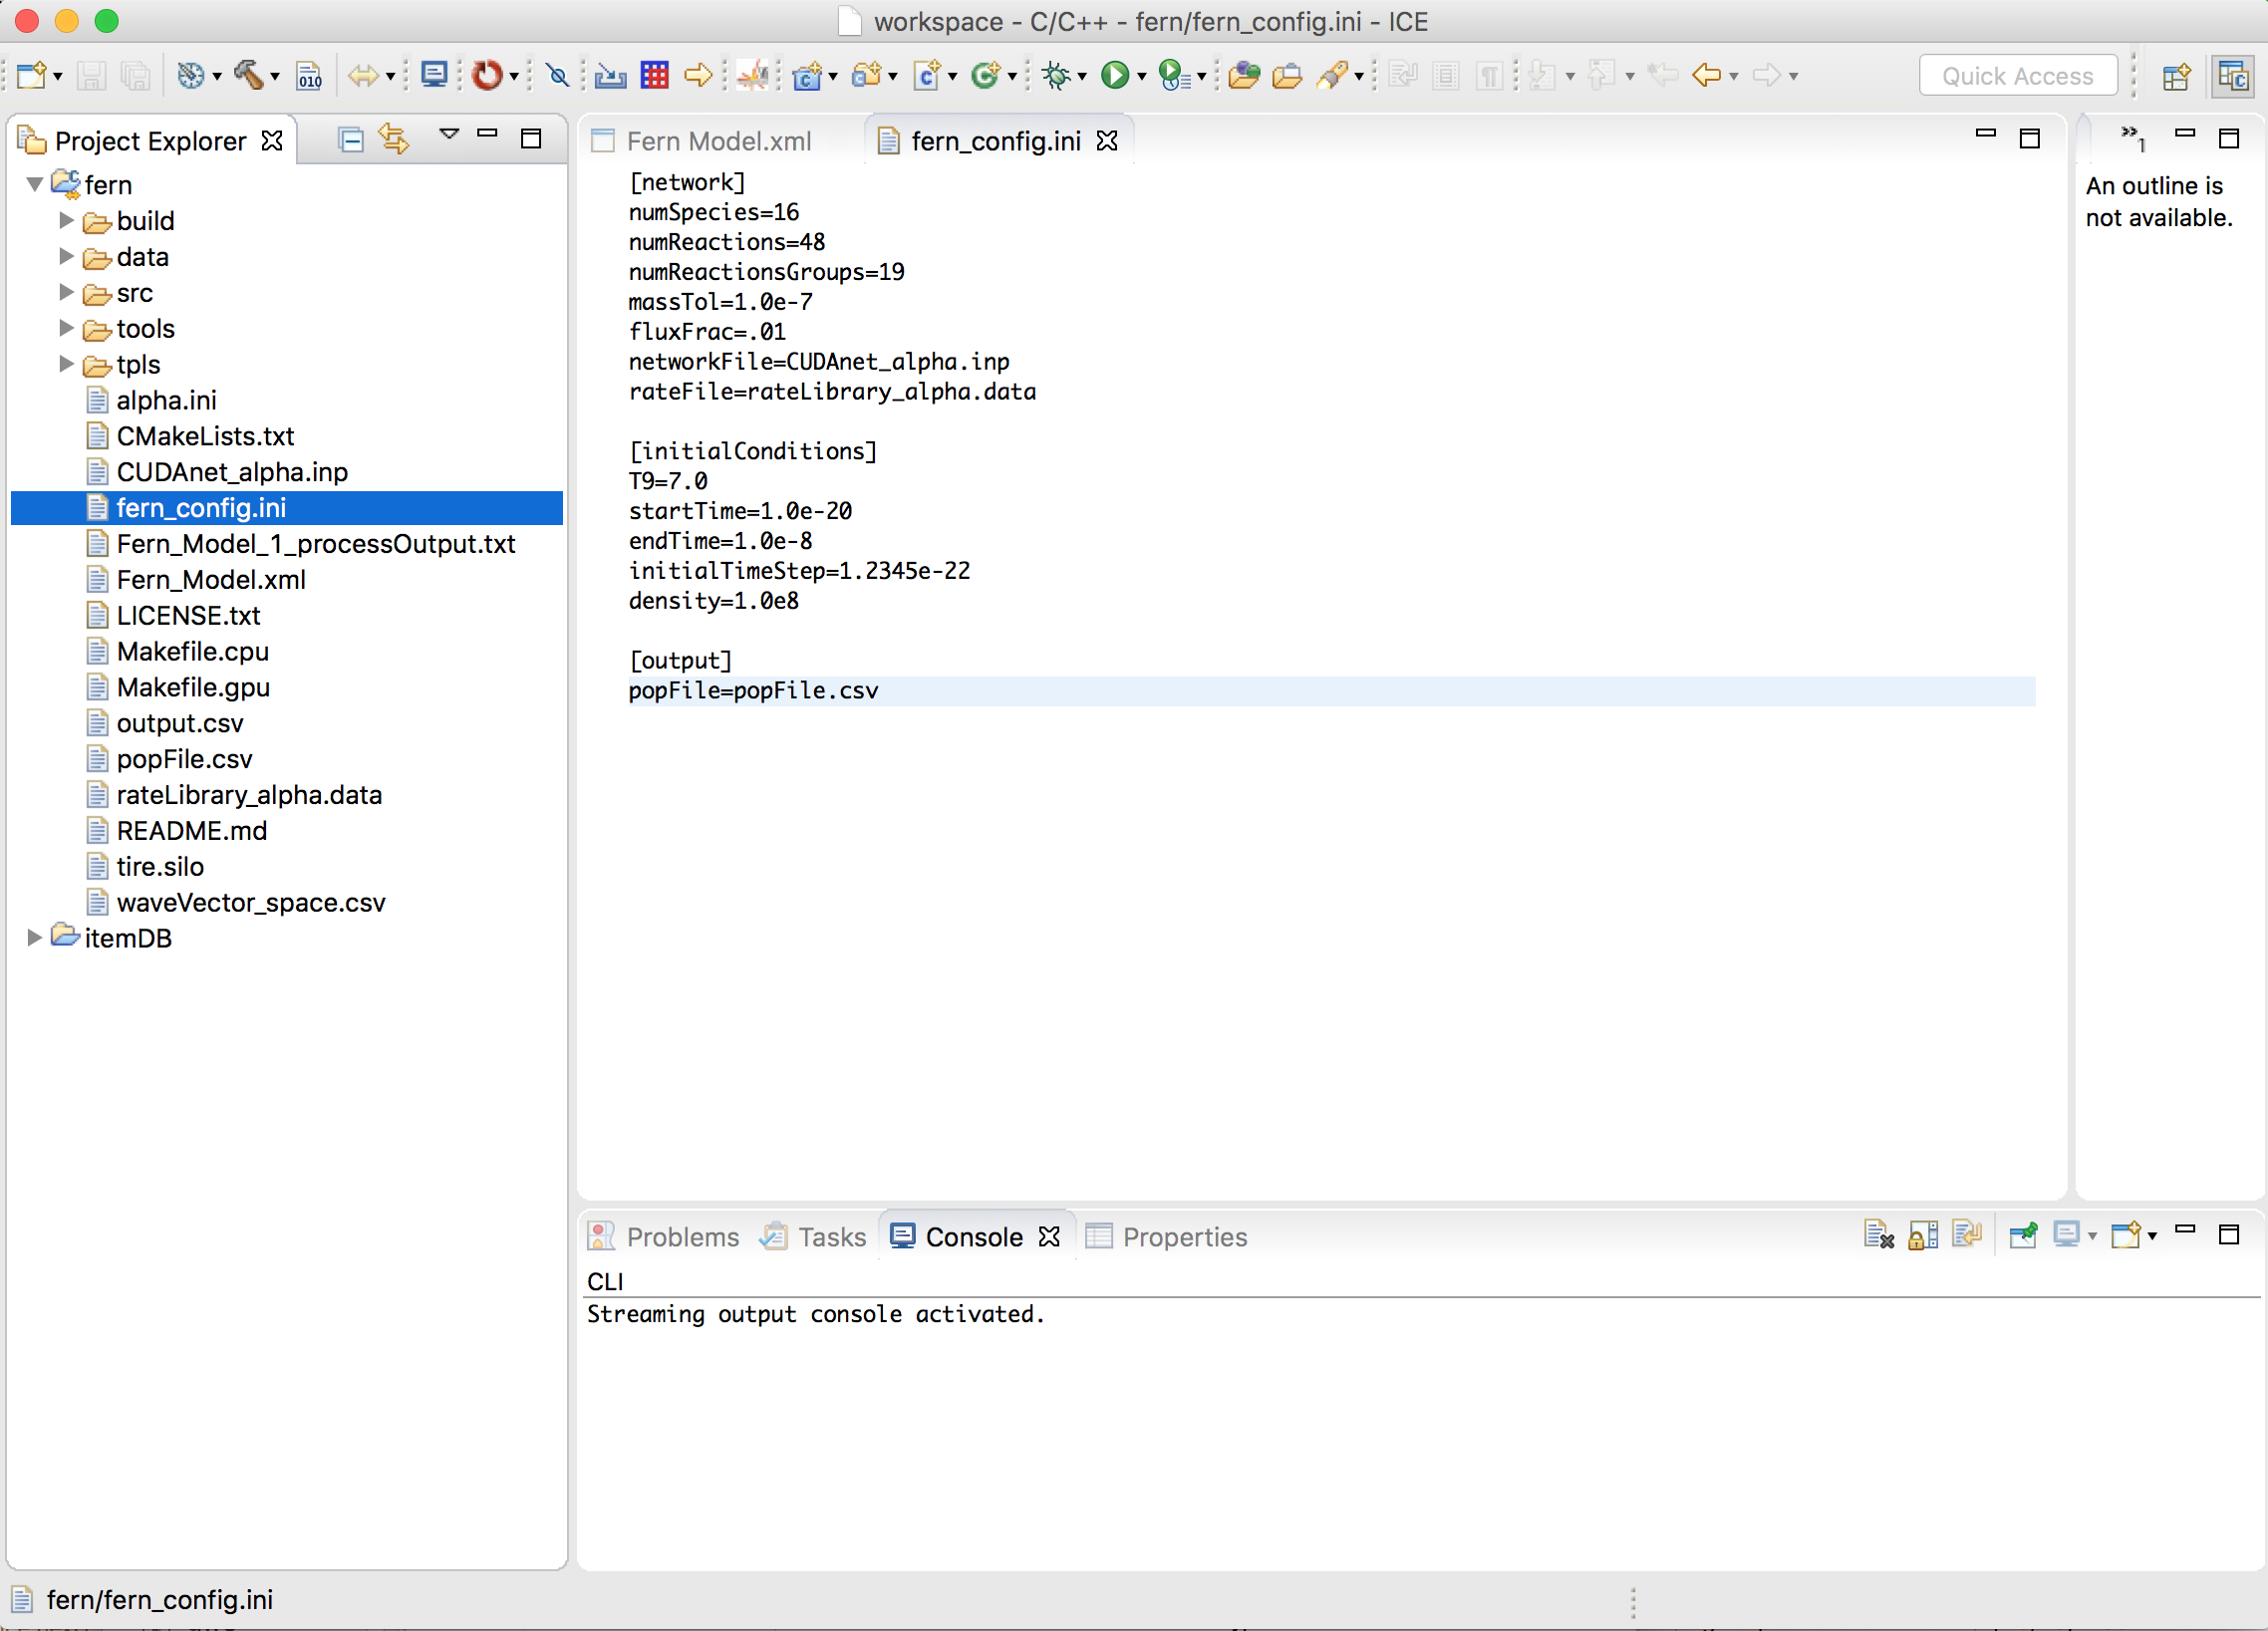
\includegraphics[width=\textwidth]{figures/result}
\end{center}

Now you can similarly create a new Fern Launcher. After creating the Launcher,
you should see a view like below. 
\begin{center} 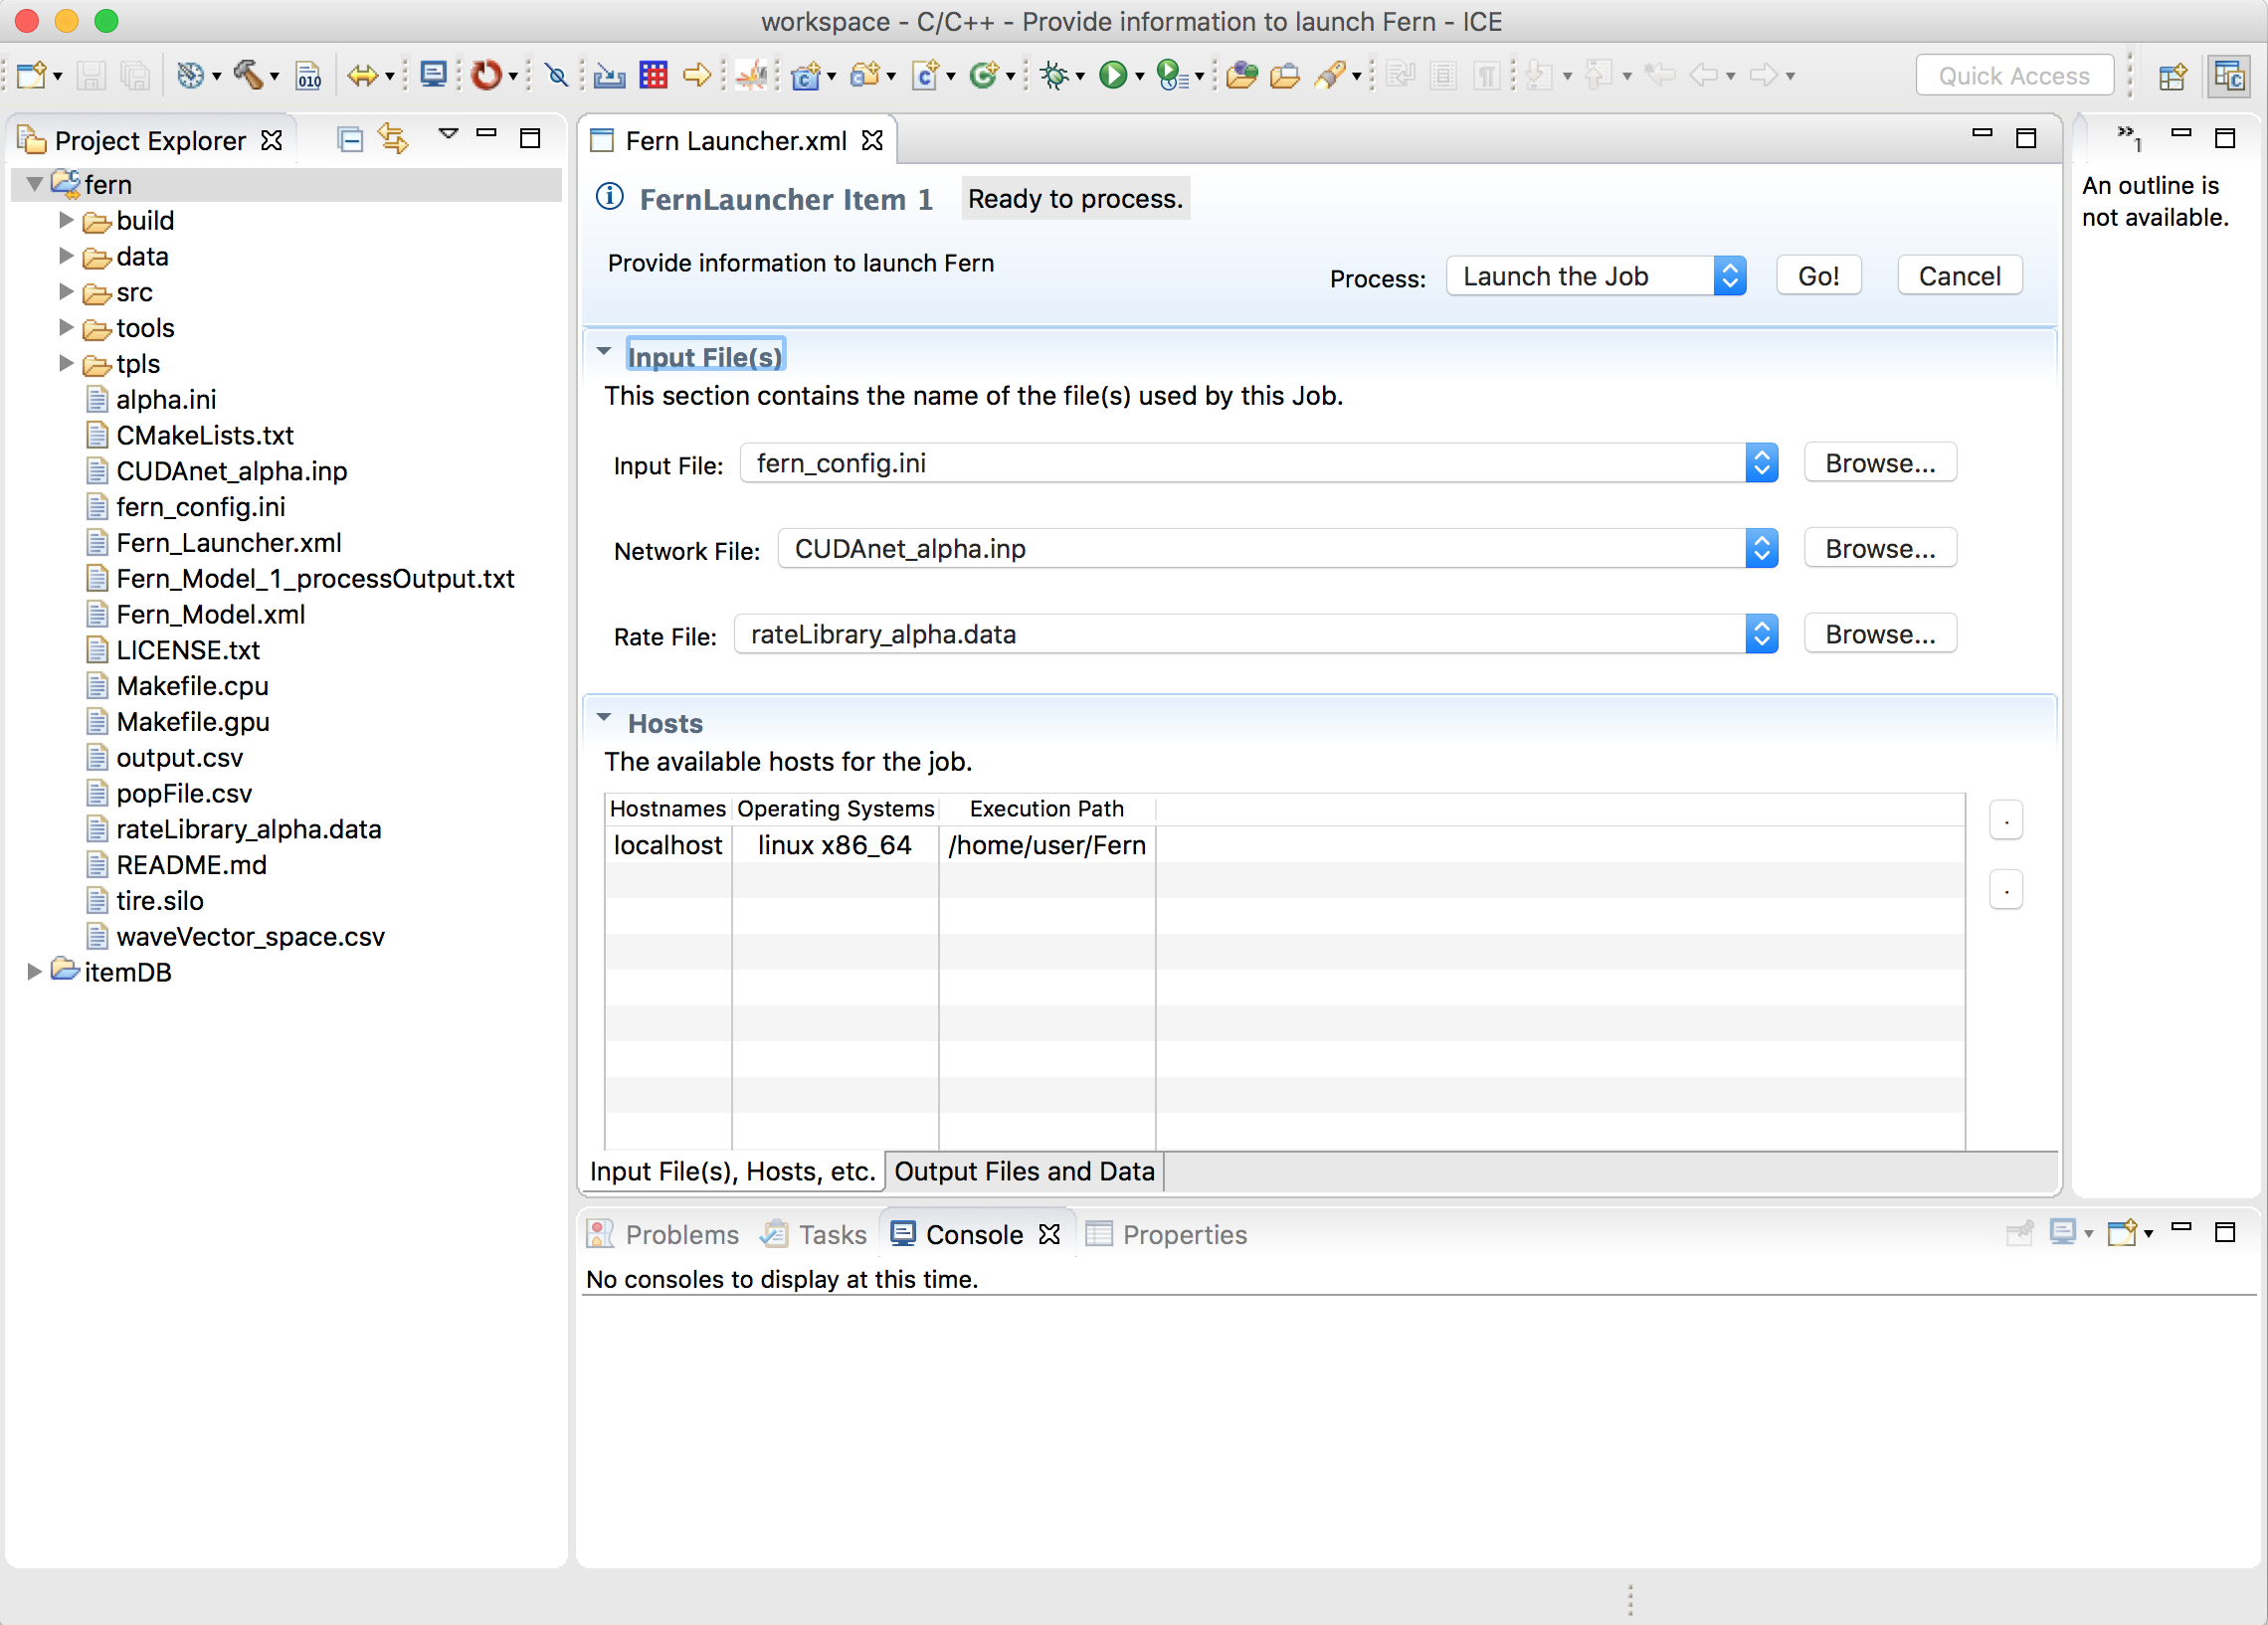
\includegraphics[width=\textwidth]{figures/launcher}
\end{center}
To configure a launch, simply set the correct
input file, along with its dependent network and rate files. 

At this point, if you had Fern built on your local machine, or if you had it
built on some remote host, you could configure that in the Hosts table. ICE
would then execute Fern based on that input. 

After the execution you should see the results in the Console, as shown below.
\begin{center} 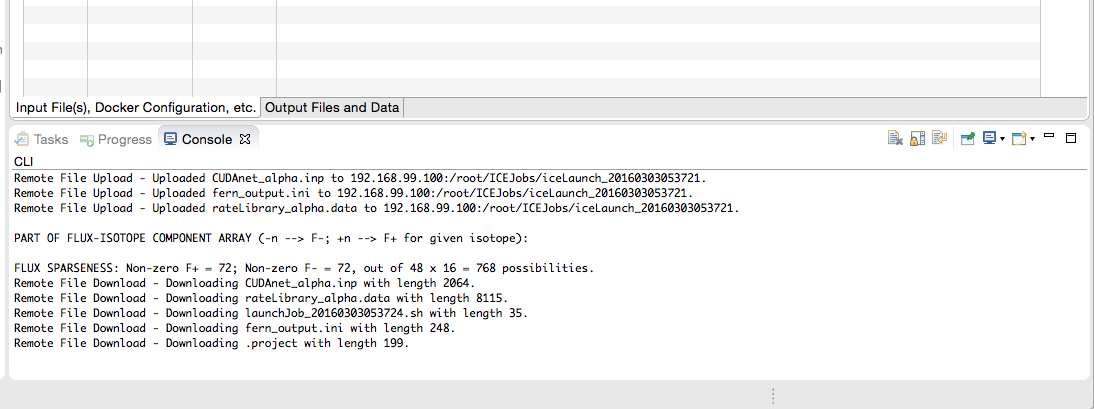
\includegraphics[width=\textwidth]{figures/launcherResult}
\end{center}
The execution should have produced a CSV file with the computed populations. You
can double-click that file to view them graphically in the ICE Plot Editor. 


\chapter{Creating and Using an Application Dashboard}
\graphicspath{{../../newItemGeneration/src/}}
Resource Components are ICE Components which contain a grid of visualization
resources. These resources can display files from a variety of sources,
such as CSV files or VisIt visualizations. Geometry and Mesh editors allow for
editing of shapes or meshes. All three can be added to an Item to offer
visualization of data.

\section{Prerequisites}

You will need access to an installation of VisIt version $2.9.2$. There is a copy of the
software in the VisIt folder of your USB drive. Windows users should open the Windows installer, while users of
other OSs can just copy the appropriate folder onto their machine.

\section{Adding the Components}

We will be adding the visualization components to the model made in the
previous section, so return to your original ICE window, closing the launched
instance. For convenience, you can copy and paste the code from the
XSEDEVisualizationeModel.java in the org.eclipse.ice.demo.visualization.model
package. Its location can be seen in figure \ref{fig:demostructure}.

\begin{figure}[!h]
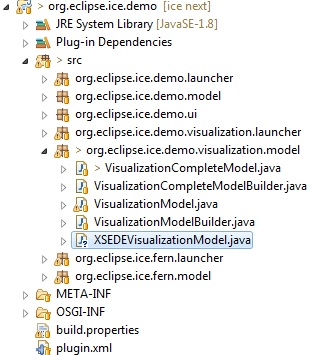
\includegraphics[width=200]{images/XSEDEDemoPackageStructure}
\centering
\caption{The package structure for org.eclipe.ice.demo bundle}
\label{fig:demostructure}
\end{figure}

First, copy and paste the following example code into the end of your Item's
setupForm() method. You can also find this code in
XSEDEVisualizationModel's setupForm() method, but be sure to note the
comments specifying where to begin and end copying. 

{\small
\begin{verbatim}
		//Create the resource component
		ResourceComponent resourceComponent = new ResourceComponent();

		//Set the component's data members
		resourceComponent.setName("Resource Component");
		resourceComponent.setDescription("Results");
		resourceComponent.setId(1);

		//Declare the files and resources
		VizResource csvResource = null;
		VizResource visItResource = null;
		IFile csvFile = null;
		IFile visItFile = null;


		//If the file was found, create the CSV resource and add it to the component
		try{
			
			//Open the files
			csvFile = ResourcesPlugin.getWorkspace().getRoot().getProject("itemDB").getFile("fib8.csv");
			visItFile = ResourcesPlugin.getWorkspace().getRoot().getProject("itemDB").getFile("tire.silo");
			
			//If the file was found, create the CSV resource and add it to the component.
			if(csvFile.exists()){
				csvResource = new 
		                    VizResource(csvFile.getLocation()
		                    .toFile());
		    	resourceComponent.addResource(csvResource);
			}
				        
			//If the file was found, create the VisIt resource and add it to 
			//the component
			if(visItFile.exists()){
				visItResource = new 
		                    VizResource(visItFile.getLocation()
		                    .toFile());
				resourceComponent.addResource(visItResource);
			}
		}
		catch(IOException e){
			e.printStackTrace();
		}

		//Create the geometry component
		ShapeController geometryRoot = new ShapeController(new
		    Shape(), new BasicView());
		GeometryComponent geometryComponent = new 
		    GeometryComponent();
		geometryComponent.setGeometry(geometryRoot);
		geometryComponent.setName("Geometry Editor");

		//Create mesh component
		MeshComponent meshComponent = new MeshComponent();
		meshComponent.setName("Mesh Editor");

		//Add the components to the form
		form.addComponent(resourceComponent);
		form.addComponent(geometryComponent);
		form.addComponent(meshComponent);	
		
		// Set the context on the Form
		form.setContext("visualization");
\end{verbatim} 
}

This will cause errors in your file. To resolve them, first open the MANIFEST.MF
file in your project's META-INF folder, switch to the \texttt{Dependencies} tab,
and click the \texttt{Add} button under the \texttt{Imported Packages} section,
both highlightted in figure \ref{fig:manifest}. Select
\texttt{org.eclipse.eavp.viz.datastructures}, press \texttt{OK}, and save the
file. You can then return to your model file, hover over the underlined code
for each of the errors until a menu pops up, and select the option to add a
package to the imported packages, as seen in figure \ref{fig:hover}. Repeat the process, this time choosing the option to import the class. Save the file when the hover menu no longer appears over
errors.

\begin{figure}[!h]
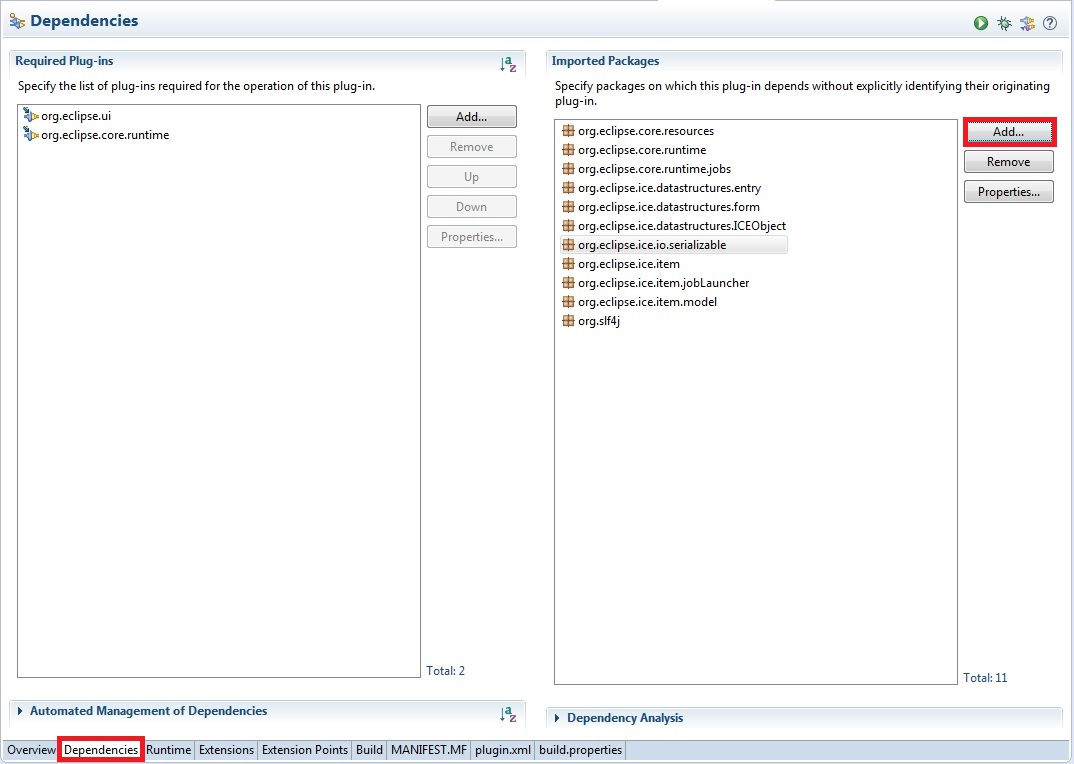
\includegraphics[width=\textwidth]{images/ManifestDependencies}
\centering
\caption{The Manifest dependencies view}
\label{fig:manifest}
\end{figure}

\begin{figure}[!h]
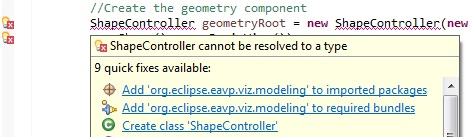
\includegraphics[width=\textwidth]{images/ErrorHoverMenu}
\centering
\caption{The menu displayed when hovering the mouse over code with an error.}
\label{fig:hover}
\end{figure}

This code will add a Resource Component, Geometry Component, and Mesh Component
to your Item and load tire.silo into the Resource Component. When done, launch
ICE again, using \texttt{Developer} $rightarrow$ \texttt{ICE} $rightarrow$
\texttt{Launch New Instance}.

\section{Using the Resource Component}

ICE uses an instance of VisIt, a visualization code from Lawrence Livermore
National Laboratory, running in another process for visualization. ICE can also
use ParaView, but this tutorial will only cover VisIt, as the processes for
conencting to ParaView and using a ParaView Plot Editor are largely similiar to
those for VisIt.

\subsection{Establishing a VisIt Connection}

In order to visualize resources containing VisIt files, ICE must be connected to
a running VisIt installation. To set up this connection, select \texttt{Windows}
$\rightarrow$ \texttt{Preferences...} in ICE's menu bar. (On Mac OS X,
\texttt{Preferences} is instead located under \texttt{ICE} in the menu
bar.)

\begin{figure}[!h]
\includegraphics[width=12cm]{images/ICEPreferences}
\centering
\caption{The ICE \texttt{Preferences Menu} for Windows and Linux. It will be
located under \texttt{ICE} instead of \texttt{Window} on Mac.}
\label{fig:icepreferences}
\end{figure}


Select \texttt{Visualization} $\rightarrow$ \texttt{VisIt} in the tree on the
left side of the \texttt{Preferences} window.

\begin{figure}[!h]
\includegraphics[width=12cm]{images/VisualizationPreferences}
\centering
\caption{The \texttt{VisIt} preferences page in the \texttt{Preferences}
dialog. The hilighted button will add a row for a new connection to the table.}
\label{fig:visualizationpreferences}
\end{figure}


Press the button with a "+" symbol in the upper right of the
\texttt{Preferences Menu} (highlighted in Figure
\ref{fig:visualizationpreferences}) to add a new row to the table.
Click on the \texttt{Path} cell of the new row and put the path of your installation of VisIt.

For example, on \texttt{Windows}, if assuming a username of "username", and
VisIt was installed in the default location, the path will be:

\texttt{C:\textbackslash Users\textbackslash
username\textbackslash AppData\textbackslash Local\textbackslash
Programs\textbackslash LLNL\textbackslash VisIt 2.9.2.}

On \texttt{Linux}, the path will be based on where you extracted the 
visit2\_9\_2.linux-x86 folder, ending with /visit2\_9\_2.linux-x86\_64. If
you unzipped it to the desktop, it will be:
 
\texttt{/home/username/Desktop/visit2\_9\_2.linux-x86\_64}

On \texttt{Mac OS}, the path will be based on the location you put the Visit
application. If placed in the Applications folder it will be

\texttt{/Applications}

Press \texttt{Apply}, then \texttt{OK}, both in the lower right hand corner of
the \texttt{Preferences Menu}.
ICE will now open and connect to this VisIt installation each time ICE is opened.

\subsection{Opening Your Item}
Before opening your new Item, select the itemDB folder in the \texttt{Project
Explorer} and press the import button, highlighted below.

\begin{figure}[!h]
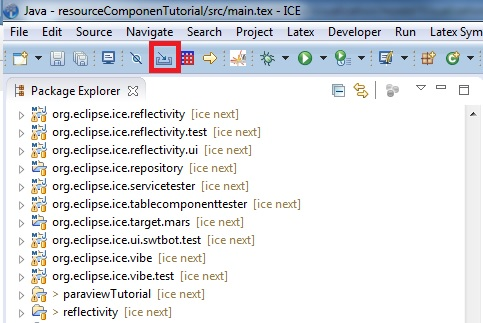
\includegraphics[width=12cm]{images/ImportButton}
\centering
\caption{ICE's \texttt{import} button.}
\label{fig:importbutton}
\end{figure}

Select the files you want to visualize and click OK. For the tutorial,
this should be the tire.silo file from the Fern synchronized project directory.
You should now see the file within the itemDB folder.

Select \texttt{File} $\rightarrow$ \texttt{New} $\rightarrow$
\texttt{Other\ldots} from the toolbar.
In the new dialog, select the \texttt{Create Item Wizard} and hit \texttt{Next}.
Then select \texttt{Visualization Model} and press \texttt{Finish}. You can also select the
\texttt{Visualization Model (Pre-completed)} if you skipped the first part of
the tutorial.

Finally, switch to the ICE Perspective to ensure that the necessary Views will
be open. To do this, click the \texttt{Open Perspective} button in the upper right
of the workbench screen.

\begin{figure}[!h]
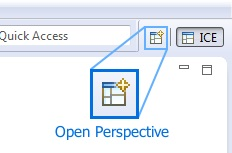
\includegraphics{images/ICE_OpenPerspective}
\centering
\caption{ICE's \texttt{Open Perspective} button.}
\label{fig:openpersepctive}
\end{figure}

In the dialog, select \texttt{ICE} and press {OK}.

\subsection{Managing the Resources}

Your Item should look like this when it loads.

\begin{figure}[!h]
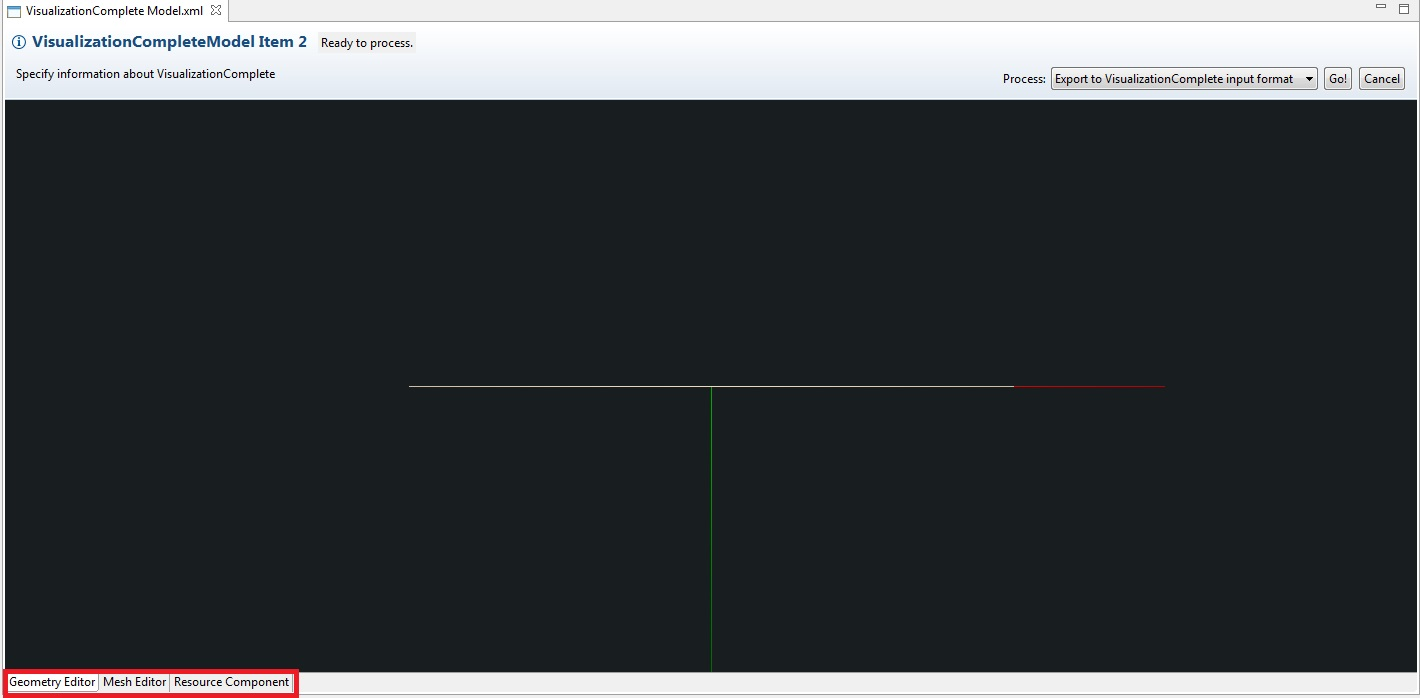
\includegraphics[width=12cm]{images/ItemTabs}
\centering
\caption{The \texttt{Visualization Model} after it is initially opened.
Hilighted in the lower left are the tabs for the three components, the
\texttt{Geometry Editor}, the \texttt{Mesh Editor}, and the \texttt{Resource
Component}.}
\label{fig:itemtabs}
\end{figure}

In the lower left of the \texttt{Visualization Model} are three tabs, hilighted
in Figure \ref{fig:itemtabs}.
Switch to the \texttt{Resource Component} tab in your Item and to the
\texttt{Resources} tab on the left, as shown below.

\begin{figure}[!h]
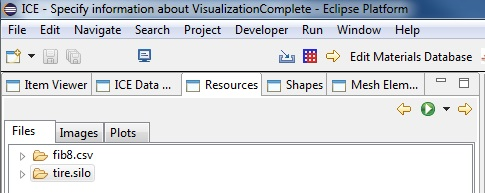
\includegraphics[width=12cm]{images/ResourcesTab}
\centering
\caption{The \texttt{ICE Perspective}'s \texttt{Resources} tab.}
\label{fig:resourcestab}
\end{figure}

Double click on the file named tire.silo to load it into the Resource
Component.

At the top left of the \texttt{Visualization Model} will be controls for the
component's layout.

\begin{figure}[!h]
\includegraphics{images/ResourceComponentControls}
\centering
\caption{The layout controls for the \texttt{Resource Component}.}
\label{fig:resourcecomponentcontrols}
\end{figure}

The \texttt{Clear} button will close all plots in the component. The other two
controls will allow you to specify the number of rows and columns in the grid.
Be careful when reducing them, as any plots which no longer fit in the grid will
be closed.

If you hover over a plot, a button will appear in its upper left hand corner.
Clicking it will close that plot. 

\begin{figure}[!h]
\includegraphics[width=12cm]{images/ClosePlotButton}
\centering
\caption{The X button in the upper left will close the plot.}
\label{fig:closeplotbutton}
\end{figure}

\subsection{Interacting with VisIt Plots}

\begin{figure}[!h]
\includegraphics[width=12cm]{images/VisItPlot}
\centering
\caption{An example of a file open in VisIt displayed in a \texttt{Plot
Editor}.}
\label{fig:visitplot}
\end{figure}

A VisIt plot will contain a 3D visualization of some model. You can click and
drag within the plot to rotate the image and zoom by scrolling your mouse wheel.
Right clicking in the plot will open a context menu, providing options for how
the model will be displayed.

At the bottom of the plot will be a series of controls for animation. If your
plot does not have time series data, they will be greyed out. 

\begin{figure}[!h]
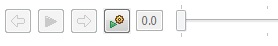
\includegraphics[width=8cm]{images/TimeSliderWidget} 
\centering
\caption{The \texttt{Plot Editor}'s animation controls.}
\label{fig:timesliderwidget}
\end{figure}

The plot can be set to display an arbitrary time step by either dragging the
slider or by typing a time into the box to its left.

\subsection{Editing 3D Structures}

ICE also contains capabilities to render graphics with the Geometry Editor and
Mesh Editor. Programatically populating these editors with custom input is
beyond the scope of this tutorial. However, what follows will be a brief
overview of the editors' functionality.

\subsubsection{The Geometry Editor}

Now switch to the \texttt{Geometry Editor} tab in you the \texttt{Visualization
Model} and the \texttt{Shapes} tab on the left.

Clicking the \texttt{Add Primitives} button will display a drop down of
primitive shapes which can be added to the scene.

\begin{figure}[!h]
\includegraphics[width=12cm]{images/AddPrimitiveShape}
\centering
\caption{The \texttt{Add Primitives} button displays a menu of shapes to add.}
\label{fig:addprimitiveshape}
\end{figure}

Complex shapes can similarly be added using the \texttt{Add Complex} button.

\begin{figure}[!h]
\includegraphics[width=12cm]{images/AddComplexShape}
\centering
\caption{The \texttt{Add Complex} button can add a Union of shapes.}
\label{fig:addcomplexshape}
\end{figure}

Primitive shapes can be added under complex shapes by selecting anything beneath
the desired parent complex shape before adding the new primitive.

\begin{figure}[!h]
\includegraphics[width=12cm]{images/ComplexShapeTree}
\centering
\caption{An example of a constructive solid geometry tree in the
\texttt{Shapes} tab. Adding shapes with the highlighted leaf selected will
cause them to become children of Union 1.}
\label{fig:complexshapetree}
\end{figure}

The three other buttons are responsible for creating copies of or removing
selected shapes from the tree. 

The Transformation View, in the lower left of the workbench screen, has spaces
to set the rotation, scale, and translation of a selected object.

\begin{figure}[!h]
\includegraphics[width=12cm]{images/TransformationView}
\centering
\caption{The \texttt{Transformation View}.}
\label{fig:transformationview}
\end{figure}

\subsubsection{The Mesh Editor}

Now switch to the \texttt{Mesh Editor} tab in your Item and \texttt{Mesh
Elements} tab on your left.

Clicking within the grid will create a vertex, until the fourth completes the
polygon.

\begin{figure}[!h]
\includegraphics[width=12cm]{images/AddPolygon}
\centering
\caption{A new polygon, colored green because the user has not yet permanently
added it to the mesh.}
\label{fig:addpolygon}
\end{figure}

Click again to make the polygon permanent, signified by turning purple, or hit
\texttt{Esc} to cancel.

\begin{figure}[!h]
\includegraphics[width=12cm]{images/NewPolygon}
\centering
\caption{The polygon turns purple after clicking, showing that it has been
finished.}
\label{fig:newpolygon}
\end{figure}

The \texttt{Mode} button in the top left allows you to switch between
\texttt{Add Elements} mode, used previously, and \texttt{Edit Elements} mode.

\begin{figure}[!h]
\includegraphics[width=8cm]{images/EditMode}
\centering
\caption{The \texttt{Mode} button allows switching between \texttt{Edit
Elements} mode and \texttt{Add Elements} mode.}
\label{fig:editmode}
\end{figure}

In edit mode, you can click a vertex (or vertices) to select them. 

\begin{figure}[!h]
\includegraphics[width=12cm]{images/SelectedVertex}
\centering
\caption{A selected vertex will turn blue.}
\label{fig:selectedvertex}
\end{figure}

You can click and drag a vertex to move all selected vertices around the grid.

\section{Further Reading}

This tutorial has only given a brief overview of the ways in which you can use
ICE's visualization tools. For more detailed information, look under the
\texttt{docs} folder in the ICE repository. The visualization folder contains a
tutorial on the CSV and VisIt plots, while the geometryEditor and meshEditor
folders have tutorials on the geometry and mesh editors, respectively. 
\section{Using the Application Dashboard} 

In order to use the functionality you've added to ICE, it is necessary to start
a new \textit{instance} of ICE, called the \textit{runtime} instance. This will
be a completely new copy of ICE that has your new plugins activated. This new
instance is how you and your users will typically interact with your
application. Once you are satisfied with the functionality you have added, you
can create a new \texttt{runtime application} that can be deployed to users.
Creating runtime applications is beyond the scope of this tutorial.

\subsection{Launching a New ICE Instance}

From the \texttt{Developer} top-level menu, select \texttt{ICE $\rightarrow$ Launch New Instance}. This will display a
dialog asking you which new plugins you'd like to include as part of the new ICE instance. 
\begin{center} 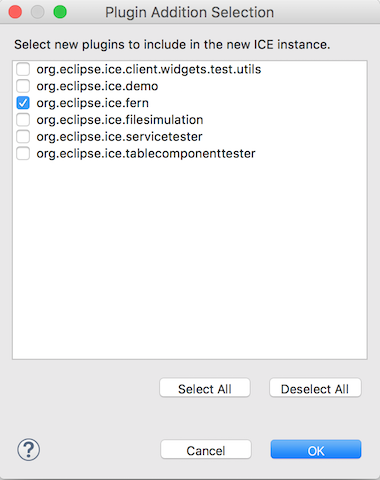
\includegraphics{figures/pluginDialog}
\end{center}
Select \texttt{org.eclipse.ice.fern} (or whatever name you chose for your
plugins) and click \texttt{OK}.
This will create and launch a new instance of ICE that includes your custom
plugins.

\subsection{Importing a Project}

This section will show you how to import existing FERN application source code
and executables into the ICE instance so that you can use it with the dashboard you
have just created. The steps are as follows:

\begin{enumerate}
\item With a new ICE instance open, close the Welcome view if necessary
\item Go to \texttt{Package Explorer} view, right click and select \texttt{New
$\rightarrow$ Synchronized C/C++ Project}

\begin{center} 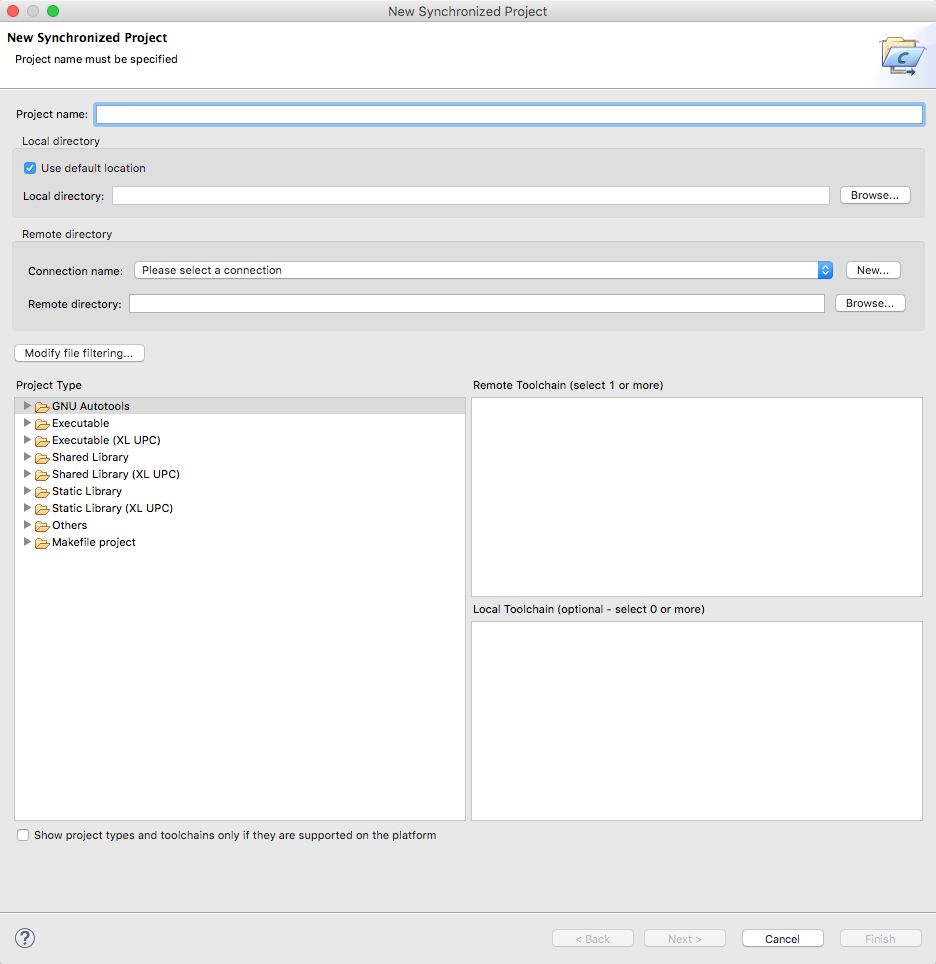
\includegraphics[width=\textwidth]{figures/newSyncWizard}
\end{center}

\item Enter \texttt{fern} for the \texttt{Project name:}
\item Click the \texttt{New\ldots} button next to the \texttt{Please select a
connection} dropdown

\begin{center} 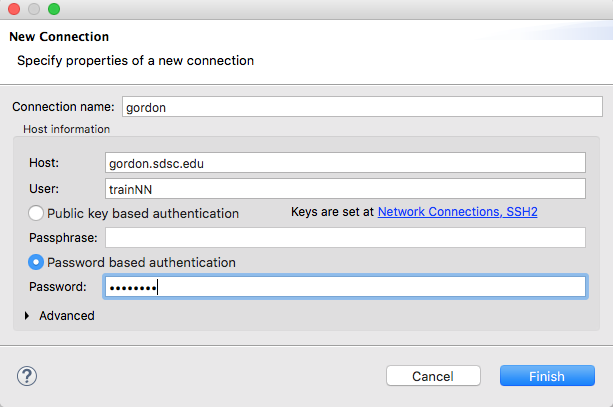
\includegraphics[width=200]{figures/newConnectionDialog}
\end{center}

\item Enter \texttt{gordon} for the \texttt{Connection name}
\item Enter \texttt{gordon.sdsc.edu} for the \texttt{Host}
\item Enter your training username for the \texttt{User}
\item Click on the \texttt{Password based authentication} button
\item Enter the training account password
\item Click \texttt{Finish}
\item Click on the \texttt{Browse\ldots} button

\begin{center} 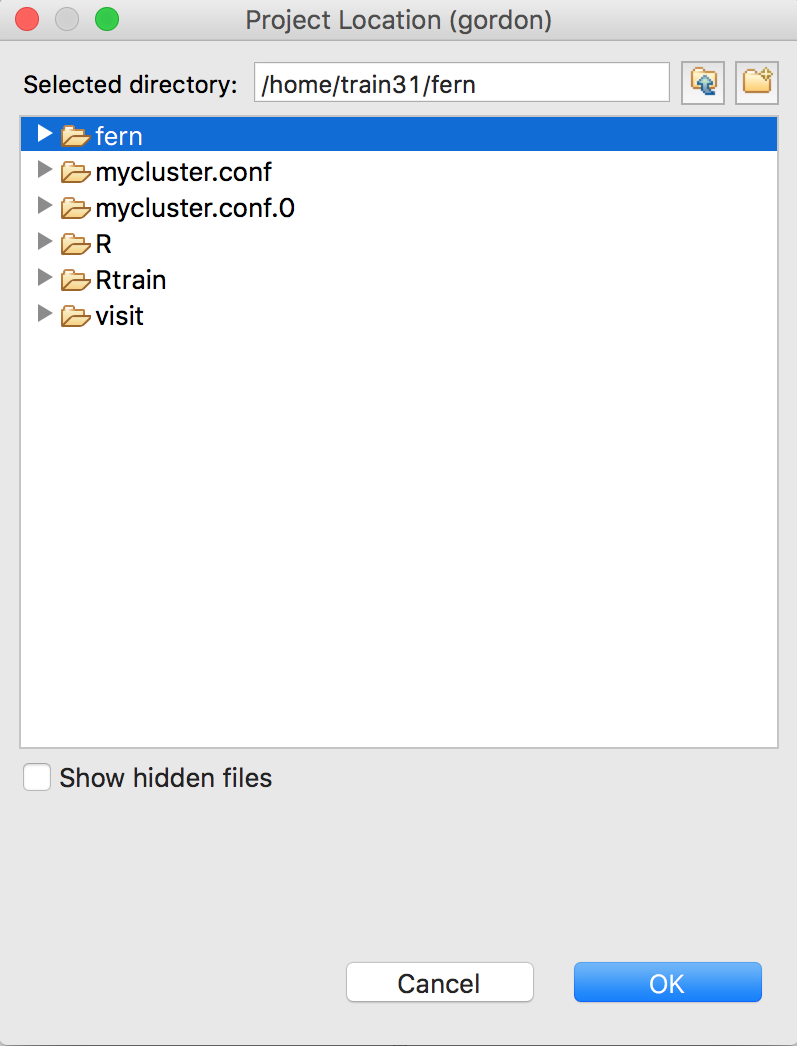
\includegraphics[width=150]{figures/dirBrowser}
\end{center}

\item Select \texttt{fern} from the directory browser and press \texttt{OK}

\begin{center} 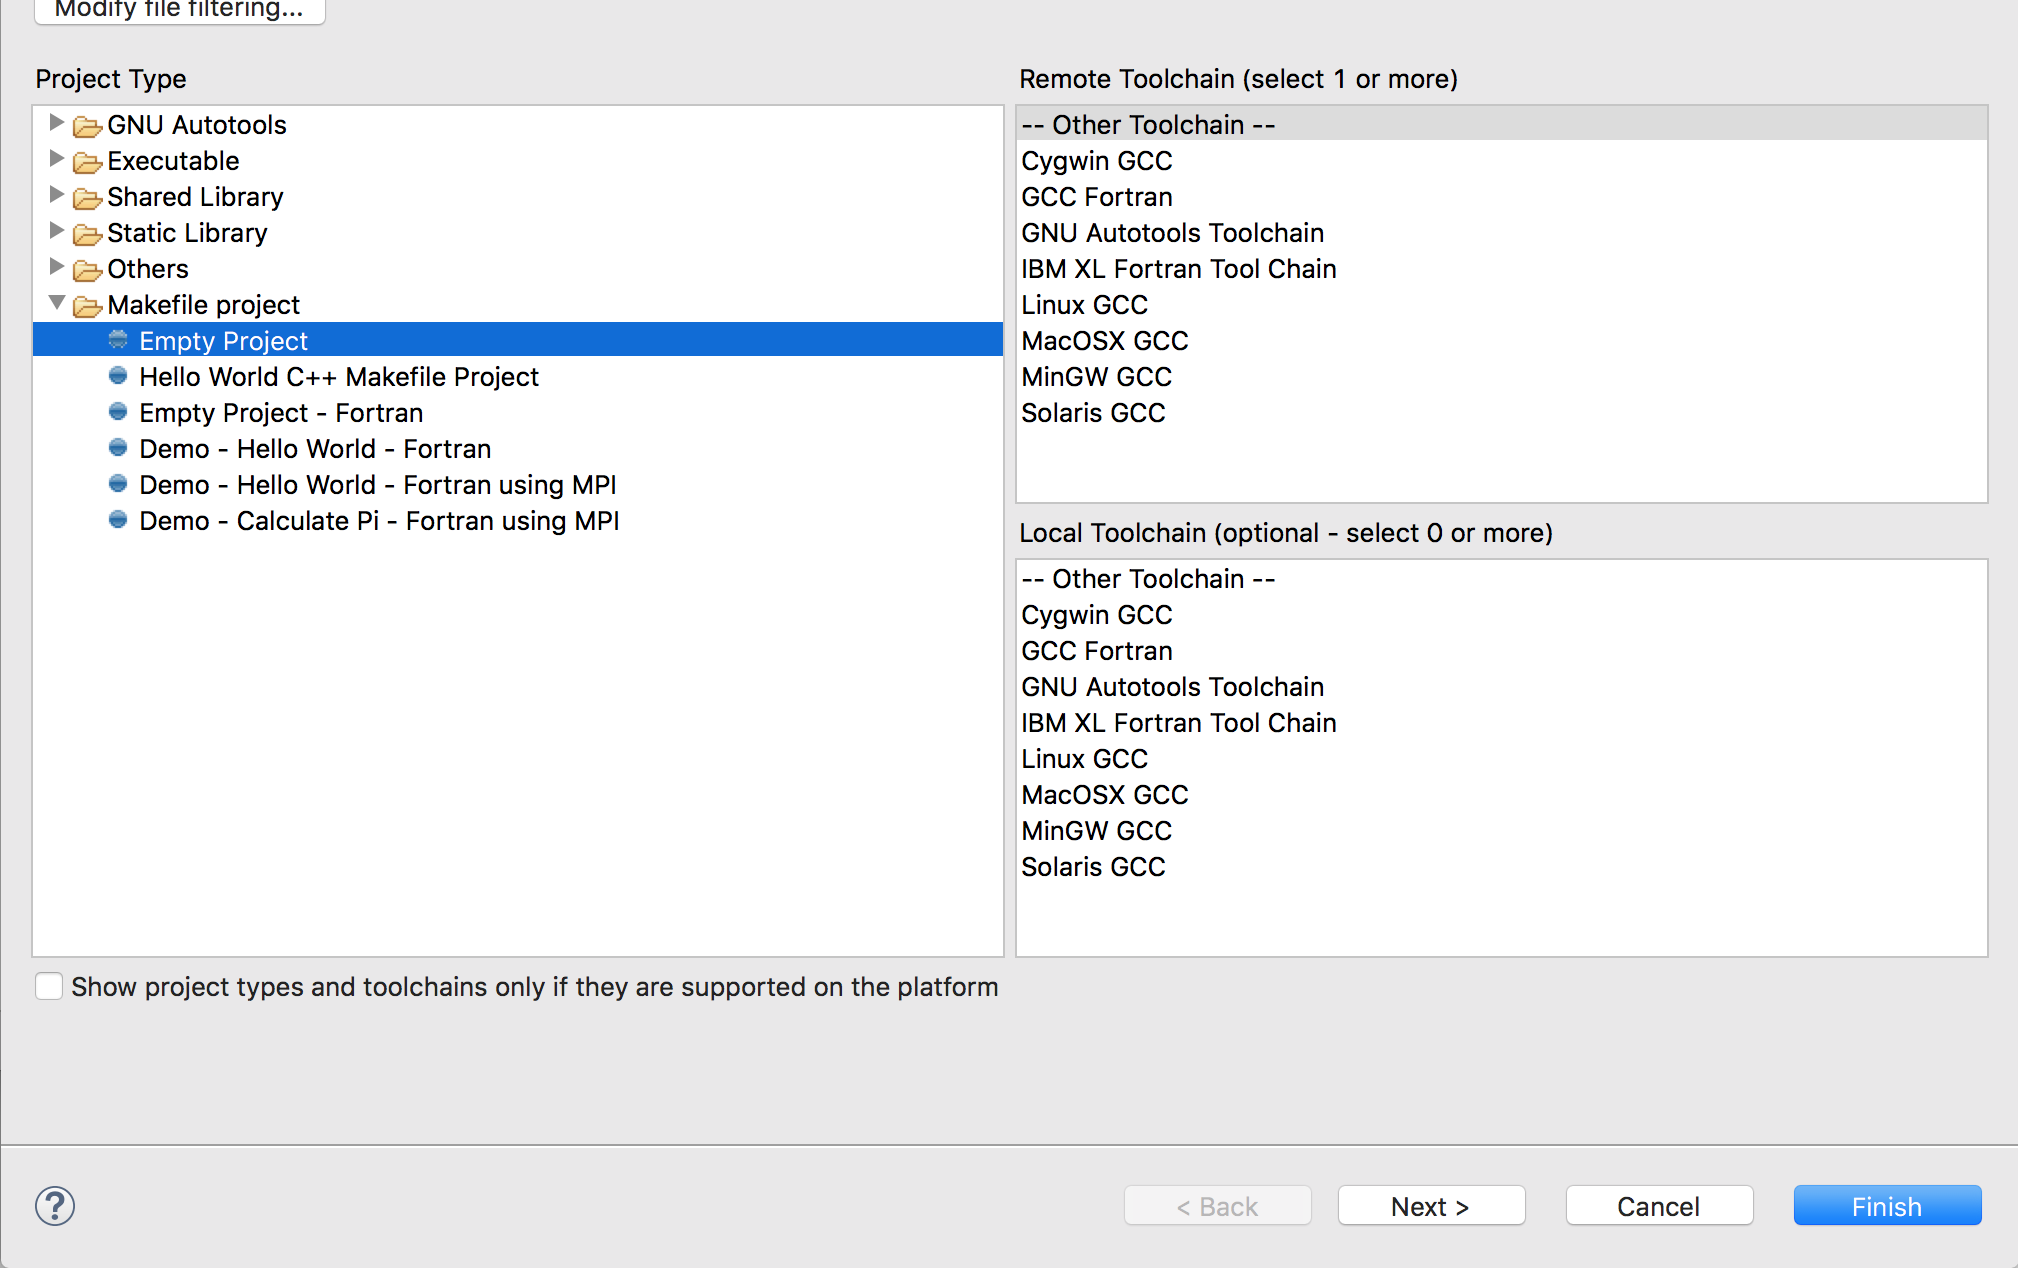
\includegraphics[width=\textwidth]{figures/projectType}
\end{center}

\item From the \texttt{Project type} section, open \texttt{Makefile project} and
choose \texttt{Empty Project}
\item Click \texttt{Finish}
\end{enumerate}

At this point you should see a \texttt{fern} project in the \texttt{Project
Explorer} view. After a few moments it should complete the synchronization
and when you open the project you will see it contains a variety of files.

\subsection{Building a Project (Optional)}

We have provided a pre-built executable in the \texttt{build} subdirectory for
the purposes of this tutorial. However if you wish to build FERN yourself, you
can proceed as follows:

\begin{enumerate}
  \item Right click on the project and select \texttt{Properties}
  \item Click on the \texttt{C/C++ Build} entry
  \item Append \texttt{build} to the end of the \texttt{Build directory} entry
  \item Click \texttt{OK}
  \item Click on the hammer icon in the toolbar
\end{enumerate}

\subsection{Creating an Input File For Your Application}

To use ICE to create an input file, you first need to instantiate the
\texttt{FernModel} you created previously. To do this, right click on the
\texttt{fern} project (the project in which you want the input file to be
located), then choose \texttt{New $\rightarrow$ Other},  select the
\texttt{Create Item Wizard}, then click on \texttt{Next>}.
\begin{center} \includegraphics[width=\textwidth]{figures/creatingFernModelItem}
\end{center}
Selecting the \texttt{FernModel} Item, then click \texttt{Finish}, and you will
be presented with the view in the figure below. 
\begin{center} 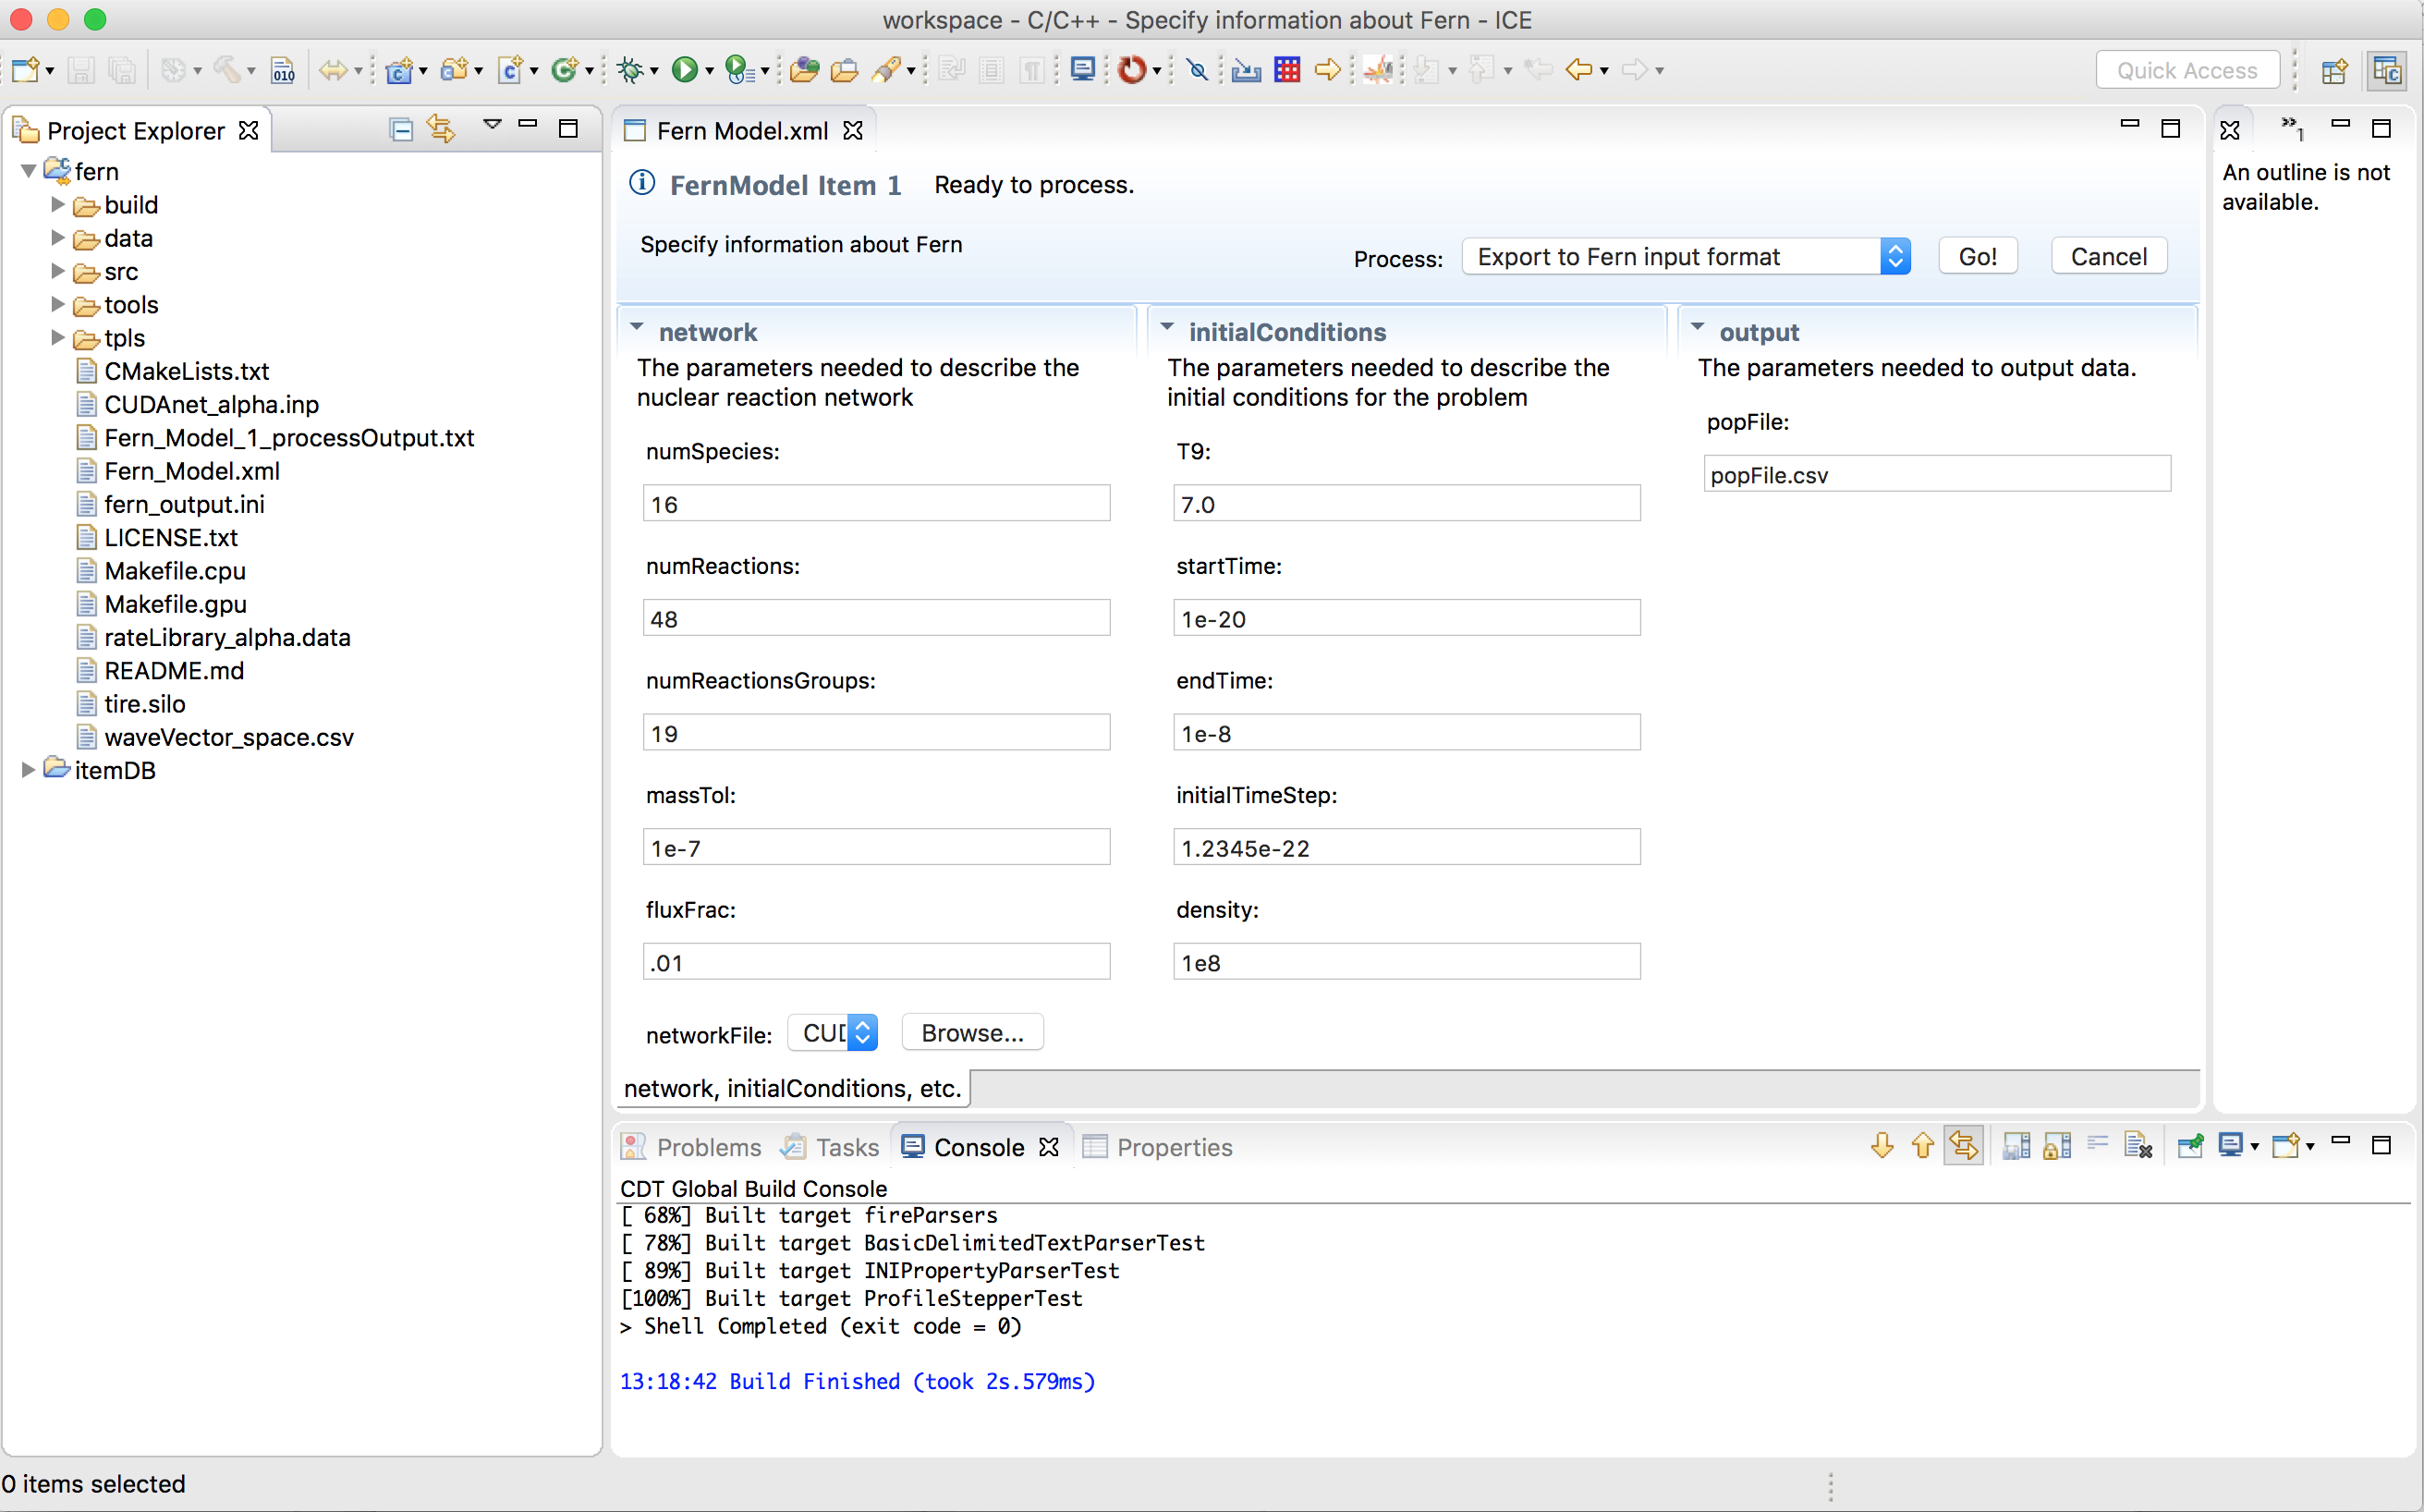
\includegraphics[width=\textwidth]{figures/fernmodelItem}
\end{center}
Here you can modify the various defaults with the values you would like for a
given Fern simulation. Once done, simply save the Item and click the
\texttt{Go!} button. This will execute the process of creating a new INI Fern
input file for use with the Fern Launcher. You can check the result by opening
the \texttt{fern\_config.ini} file, as shown below.
\begin{center} 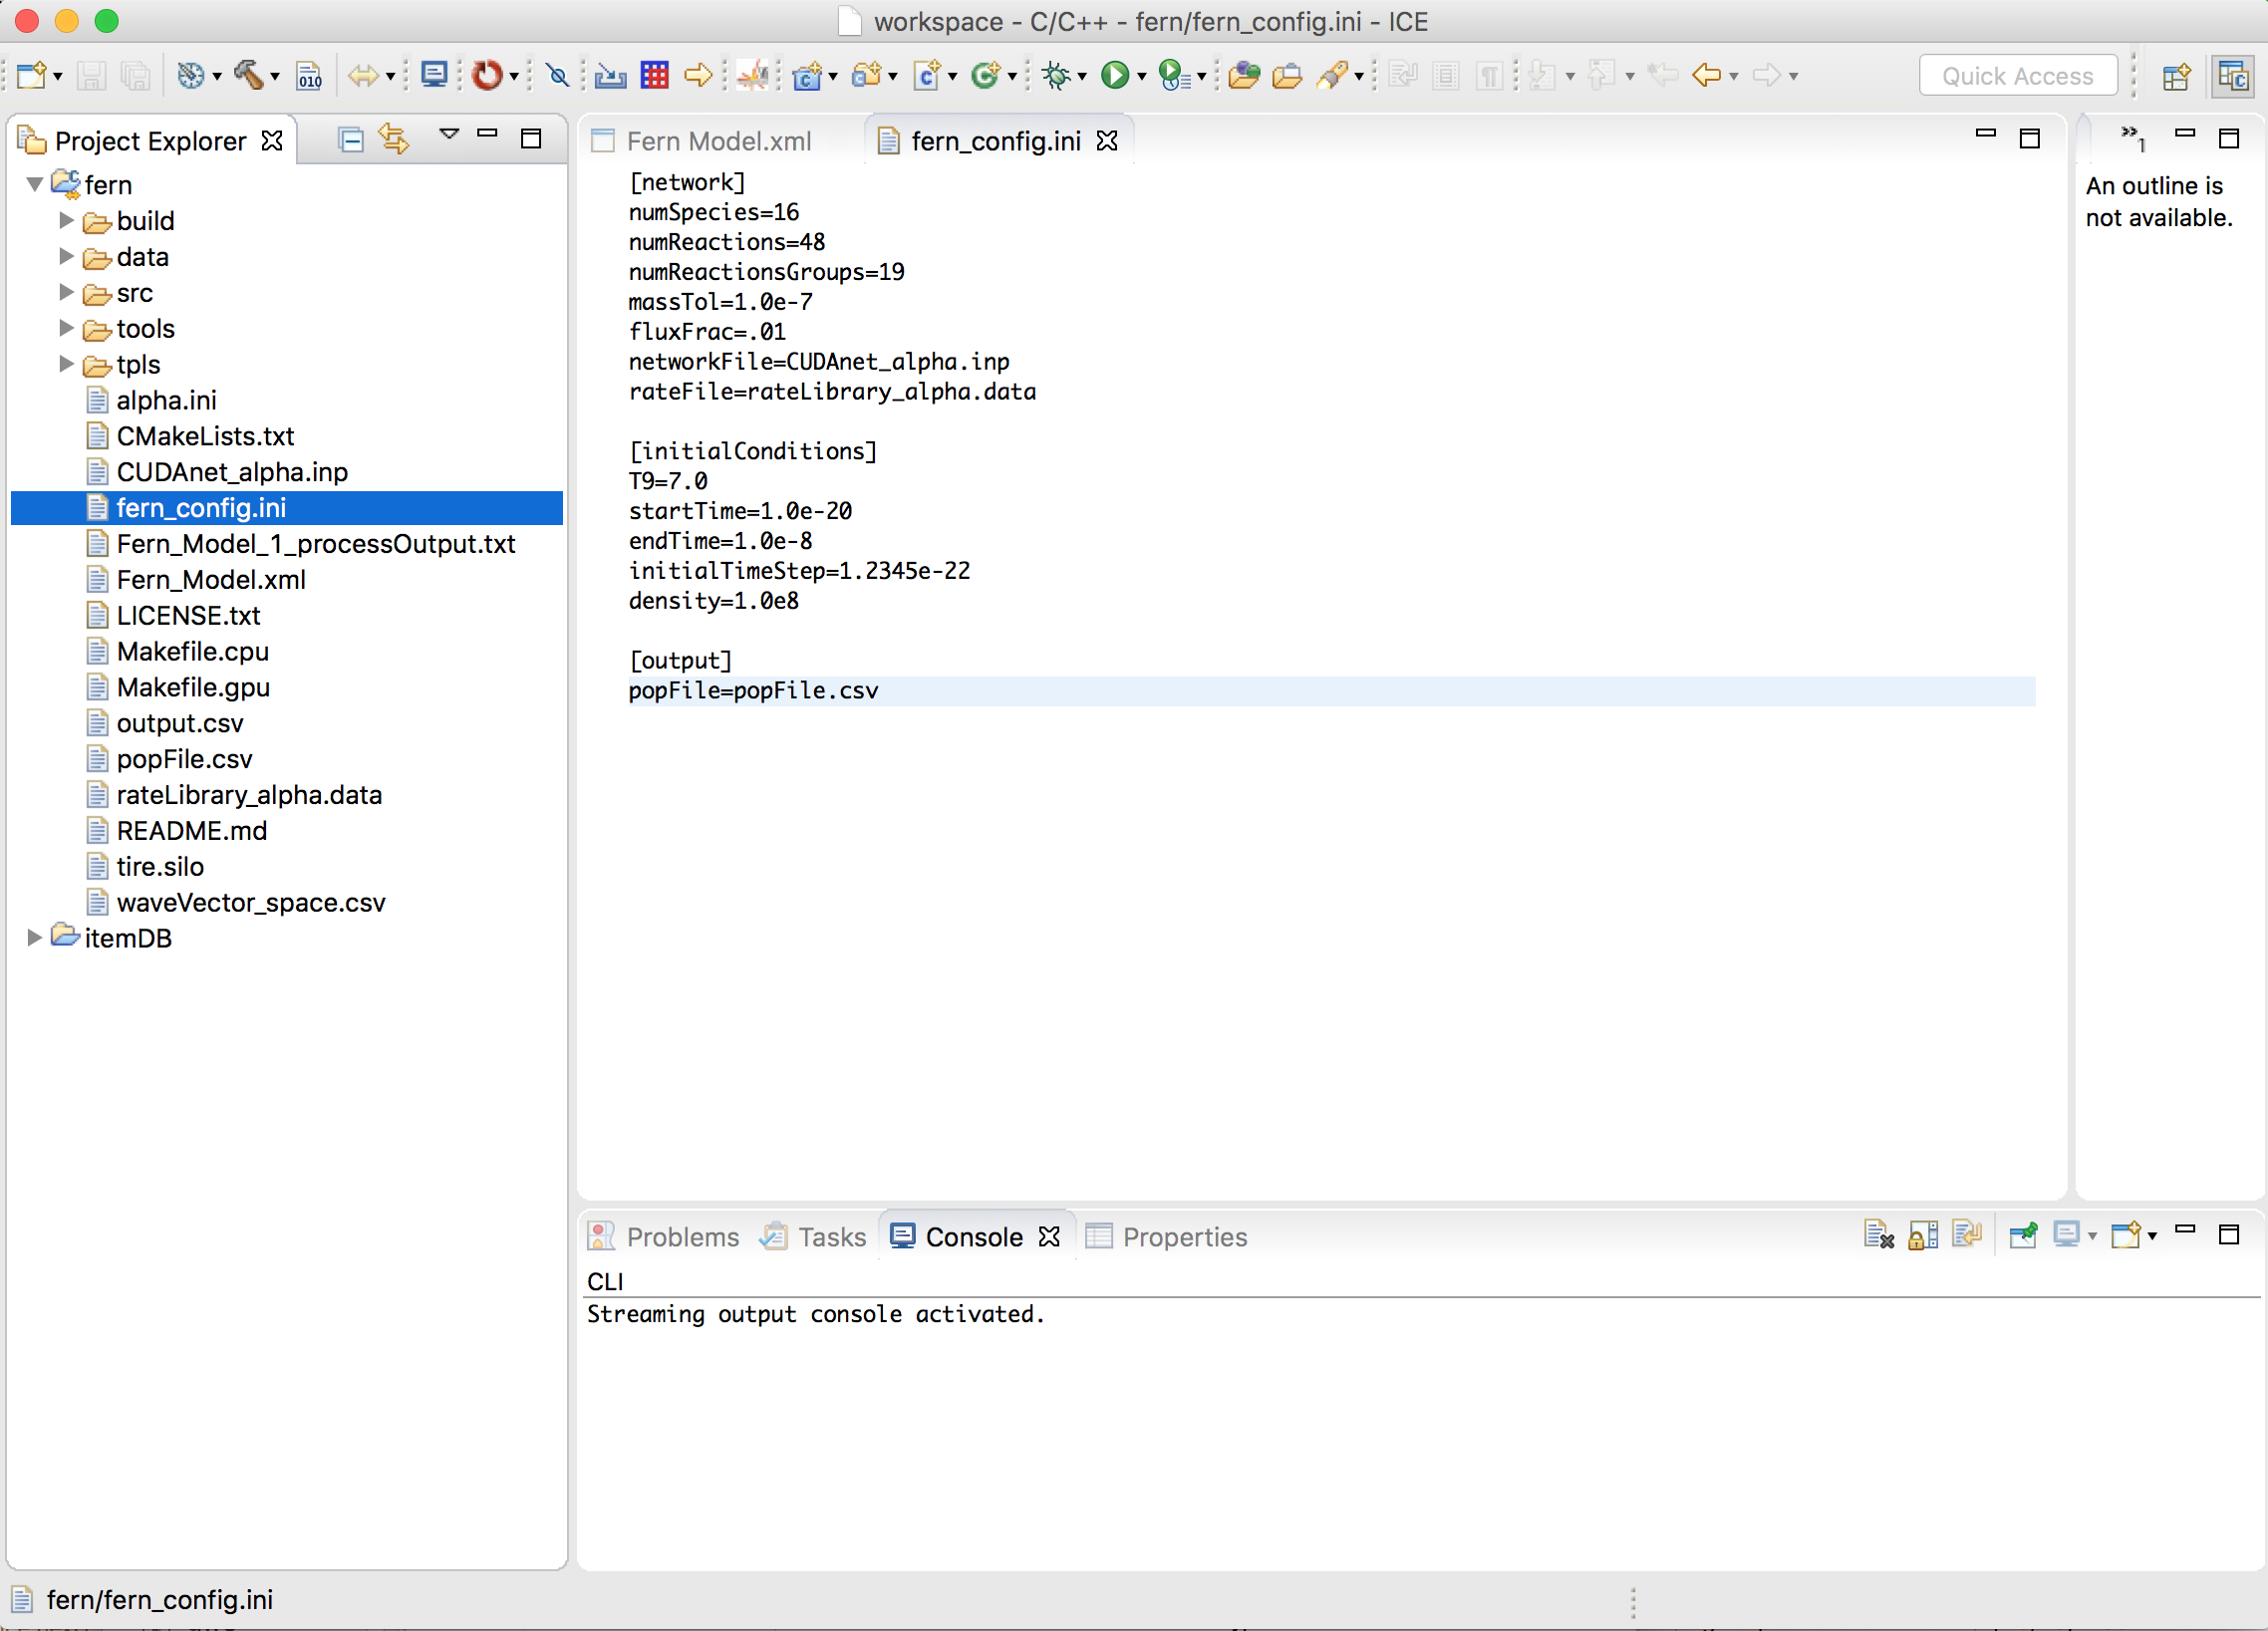
\includegraphics[width=\textwidth]{figures/result}
\end{center}

\subsection{Creating a Local Launcher}

Now you can similarly create a new FERN launcher. Note that as FERN is not
installed locally, we will not acutally launch the program using this method.

After creating the Launcher,
you should see a view like below. 
\begin{center} 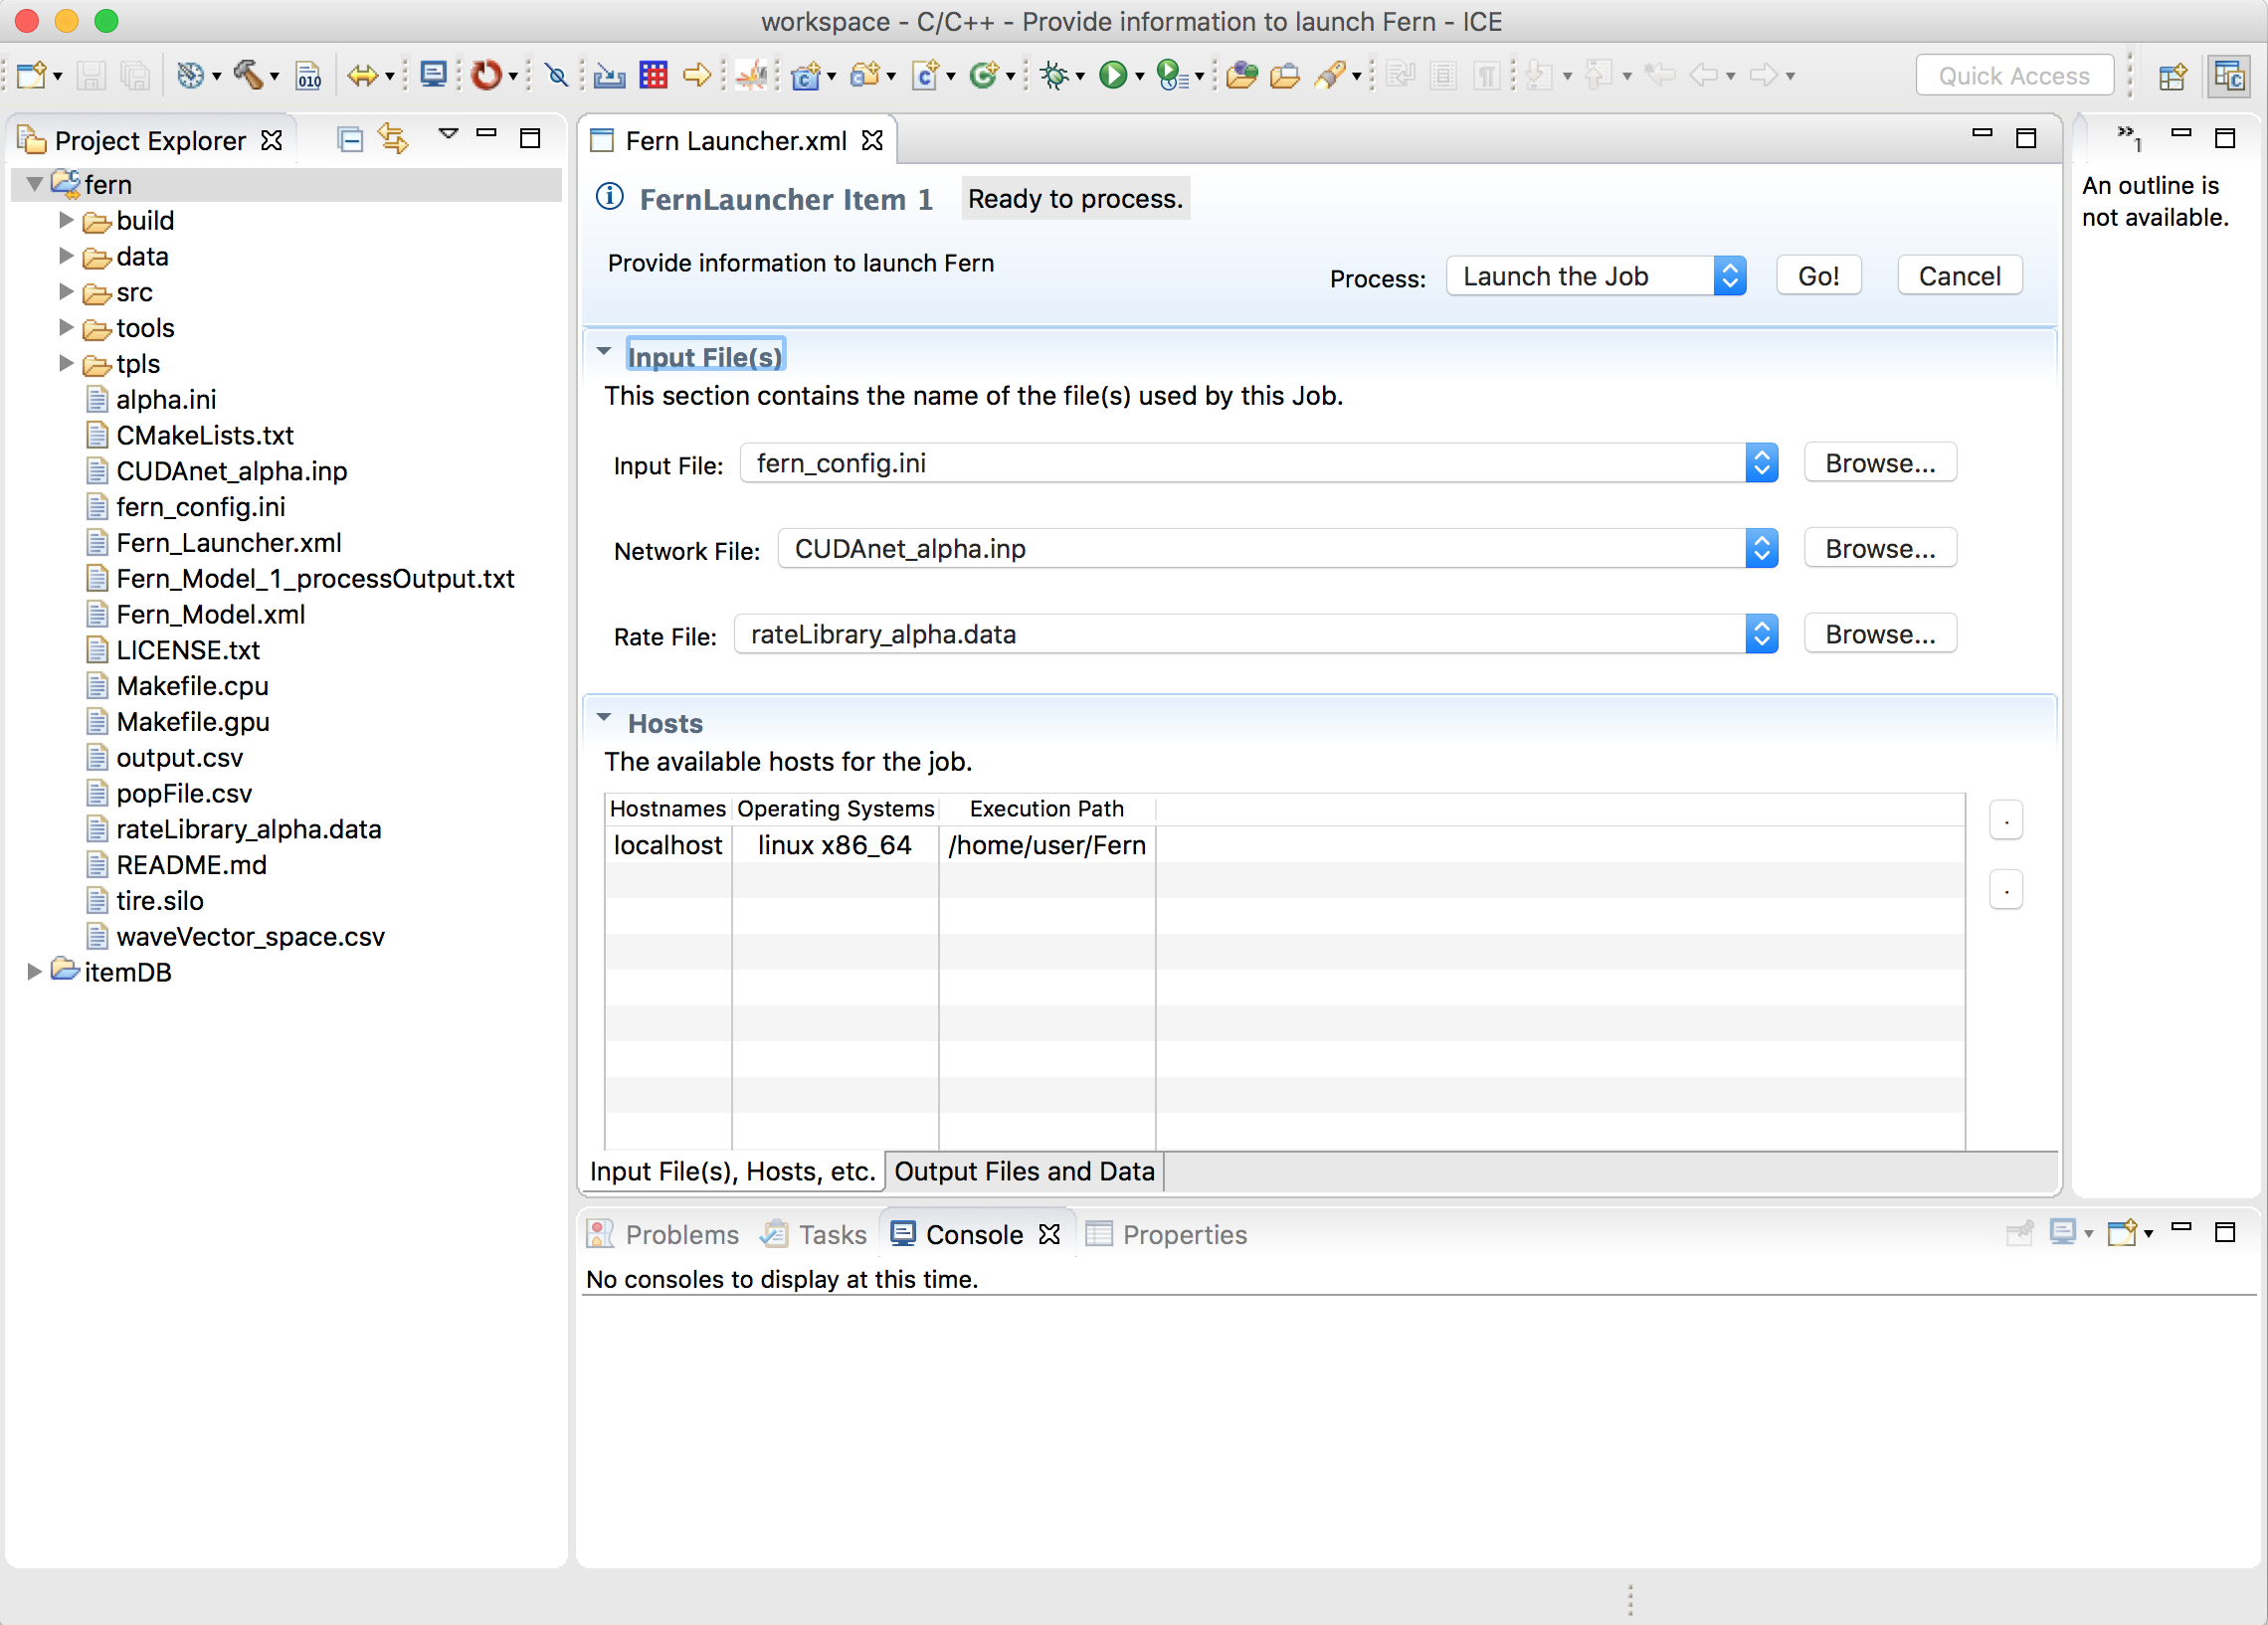
\includegraphics[width=\textwidth]{figures/launcher}
\end{center}
To configure a launch, simply set the correct
input file, along with its dependent network and rate files. 

At this point, if you had FERN built on your local machine, or if you had it
built on some remote host, you could configure that in the Hosts table. ICE
would then execute FERN based on that input. 

After the execution you should see the results in the Console, as shown below.
\begin{center} 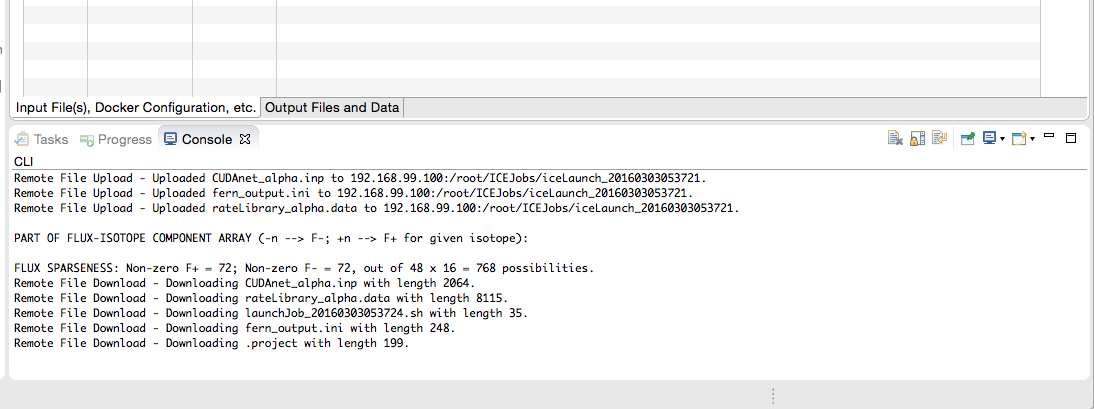
\includegraphics[width=\textwidth]{figures/launcherResult}
\end{center}
The execution should have produced a CSV file with the computed populations. You
can double-click that file to view them graphically in the ICE Plot Editor. 

\subsection{Creating a Remote Launcher}

Launching FERN remotely involves creating a \textit{Parallel launch
configuration}.
This procedure is not yet integrated with the ICE launcher, but will be
available in the next release of ICE.

A Parallel launch configuration for your application is created as follows:

\begin{enumerate}
  \item Select the \texttt{Run $\rightarrow$ Run Configurations\ldots} menu
  \item Click on the \texttt{Parallel Application} entry, then click the
  \texttt{New} button
  \item From the \texttt{Target System Configuration} dropdown, select
  \texttt{Generic Torque Batch}
  \item From the \texttt{Please select a connection}, choose the \texttt{gordon}
  connection you created earlier
  \item Click \texttt{Yes} when asked if you would like to run a command on the
  remote system (optionally check the box to not ask again)
  \item After a few seconds, you should see the job submission form
  \item Select \texttt{normal} for the queue
  
  \begin{center} 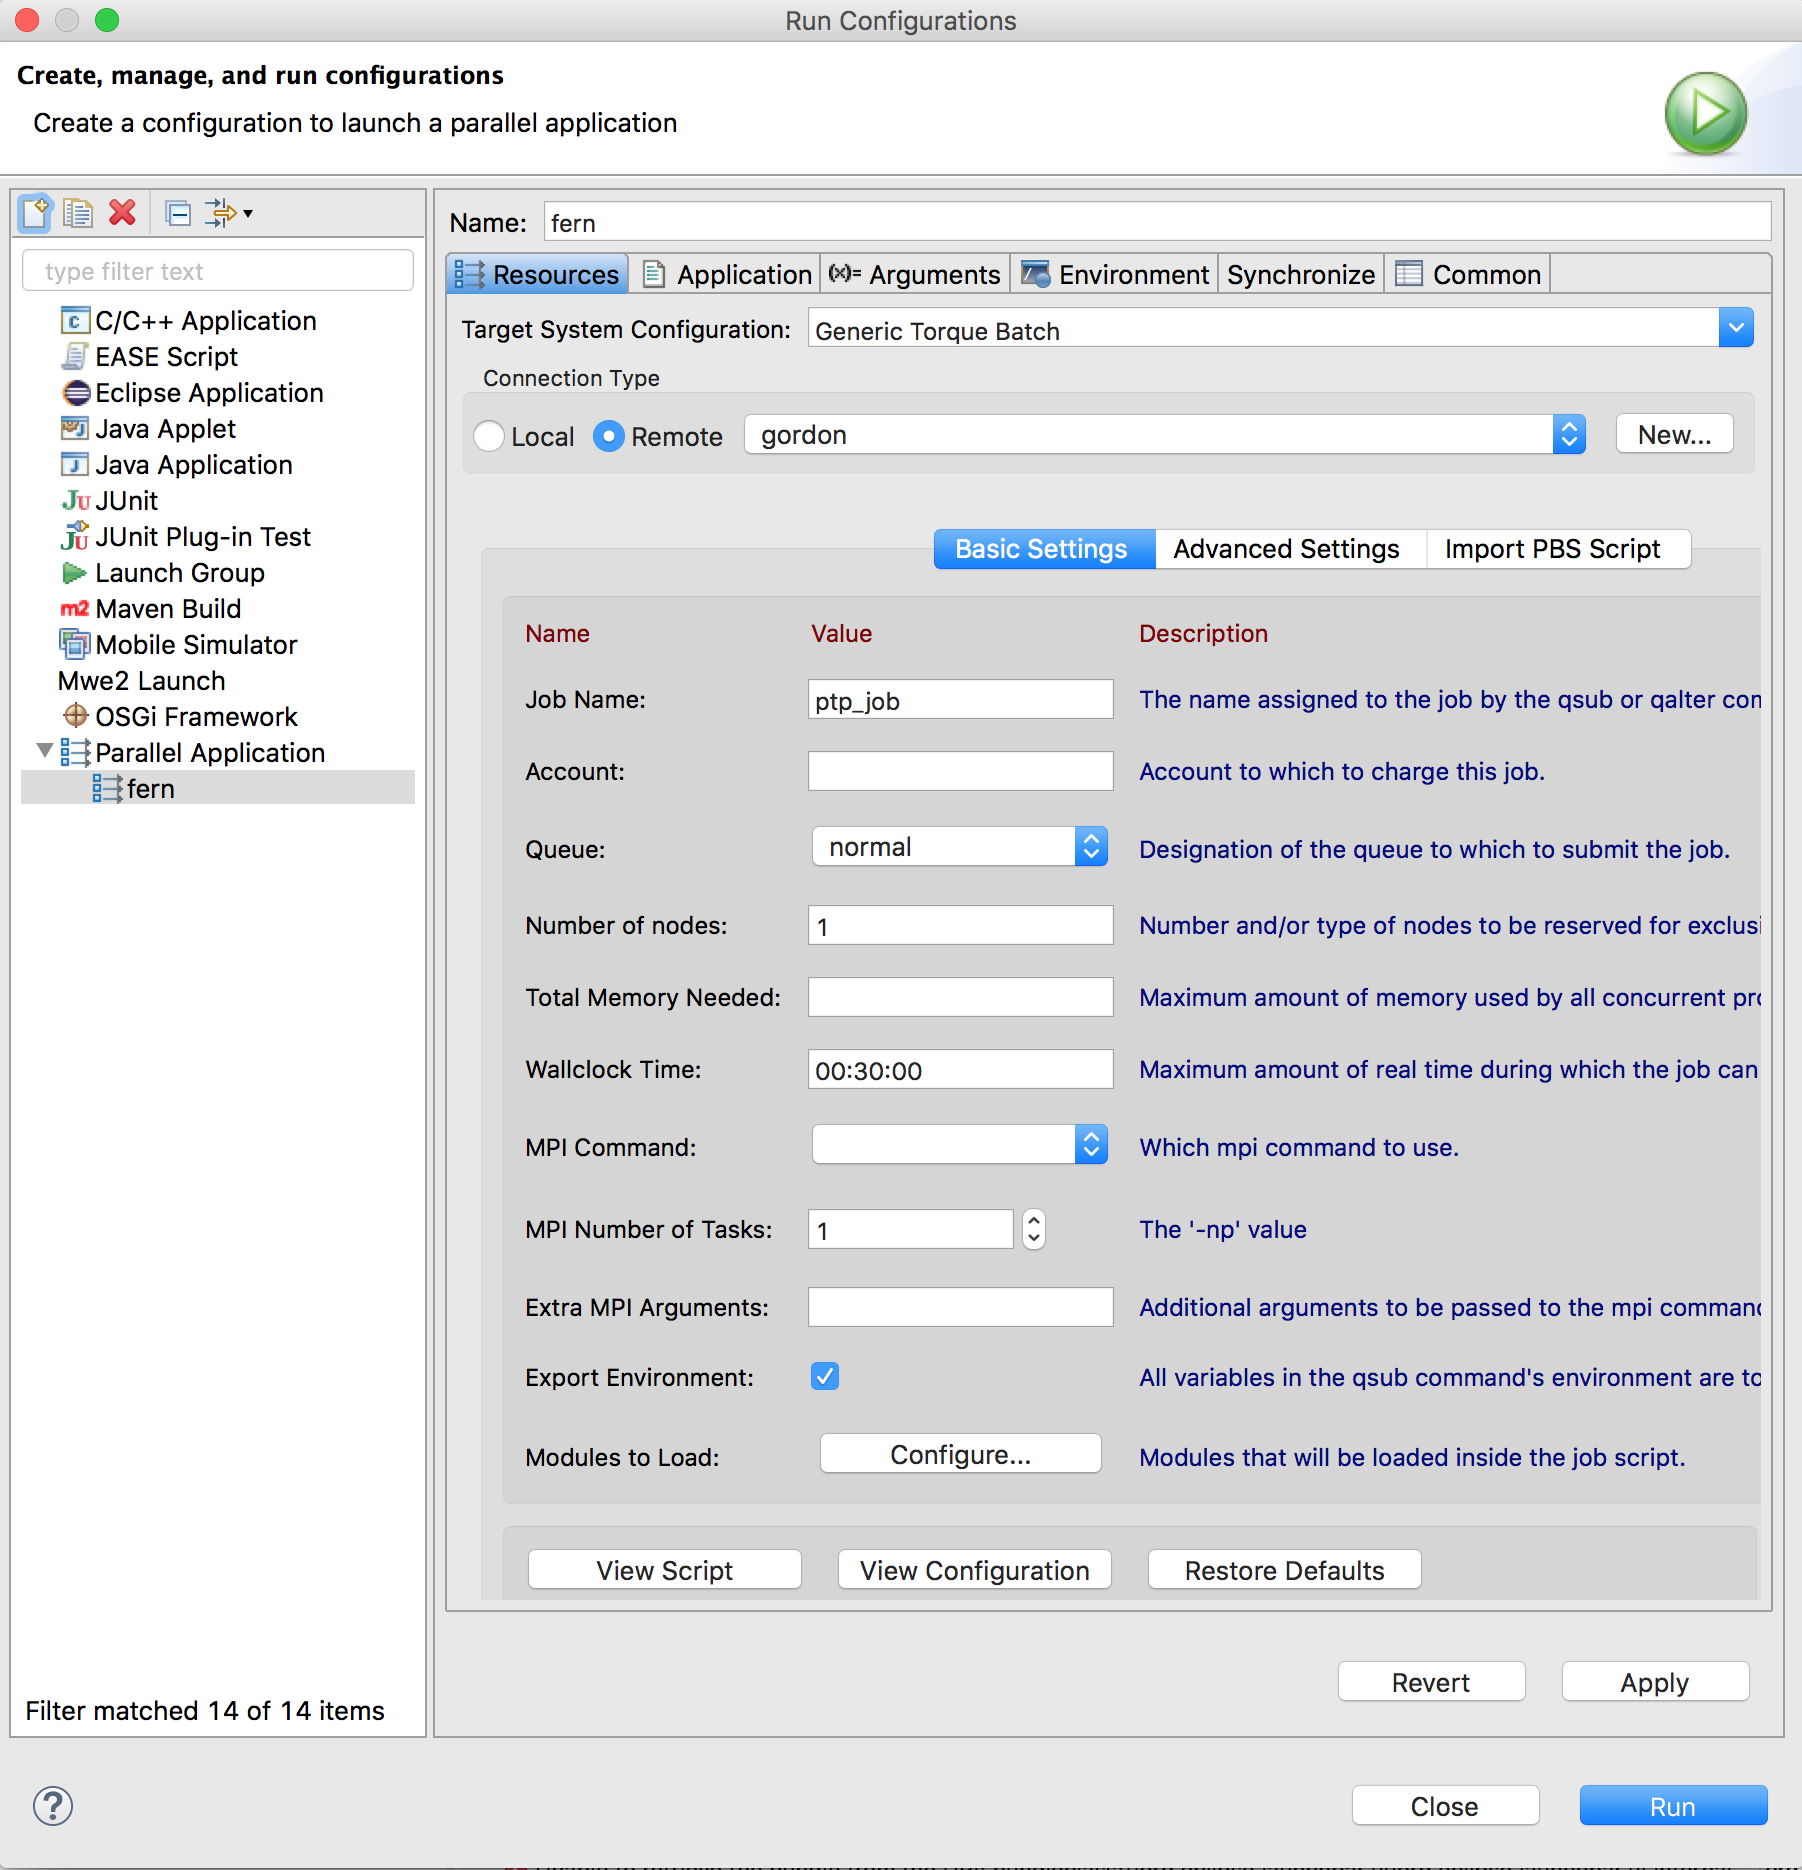
\includegraphics[width=\textwidth]{figures/runConfiguration}
  \end{center}
  
  \item Switch to the \texttt{Application} tab
  \item If the project field doesn't contain anything, click \texttt{Browse} and
  choose the \texttt{fern} project
  \item Click \texttt{Browse} next to the \texttt{Application program} field,
  open the \texttt{build} directory, select \texttt{fern-exec}, then click
  \texttt{OK}
  
  \begin{center} 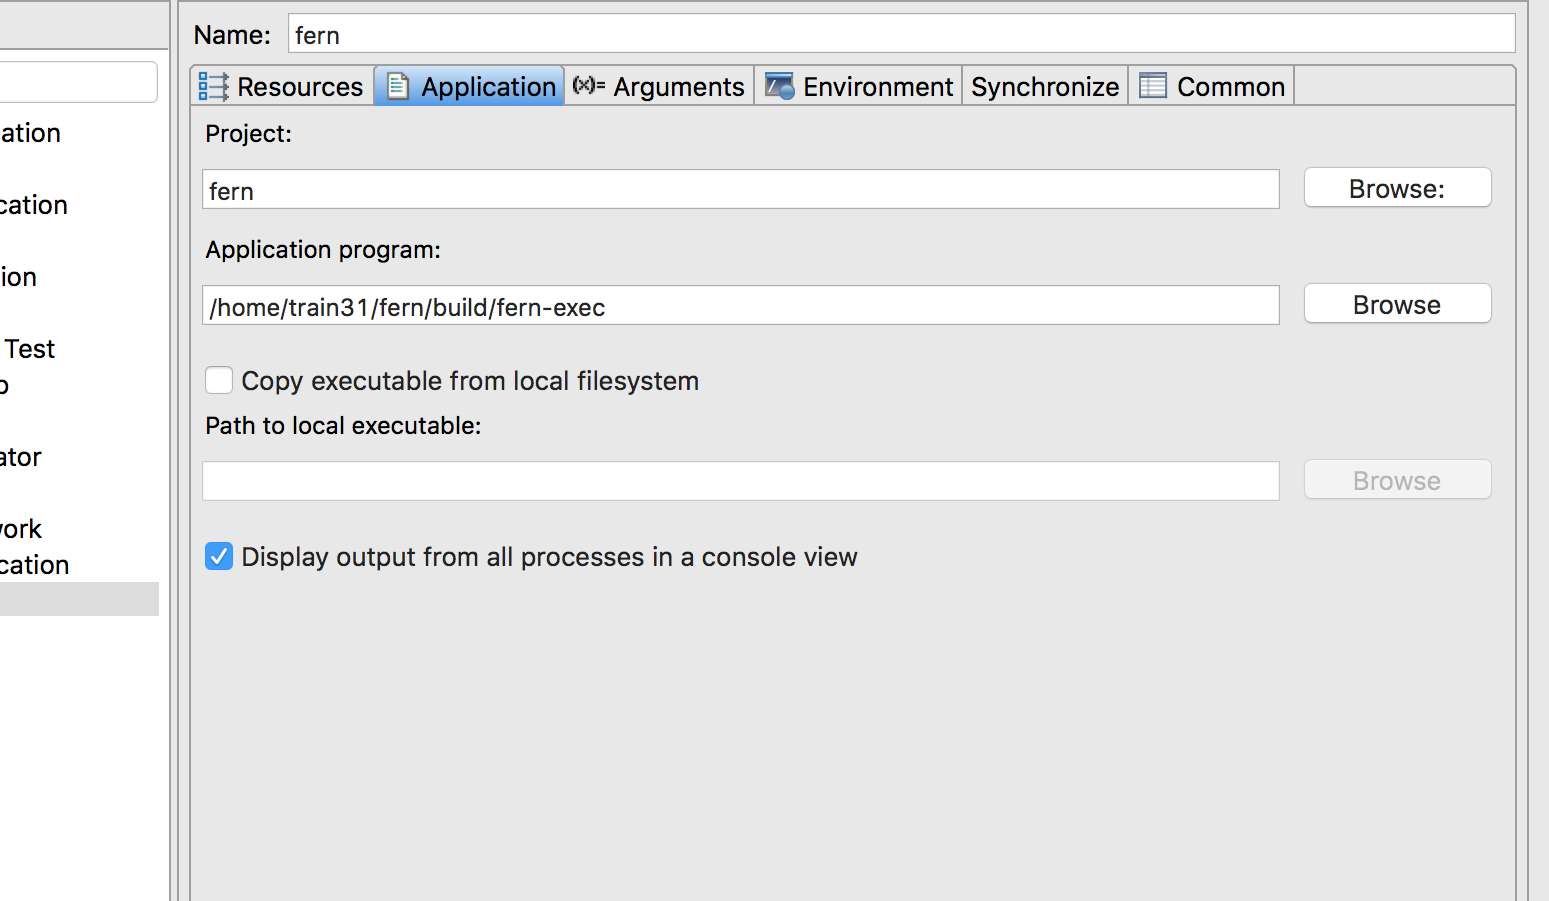
\includegraphics[width=300]{figures/applicationTab}
  \end{center}
  
  \item Switch to the \texttt{Arguments} tab and enter the name of the
  outputfile you chose in the \texttt{FernModel} file
  \item Uncheck \texttt{Use default working directory}, click on the
  \texttt{Browse} button, select the \texttt{fern} directory in the browser and
  click \texttt{OK}
  
  \begin{center} 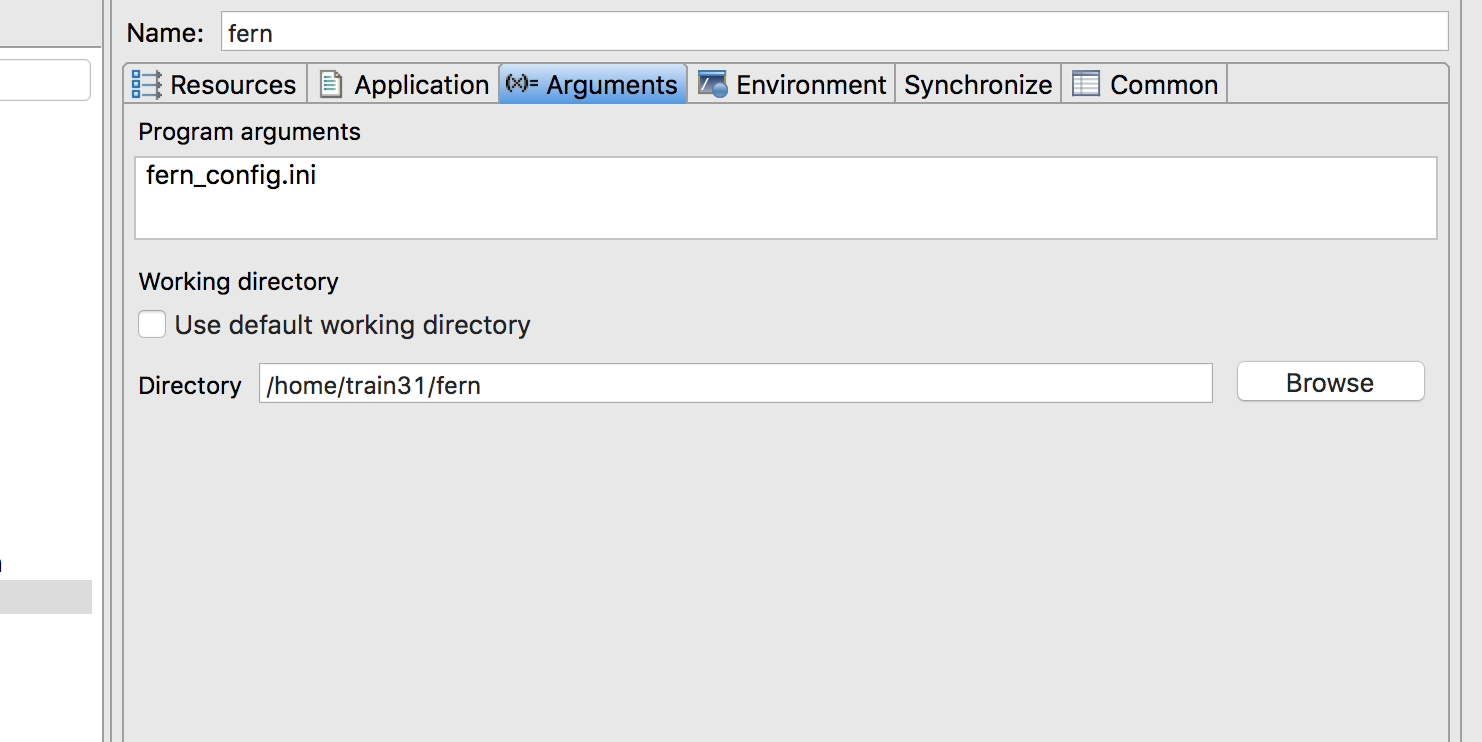
\includegraphics[width=300]{figures/argumentsTab}
  \end{center}
  
  \item Click \texttt{Run} to submit the job 
\end{enumerate}

During the job submission, you will be asked if you would like to switch to the
\texttt{System Monitoring} perspecive. Click \texttt{Yes} to see this feature.
The image below shows a typical instance of this perspective in action.

\begin{center} 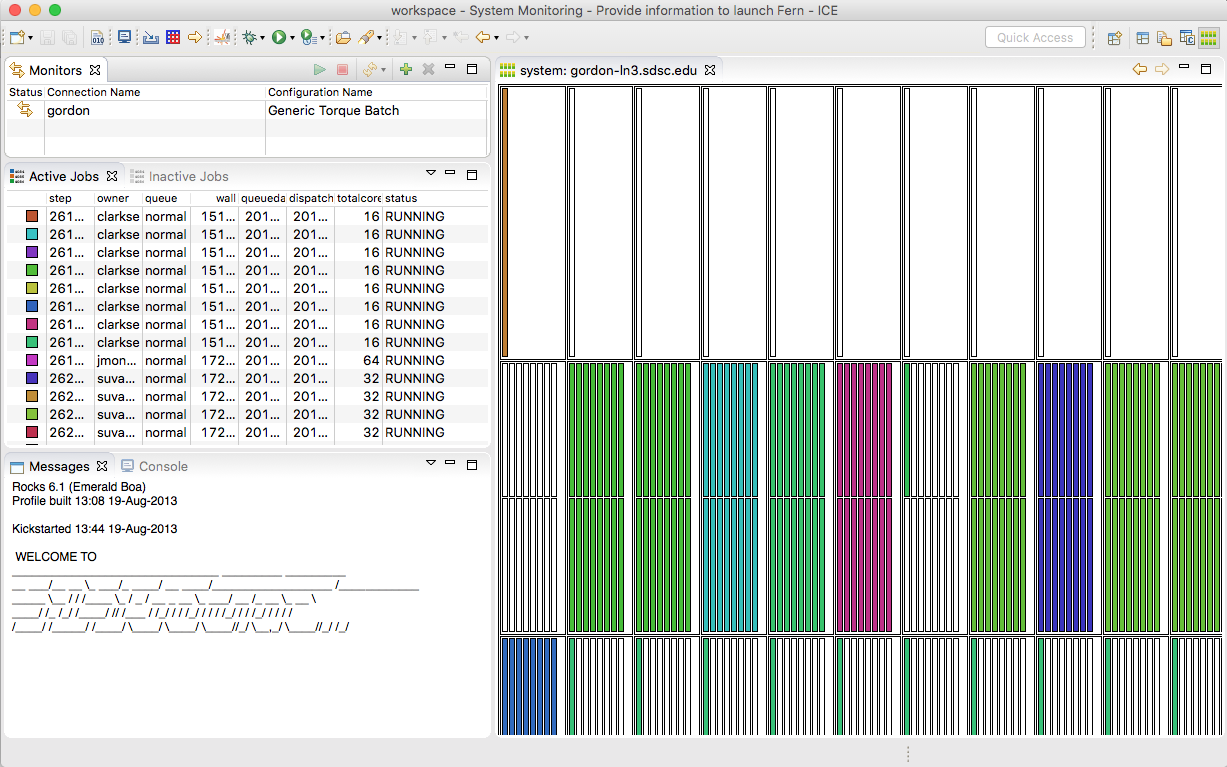
\includegraphics[width=\textwidth]{figures/sysMon}
\end{center}

Click on the \texttt{Inactive Jobs} view and scroll to the bottom. You should
see a job from your username that is either submitted or completed. When the job
is completed, you can switch back to the \texttt{C/C++ Perspective}.

\begin{center} 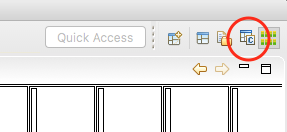
\includegraphics[width=200]{figures/cppPersp}
\end{center}

In the \texttt{Project Explorer} view, click on the \textit{synchronize}
button to copy the output files back to your local machine. 

\begin{center} 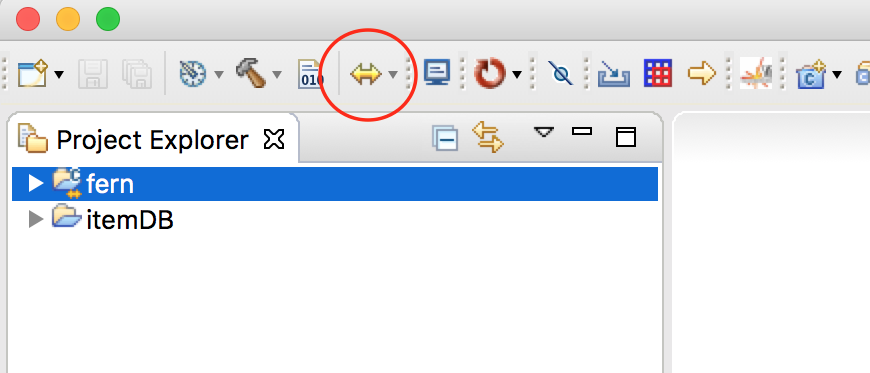
\includegraphics[width=200]{figures/syncButton}
\end{center}

If the project is not already open, you can open it now and
you should see the resulting CSV file. Double click on this file to launch the CSV viewer.



\chapter{Adding Visualization to your Application}
\graphicspath{{../../resourceComponents/src/}}
Resource Components are ICE Components which contain a grid of visualization
resources. These resources can display files from a variety of sources,
such as CSV files or VisIt visualizations. Geometry and Mesh editors allow for
editing of shapes or meshes. All three can be added to an Item to offer
visualization of data.

\section{Prerequisites}

You will need access to an installation of VisIt version $2.9.2$. There is a copy of the
software in the VisIt folder of your USB drive. Windows users should open the Windows installer, while users of
other OSs can just copy the appropriate folder onto their machine.

\section{Adding the Components}

We will be adding the visualization components to the model made in the
previous section, so return to your original ICE window, closing the launched
instance. For convenience, you can copy and paste the code from the
XSEDEVisualizationeModel.java in the org.eclipse.ice.demo.visualization.model
package. Its location can be seen in figure \ref{fig:demostructure}.

\begin{figure}[!h]
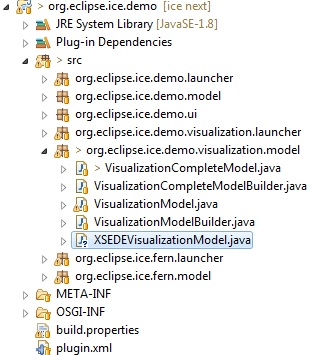
\includegraphics[width=200]{images/XSEDEDemoPackageStructure}
\centering
\caption{The package structure for org.eclipe.ice.demo bundle}
\label{fig:demostructure}
\end{figure}

First, copy and paste the following example code into the end of your Item's
setupForm() method. You can also find this code in
XSEDEVisualizationModel's setupForm() method, but be sure to note the
comments specifying where to begin and end copying. 

{\small
\begin{verbatim}
		//Create the resource component
		ResourceComponent resourceComponent = new ResourceComponent();

		//Set the component's data members
		resourceComponent.setName("Resource Component");
		resourceComponent.setDescription("Results");
		resourceComponent.setId(1);

		//Declare the files and resources
		VizResource csvResource = null;
		VizResource visItResource = null;
		IFile csvFile = null;
		IFile visItFile = null;


		//If the file was found, create the CSV resource and add it to the component
		try{
			
			//Open the files
			csvFile = ResourcesPlugin.getWorkspace().getRoot().getProject("itemDB").getFile("fib8.csv");
			visItFile = ResourcesPlugin.getWorkspace().getRoot().getProject("itemDB").getFile("tire.silo");
			
			//If the file was found, create the CSV resource and add it to the component.
			if(csvFile.exists()){
				csvResource = new 
		                    VizResource(csvFile.getLocation()
		                    .toFile());
		    	resourceComponent.addResource(csvResource);
			}
				        
			//If the file was found, create the VisIt resource and add it to 
			//the component
			if(visItFile.exists()){
				visItResource = new 
		                    VizResource(visItFile.getLocation()
		                    .toFile());
				resourceComponent.addResource(visItResource);
			}
		}
		catch(IOException e){
			e.printStackTrace();
		}

		//Create the geometry component
		ShapeController geometryRoot = new ShapeController(new
		    Shape(), new BasicView());
		GeometryComponent geometryComponent = new 
		    GeometryComponent();
		geometryComponent.setGeometry(geometryRoot);
		geometryComponent.setName("Geometry Editor");

		//Create mesh component
		MeshComponent meshComponent = new MeshComponent();
		meshComponent.setName("Mesh Editor");

		//Add the components to the form
		form.addComponent(resourceComponent);
		form.addComponent(geometryComponent);
		form.addComponent(meshComponent);	
		
		// Set the context on the Form
		form.setContext("visualization");
\end{verbatim} 
}

This will cause errors in your file. To resolve them, first open the MANIFEST.MF
file in your project's META-INF folder, switch to the \texttt{Dependencies} tab,
and click the \texttt{Add} button under the \texttt{Imported Packages} section,
both highlightted in figure \ref{fig:manifest}. Select
\texttt{org.eclipse.eavp.viz.datastructures}, press \texttt{OK}, and save the
file. You can then return to your model file, hover over the underlined code
for each of the errors until a menu pops up, and select the option to add a
package to the imported packages, as seen in figure \ref{fig:hover}. Repeat the process, this time choosing the option to import the class. Save the file when the hover menu no longer appears over
errors.

\begin{figure}[!h]
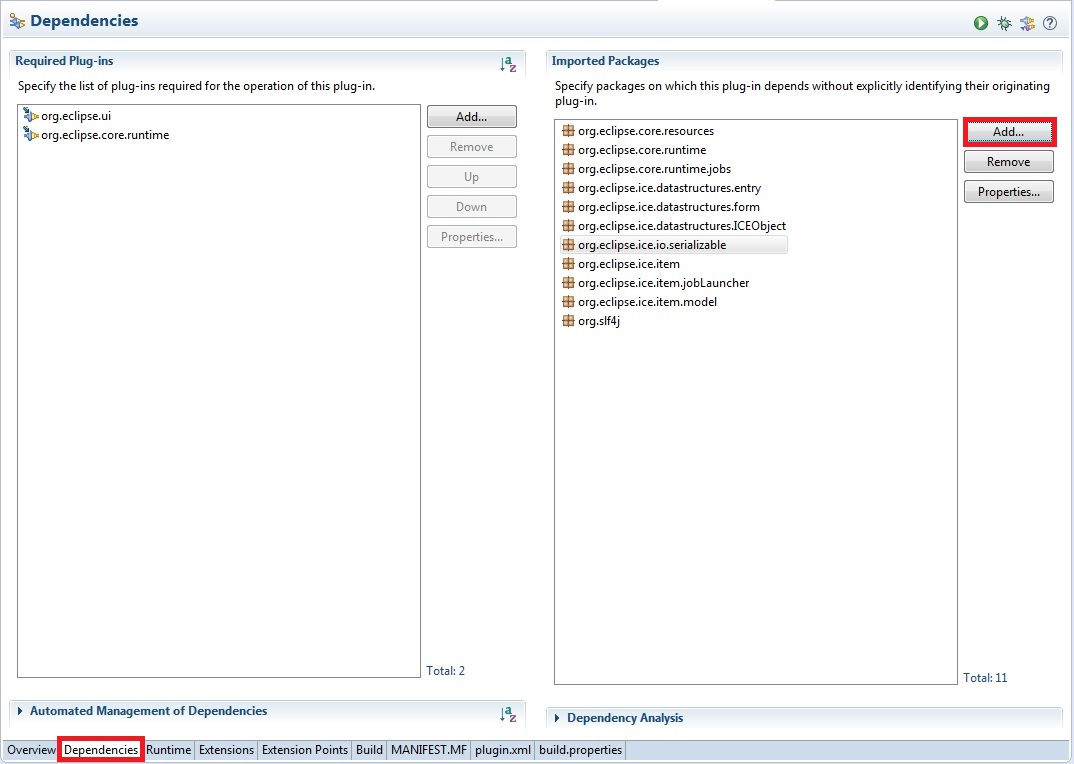
\includegraphics[width=\textwidth]{images/ManifestDependencies}
\centering
\caption{The Manifest dependencies view}
\label{fig:manifest}
\end{figure}

\begin{figure}[!h]
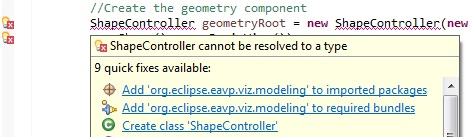
\includegraphics[width=\textwidth]{images/ErrorHoverMenu}
\centering
\caption{The menu displayed when hovering the mouse over code with an error.}
\label{fig:hover}
\end{figure}

This code will add a Resource Component, Geometry Component, and Mesh Component
to your Item and load tire.silo into the Resource Component. When done, launch
ICE again, using \texttt{Developer} $rightarrow$ \texttt{ICE} $rightarrow$
\texttt{Launch New Instance}.

\section{Using the Resource Component}

ICE uses an instance of VisIt, a visualization code from Lawrence Livermore
National Laboratory, running in another process for visualization. ICE can also
use ParaView, but this tutorial will only cover VisIt, as the processes for
conencting to ParaView and using a ParaView Plot Editor are largely similiar to
those for VisIt.

\subsection{Establishing a VisIt Connection}

In order to visualize resources containing VisIt files, ICE must be connected to
a running VisIt installation. To set up this connection, select \texttt{Windows}
$\rightarrow$ \texttt{Preferences...} in ICE's menu bar. (On Mac OS X,
\texttt{Preferences} is instead located under \texttt{ICE} in the menu
bar.)

\begin{figure}[!h]
\includegraphics[width=12cm]{images/ICEPreferences}
\centering
\caption{The ICE \texttt{Preferences Menu} for Windows and Linux. It will be
located under \texttt{ICE} instead of \texttt{Window} on Mac.}
\label{fig:icepreferences}
\end{figure}


Select \texttt{Visualization} $\rightarrow$ \texttt{VisIt} in the tree on the
left side of the \texttt{Preferences} window.

\begin{figure}[!h]
\includegraphics[width=12cm]{images/VisualizationPreferences}
\centering
\caption{The \texttt{VisIt} preferences page in the \texttt{Preferences}
dialog. The hilighted button will add a row for a new connection to the table.}
\label{fig:visualizationpreferences}
\end{figure}


Press the button with a "+" symbol in the upper right of the
\texttt{Preferences Menu} (highlighted in Figure
\ref{fig:visualizationpreferences}) to add a new row to the table.
Click on the \texttt{Path} cell of the new row and put the path of your installation of VisIt.

For example, on \texttt{Windows}, if assuming a username of "username", and
VisIt was installed in the default location, the path will be:

\texttt{C:\textbackslash Users\textbackslash
username\textbackslash AppData\textbackslash Local\textbackslash
Programs\textbackslash LLNL\textbackslash VisIt 2.9.2.}

On \texttt{Linux}, the path will be based on where you extracted the 
visit2\_9\_2.linux-x86 folder, ending with /visit2\_9\_2.linux-x86\_64. If
you unzipped it to the desktop, it will be:
 
\texttt{/home/username/Desktop/visit2\_9\_2.linux-x86\_64}

On \texttt{Mac OS}, the path will be based on the location you put the Visit
application. If placed in the Applications folder it will be

\texttt{/Applications}

Press \texttt{Apply}, then \texttt{OK}, both in the lower right hand corner of
the \texttt{Preferences Menu}.
ICE will now open and connect to this VisIt installation each time ICE is opened.

\subsection{Opening Your Item}
Before opening your new Item, select the itemDB folder in the \texttt{Project
Explorer} and press the import button, highlighted below.

\begin{figure}[!h]
\includegraphics[width=12cm]{images/ImportButton}
\centering
\caption{ICE's \texttt{import} button.}
\label{fig:importbutton}
\end{figure}

Select the files you want to visualize and click OK. For the tutorial,
this should be the tire.silo file from the Fern synchronized project directory.
You should now see the file within the itemDB folder.

Select \texttt{File} $\rightarrow$ \texttt{New} $\rightarrow$
\texttt{Other\ldots} from the toolbar.
In the new dialog, select the \texttt{Create Item Wizard} and hit \texttt{Next}.
Then select \texttt{Visualization Model} and press \texttt{Finish}. You can also select the
\texttt{Visualization Model (Pre-completed)} if you skipped the first part of
the tutorial.

Finally, switch to the ICE Perspective to ensure that the necessary Views will
be open. To do this, click the \texttt{Open Perspective} button in the upper right
of the workbench screen.

\begin{figure}[!h]
\includegraphics{images/ICE_OpenPerspective}
\centering
\caption{ICE's \texttt{Open Perspective} button.}
\label{fig:openpersepctive}
\end{figure}

In the dialog, select \texttt{ICE} and press {OK}.

\subsection{Managing the Resources}

Your Item should look like this when it loads.

\begin{figure}[!h]
\includegraphics[width=12cm]{images/ItemTabs}
\centering
\caption{The \texttt{Visualization Model} after it is initially opened.
Hilighted in the lower left are the tabs for the three components, the
\texttt{Geometry Editor}, the \texttt{Mesh Editor}, and the \texttt{Resource
Component}.}
\label{fig:itemtabs}
\end{figure}

In the lower left of the \texttt{Visualization Model} are three tabs, hilighted
in Figure \ref{fig:itemtabs}.
Switch to the \texttt{Resource Component} tab in your Item and to the
\texttt{Resources} tab on the left, as shown below.

\begin{figure}[!h]
\includegraphics[width=12cm]{images/ResourcesTab}
\centering
\caption{The \texttt{ICE Perspective}'s \texttt{Resources} tab.}
\label{fig:resourcestab}
\end{figure}

Double click on the file named tire.silo to load it into the Resource
Component.

At the top left of the \texttt{Visualization Model} will be controls for the
component's layout.

\begin{figure}[!h]
\includegraphics{images/ResourceComponentControls}
\centering
\caption{The layout controls for the \texttt{Resource Component}.}
\label{fig:resourcecomponentcontrols}
\end{figure}

The \texttt{Clear} button will close all plots in the component. The other two
controls will allow you to specify the number of rows and columns in the grid.
Be careful when reducing them, as any plots which no longer fit in the grid will
be closed.

If you hover over a plot, a button will appear in its upper left hand corner.
Clicking it will close that plot. 

\begin{figure}[!h]
\includegraphics[width=12cm]{images/ClosePlotButton}
\centering
\caption{The X button in the upper left will close the plot.}
\label{fig:closeplotbutton}
\end{figure}

\subsection{Interacting with VisIt Plots}

\begin{figure}[!h]
\includegraphics[width=12cm]{images/VisItPlot}
\centering
\caption{An example of a file open in VisIt displayed in a \texttt{Plot
Editor}.}
\label{fig:visitplot}
\end{figure}

A VisIt plot will contain a 3D visualization of some model. You can click and
drag within the plot to rotate the image and zoom by scrolling your mouse wheel.
Right clicking in the plot will open a context menu, providing options for how
the model will be displayed.

At the bottom of the plot will be a series of controls for animation. If your
plot does not have time series data, they will be greyed out. 

\begin{figure}[!h]
\includegraphics[width=8cm]{images/TimeSliderWidget} 
\centering
\caption{The \texttt{Plot Editor}'s animation controls.}
\label{fig:timesliderwidget}
\end{figure}

The plot can be set to display an arbitrary time step by either dragging the
slider or by typing a time into the box to its left.

\subsection{Editing 3D Structures}

ICE also contains capabilities to render graphics with the Geometry Editor and
Mesh Editor. Programatically populating these editors with custom input is
beyond the scope of this tutorial. However, what follows will be a brief
overview of the editors' functionality.

\subsubsection{The Geometry Editor}

Now switch to the \texttt{Geometry Editor} tab in you the \texttt{Visualization
Model} and the \texttt{Shapes} tab on the left.

Clicking the \texttt{Add Primitives} button will display a drop down of
primitive shapes which can be added to the scene.

\begin{figure}[!h]
\includegraphics[width=12cm]{images/AddPrimitiveShape}
\centering
\caption{The \texttt{Add Primitives} button displays a menu of shapes to add.}
\label{fig:addprimitiveshape}
\end{figure}

Complex shapes can similarly be added using the \texttt{Add Complex} button.

\begin{figure}[!h]
\includegraphics[width=12cm]{images/AddComplexShape}
\centering
\caption{The \texttt{Add Complex} button can add a Union of shapes.}
\label{fig:addcomplexshape}
\end{figure}

Primitive shapes can be added under complex shapes by selecting anything beneath
the desired parent complex shape before adding the new primitive.

\begin{figure}[!h]
\includegraphics[width=12cm]{images/ComplexShapeTree}
\centering
\caption{An example of a constructive solid geometry tree in the
\texttt{Shapes} tab. Adding shapes with the highlighted leaf selected will
cause them to become children of Union 1.}
\label{fig:complexshapetree}
\end{figure}

The three other buttons are responsible for creating copies of or removing
selected shapes from the tree. 

The Transformation View, in the lower left of the workbench screen, has spaces
to set the rotation, scale, and translation of a selected object.

\begin{figure}[!h]
\includegraphics[width=12cm]{images/TransformationView}
\centering
\caption{The \texttt{Transformation View}.}
\label{fig:transformationview}
\end{figure}

\subsubsection{The Mesh Editor}

Now switch to the \texttt{Mesh Editor} tab in your Item and \texttt{Mesh
Elements} tab on your left.

Clicking within the grid will create a vertex, until the fourth completes the
polygon.

\begin{figure}[!h]
\includegraphics[width=12cm]{images/AddPolygon}
\centering
\caption{A new polygon, colored green because the user has not yet permanently
added it to the mesh.}
\label{fig:addpolygon}
\end{figure}

Click again to make the polygon permanent, signified by turning purple, or hit
\texttt{Esc} to cancel.

\begin{figure}[!h]
\includegraphics[width=12cm]{images/NewPolygon}
\centering
\caption{The polygon turns purple after clicking, showing that it has been
finished.}
\label{fig:newpolygon}
\end{figure}

The \texttt{Mode} button in the top left allows you to switch between
\texttt{Add Elements} mode, used previously, and \texttt{Edit Elements} mode.

\begin{figure}[!h]
\includegraphics[width=8cm]{images/EditMode}
\centering
\caption{The \texttt{Mode} button allows switching between \texttt{Edit
Elements} mode and \texttt{Add Elements} mode.}
\label{fig:editmode}
\end{figure}

In edit mode, you can click a vertex (or vertices) to select them. 

\begin{figure}[!h]
\includegraphics[width=12cm]{images/SelectedVertex}
\centering
\caption{A selected vertex will turn blue.}
\label{fig:selectedvertex}
\end{figure}

You can click and drag a vertex to move all selected vertices around the grid.

\section{Further Reading}

This tutorial has only given a brief overview of the ways in which you can use
ICE's visualization tools. For more detailed information, look under the
\texttt{docs} folder in the ICE repository. The visualization folder contains a
tutorial on the CSV and VisIt plots, while the geometryEditor and meshEditor
folders have tutorials on the geometry and mesh editors, respectively. 

\chapter{Exploring Visualization in ICE}
\graphicspath{{../../geometryEditor/src/}}
\section{Overview} 

This tutorial will teach you how to
create your own ICE Items via the built in tools within ICE.  To demonstrate
these tools, we will walk through the development of an ICE Item project for the
FERN code, a fast, efficient nuclear reaction network solver. 

After creating a new ICE Item plugin project, we will demonstrate how to
provide a few lines of code to get a Model Item showing in ICE that creates
input files for FERN. After that we will add a little code to the FERN
JobLauncher to be able to execute FERN locally, remotely, or via the
provided Docker image. Before we begin, ensure that you have ICE cloned
(Developer $>$ ICE $>$ Clone ICE or Developer $>$ ICE $>$ Import Local
Repository) into your workspace.


\section{Creating the Project}

\begin{figure}[h]
\centering
\includegraphics[width=\textwidth]{figures/comb12.png}
\label{fig:comb12}
\end{figure}

To create a new ICE Item project, navigate to \texttt{File $>$ New $>$ Other}
and open the \texttt{ICE Item Creation Wizards} folder and 
select \texttt{ICE Item Creation Wizard}. You will be met with a standard new
project wizard page, in which you can name your project.  We will call ours
\texttt{org.eclipse.ice.fern}. Once you have named your project click the \texttt{Next >} button.
\begin{center} \includegraphics[width=\textwidth]{figures/comb23} \end{center}
Now you are able to customize the plugin-specific portions of the project. 

On this page you need to tell the wizard what you want to use as a base
name for your item classes. We will call this one \texttt{Fern}. Then, we will
specify some information about how the item will handle input data.  Fern uses
the INI file format to specify data, so we will tell our item to use the built-in
functionality for INI files.  To do this select \texttt{INI} from the \texttt{File Format} dropdown.  

When you have entered all of the required information you can
click the \texttt{Finish} button to generate your new ICE Item plugin project.
When the project has finished generating you should be able to explore the code
that has been created.  Within the source directory there will be two packages,
each containing two Java classes:

\begin{itemize} 
    \item \texttt{org.eclipse.ice.fern.launcher} 
    \begin{itemize}
        \item \texttt{FernLauncher.java} 
        \item \texttt{FernLauncherBuilder.java}
    \end{itemize} 
    \item \texttt{org.eclipse.ice.fern.model} 
    \begin{itemize} 
        \item \texttt{FernModel.java} 
        \item \texttt{FernModelBuilder.java}
    \end{itemize} 
\end{itemize}

To add functionality to the project we need to edit
the \texttt{FernLauncher} and \texttt{FernModel} classes.

\section{Adding Functionality to the New Items}

\subsection{The Fern Model}

The \texttt{FernModel} will be responsible for creating and
validating input parameters for FERN, in the form of a new FERN input file.  In
order to make the generated code run there are several pieces of information that need to be changed.  First, we
will need to set up the basic Item idenfification information. This information
is set in the setupItemInfo() method. Modify the outputName to match the
following (or something of your choosing, with a .ini file extenstion).

\begin{lstlisting}[language=Java]
outputName = "fern_config.ini";
\end{lstlisting}

The String for the \emph{setName} method will serve as the display name
for this Item, so set it as \texttt{Fern Model}.
As for the String for \emph{setDescription}, this will also be used on the UI
for the Item, so provide some text like the following: \texttt{This Item constructs input files
for the FERN reaction network solver}. The export string will serve as the name
of the action that the user can select to write the provided data to file. Set
it to something like: \texttt{Export to INI}. You should now have a method that
looks like this:

\begin{lstlisting}[language=Java]
@Override
protected void setupItemInfo() {
	setName("Fern Model");
	setDescription("This Item constructs " +
	    "input files for the FERN reaction " +
	    "network solver"); 
	outputName = "fern_output.ini";   
	exportString = "Export to INI";
	allowedActions.add(0, exportString);
	ioFormat = "INI";
	defaultFileName = "";
}
\end{lstlisting}

The \emph{allowedActions.add()} line ensures that the export string is provided
to ICE as an allowed action, and displayed in the Item Process drop down.

With the identification information configured properly we can begin to
implement the Form for this Fern Model. This is done in the \emph{setupForm()}
method.
The generator has begun the process of implementing this method by instantiating
a Form for you to use, getting a reference to the IOService (which provides
IReader/IWriter realizations), and providing a commented out example of how to
fill out an ICE Form.

For this FERN input model, we want to add the following sections with data
entries: a network section with 
numSpecies, numReactions, numReactionGroups, massTol, fluxFrac, networkFile,
rateFile data entries, an initialConditions section with T9, startTime, endTime,
initialTimeStep, and density, and an output section with a single popFile
data entry.
To achieve this for this Item, we will need to add three
\texttt{DataComponents}, one for the network section, another for the
initialConditions section, and a final one for the outputs section. To each of
those DataComponents we will add appropriate IEntry instances for each of the data entries we have.

Add the following to your setupForm() method: 

\begin{lstlisting}[language=Java]

    // Create the network section
    DataComponent networkComp = new DataComponent();
    networkComp.setName("network");
    networkComp.setDescription("The parameters needed " +
        "to describe the nuclear " +
    	"reaction network"); 
    networkComp.setId(1);
    
    // Create the IEntries we need for this DataComponent
    StringEntry numSpecies = new StringEntry();
    numSpecies.setName("numSpecies");
    numSpecies.setDescription("The number of species to consider");
    numSpecies.setDefaultValue("16");
    
    StringEntry numReactions = new StringEntry();
    numReactions.setName("numReactions");
    numReactions.setDescription("The number of reactions to consider");
    numReactions.setDefaultValue("48");
    
    StringEntry numReactionGrps = new StringEntry();
    numReactionGrps.setName("numReactionsGroups");
    numReactionGrps.setDescription("The number of reaction " + 
    	"groups to consider"); 
    numReactionGrps.setDefaultValue("19");

    StringEntry massTol = new StringEntry();
    massTol.setName("massTol");
    massTol.setDescription("The mass tolerance to consider");
    massTol.setDefaultValue("1e-7");
    
    StringEntry fluxFrac = new StringEntry();
    fluxFrac.setName("fluxFrac");
    fluxFrac.setDescription("The flux fraction to consider");
    fluxFrac.setDefaultValue(".01");
    
    FileEntry networkFile = new FileEntry(".inp");
    networkFile.setProject(project);
    networkFile.setName("networkFile");
    networkFile.setDescription("The network file for this problem");
    
    FileEntry rateFile = new FileEntry(".data");
    rateFile.setProject(project);
    rateFile.setName("rateFile");
    rateFile.setDescription("The rate file for this problem");
    
    networkComp.addEntry(numSpecies);
    networkComp.addEntry(numReactions);
    networkComp.addEntry(numReactionGrps); 
    networkComp.addEntry(massTol);
    networkComp.addEntry(fluxFrac);
    networkComp.addEntry(networkFile);
    networkComp.addEntry(rateFile);
    
    // Create the initial conditions section
    DataComponent initConditionsComp = new DataComponent();
    initConditionsComp.setName("initialConditions");
    initConditionsComp.setId(2);
    initConditionsComp.setDescription("The parameters " +
    	"needed to describe the	initial " + 
    	"conditions for the problem");
    
    StringEntry t9 = new StringEntry();
    t9.setName("T9");
    t9.setDescription("The temperature in Kelvin x 10^9");
    t9.setDefaultValue("7.0");

    StringEntry startTime = new StringEntry();
    startTime.setName("startTime");
    startTime.setDescription("The start time for the simulation.");
    startTime.setDefaultValue("1e-20");

    StringEntry endTime = new StringEntry();
    endTime.setName("endTime");
    endTime.setDescription("The end time for the simulation");
    endTime.setDefaultValue("1e-3");

    StringEntry initialTimeStep = new StringEntry();
    initialTimeStep.setName("initialTimeStep");
    initialTimeStep.setDescription("The initial time step " + 
    	"for the simulation."); 
    initialTimeStep.setDefaultValue("1.2345e-22");

    StringEntry density = new StringEntry();
    density.setName("density");
    density.setDescription("The initial density.");
    density.setDefaultValue("1e8");
    
    initConditionsComp.addEntry(t9);
    initConditionsComp.addEntry(startTime);
    initConditionsComp.addEntry(endTime);
    initConditionsComp.addEntry(initialTimeStep);
    initConditionsComp.addEntry(density);
    
    // Create the outputs section
    DataComponent outputComp = new DataComponent();
    outputComp.setName("output");
    outputComp.setDescription("The parameters needed to output data.");
    outputComp.setId(3);
    
    StringEntry popFile = new StringEntry();
    popFile.setName("popFile");
    popFile.setDescription("The name of the output populations file");
    popFile.setDefaultValue("popFile.csv");
    
    outputComp.addEntry(popFile);
    
    // Add the components to the Form
    form.addComponent(networkComp);    
    form.addComponent(initConditionsComp);
    form.addComponent(outputComp);
    
\end{lstlisting}

Now we have a Form constructed for a typical FERN execution. 

The default generated implementation of the process method is sufficient to be
able to create new Fern INI input files. 

\subsection{Fern Launcher}
The Fern Launcher handles the actual execution of the FERN application. The
generator creates the FernLauncher as a subclass of ICE's JobLauncher, which
provides a large array of features and functionality. As a subclass of
JobLauncher, the FernLauncher enables users to execute Fern locally or remotely.
To do so, we just need to add a small amount of
code that customizes the ICE job launching capabilities for Fern. 

The first bit of code to add to the FernLauncher specifies the name of the
actual Fern executable. In the setupItemInfo() method, set the execCommand to
the following: 
\begin{lstlisting}[language=Java]
execCommand = "${installDir}fern-exec";
\end{lstlisting}
This tells ICE that the Fern executable is called \texttt{fern-exec}, and to
set the overall execution command to it's install path plus the executable name.
The installDir flag will tell ICE to insert the user-specified executable
location (provided through the graphical form editor') into the execCommand,
with a trailing OS-specific path separator. This install directory is
specified through the Hosts Table on the editory. 

We also need to inform the JobLauncher what other files are involved in this
execution. To do that, the JobLauncher provides an addInputType() method. Add
the following to setupForm():
\begin{lstlisting}[language=Java]
addInputType("Network File", "networkFile", 
			"Network File Description", ".inp");
addInputType("Rate File", "rateFile", "
			Rate File Description", ".data");
\end{lstlisting}

And that should be it.
The generator has taken care of everything else for us.
We are now ready to launch ICE with our Fern plugin, and use the Fern Items we
have just created.

\section{Using the New Fern Items}
Now, using these new Items is easy. From the Developer top-level menu, select 
ICE $>$ Launch New Instance. This will display a dialog asking you which new
plugins you'd like to include as part of the new ICE instance. 
\begin{center} \includegraphics[width=\textwidth]{figures/combdev}
\end{center}
Select \texttt{org.eclipse.ice.fern} and click Ok. This will create and launch a
new instance of ICE that includes your custom Item plugin. 

With a new ICE instance open, close the Welcome view if necessary and go to
\texttt{File $>$ New $>$ Other} and select the Create Item Wizard. 
\begin{center} \includegraphics[width=\textwidth]{figures/creatingFernModelItem}
\end{center}
After selecting the FernModel Item, you will be presented with the view in the
figure below. 
\begin{center} \includegraphics[width=\textwidth]{figures/fernmodelItem}
\end{center}
Here you can modify the various defaults with the values you would like for a
given Fern simulation. Once done, simply save the Item and click Go on the
Export to INI Process. This will execute the process of creating a new INI Fern
input file for use with the Fern Launcher. You can check the result by opening
the fern\_output.ini file, as shown below. 
\begin{center} \includegraphics[width=\textwidth]{figures/result}
\end{center}

Now you can similarly create a new Fern Launcher. After creating the Launcher,
you should see a view like below. 
\begin{center} \includegraphics[width=\textwidth]{figures/launcher}
\end{center}
To configure a launch, simply set the correct
input file, along with its dependent network and rate files. 

At this point, if you had Fern built on your local machine, or if you had it
built on some remote host, you could configure that in the Hosts table. ICE
would then execute Fern based on that input. 

After the execution you should see the results in the Console, as shown below.
\begin{center} \includegraphics[width=\textwidth]{figures/launcherResult}
\end{center}
The execution should have produced a CSV file with the computed populations. You
can double-click that file to view them graphically in the ICE Plot Editor. 


\graphicspath{{../../meshEditor/src/}}
\section{Overview} 

This tutorial will teach you how to
create your own ICE Items via the built in tools within ICE.  To demonstrate
these tools, we will walk through the development of an ICE Item project for the
FERN code, a fast, efficient nuclear reaction network solver. 

After creating a new ICE Item plugin project, we will demonstrate how to
provide a few lines of code to get a Model Item showing in ICE that creates
input files for FERN. After that we will add a little code to the FERN
JobLauncher to be able to execute FERN locally, remotely, or via the
provided Docker image. Before we begin, ensure that you have ICE cloned
(Developer $>$ ICE $>$ Clone ICE or Developer $>$ ICE $>$ Import Local
Repository) into your workspace.


\section{Creating the Project}

\begin{figure}[h]
\centering
\includegraphics[width=\textwidth]{figures/comb12.png}
\label{fig:comb12}
\end{figure}

To create a new ICE Item project, navigate to \texttt{File $>$ New $>$ Other}
and open the \texttt{ICE Item Creation Wizards} folder and 
select \texttt{ICE Item Creation Wizard}. You will be met with a standard new
project wizard page, in which you can name your project.  We will call ours
\texttt{org.eclipse.ice.fern}. Once you have named your project click the \texttt{Next >} button.
\begin{center} \includegraphics[width=\textwidth]{figures/comb23} \end{center}
Now you are able to customize the plugin-specific portions of the project. 

On this page you need to tell the wizard what you want to use as a base
name for your item classes. We will call this one \texttt{Fern}. Then, we will
specify some information about how the item will handle input data.  Fern uses
the INI file format to specify data, so we will tell our item to use the built-in
functionality for INI files.  To do this select \texttt{INI} from the \texttt{File Format} dropdown.  

When you have entered all of the required information you can
click the \texttt{Finish} button to generate your new ICE Item plugin project.
When the project has finished generating you should be able to explore the code
that has been created.  Within the source directory there will be two packages,
each containing two Java classes:

\begin{itemize} 
    \item \texttt{org.eclipse.ice.fern.launcher} 
    \begin{itemize}
        \item \texttt{FernLauncher.java} 
        \item \texttt{FernLauncherBuilder.java}
    \end{itemize} 
    \item \texttt{org.eclipse.ice.fern.model} 
    \begin{itemize} 
        \item \texttt{FernModel.java} 
        \item \texttt{FernModelBuilder.java}
    \end{itemize} 
\end{itemize}

To add functionality to the project we need to edit
the \texttt{FernLauncher} and \texttt{FernModel} classes.

\section{Adding Functionality to the New Items}

\subsection{The Fern Model}

The \texttt{FernModel} will be responsible for creating and
validating input parameters for FERN, in the form of a new FERN input file.  In
order to make the generated code run there are several pieces of information that need to be changed.  First, we
will need to set up the basic Item idenfification information. This information
is set in the setupItemInfo() method. Modify the outputName to match the
following (or something of your choosing, with a .ini file extenstion).

\begin{lstlisting}[language=Java]
outputName = "fern_config.ini";
\end{lstlisting}

The String for the \emph{setName} method will serve as the display name
for this Item, so set it as \texttt{Fern Model}.
As for the String for \emph{setDescription}, this will also be used on the UI
for the Item, so provide some text like the following: \texttt{This Item constructs input files
for the FERN reaction network solver}. The export string will serve as the name
of the action that the user can select to write the provided data to file. Set
it to something like: \texttt{Export to INI}. You should now have a method that
looks like this:

\begin{lstlisting}[language=Java]
@Override
protected void setupItemInfo() {
	setName("Fern Model");
	setDescription("This Item constructs " +
	    "input files for the FERN reaction " +
	    "network solver"); 
	outputName = "fern_output.ini";   
	exportString = "Export to INI";
	allowedActions.add(0, exportString);
	ioFormat = "INI";
	defaultFileName = "";
}
\end{lstlisting}

The \emph{allowedActions.add()} line ensures that the export string is provided
to ICE as an allowed action, and displayed in the Item Process drop down.

With the identification information configured properly we can begin to
implement the Form for this Fern Model. This is done in the \emph{setupForm()}
method.
The generator has begun the process of implementing this method by instantiating
a Form for you to use, getting a reference to the IOService (which provides
IReader/IWriter realizations), and providing a commented out example of how to
fill out an ICE Form.

For this FERN input model, we want to add the following sections with data
entries: a network section with 
numSpecies, numReactions, numReactionGroups, massTol, fluxFrac, networkFile,
rateFile data entries, an initialConditions section with T9, startTime, endTime,
initialTimeStep, and density, and an output section with a single popFile
data entry.
To achieve this for this Item, we will need to add three
\texttt{DataComponents}, one for the network section, another for the
initialConditions section, and a final one for the outputs section. To each of
those DataComponents we will add appropriate IEntry instances for each of the data entries we have.

Add the following to your setupForm() method: 

\begin{lstlisting}[language=Java]

    // Create the network section
    DataComponent networkComp = new DataComponent();
    networkComp.setName("network");
    networkComp.setDescription("The parameters needed " +
        "to describe the nuclear " +
    	"reaction network"); 
    networkComp.setId(1);
    
    // Create the IEntries we need for this DataComponent
    StringEntry numSpecies = new StringEntry();
    numSpecies.setName("numSpecies");
    numSpecies.setDescription("The number of species to consider");
    numSpecies.setDefaultValue("16");
    
    StringEntry numReactions = new StringEntry();
    numReactions.setName("numReactions");
    numReactions.setDescription("The number of reactions to consider");
    numReactions.setDefaultValue("48");
    
    StringEntry numReactionGrps = new StringEntry();
    numReactionGrps.setName("numReactionsGroups");
    numReactionGrps.setDescription("The number of reaction " + 
    	"groups to consider"); 
    numReactionGrps.setDefaultValue("19");

    StringEntry massTol = new StringEntry();
    massTol.setName("massTol");
    massTol.setDescription("The mass tolerance to consider");
    massTol.setDefaultValue("1e-7");
    
    StringEntry fluxFrac = new StringEntry();
    fluxFrac.setName("fluxFrac");
    fluxFrac.setDescription("The flux fraction to consider");
    fluxFrac.setDefaultValue(".01");
    
    FileEntry networkFile = new FileEntry(".inp");
    networkFile.setProject(project);
    networkFile.setName("networkFile");
    networkFile.setDescription("The network file for this problem");
    
    FileEntry rateFile = new FileEntry(".data");
    rateFile.setProject(project);
    rateFile.setName("rateFile");
    rateFile.setDescription("The rate file for this problem");
    
    networkComp.addEntry(numSpecies);
    networkComp.addEntry(numReactions);
    networkComp.addEntry(numReactionGrps); 
    networkComp.addEntry(massTol);
    networkComp.addEntry(fluxFrac);
    networkComp.addEntry(networkFile);
    networkComp.addEntry(rateFile);
    
    // Create the initial conditions section
    DataComponent initConditionsComp = new DataComponent();
    initConditionsComp.setName("initialConditions");
    initConditionsComp.setId(2);
    initConditionsComp.setDescription("The parameters " +
    	"needed to describe the	initial " + 
    	"conditions for the problem");
    
    StringEntry t9 = new StringEntry();
    t9.setName("T9");
    t9.setDescription("The temperature in Kelvin x 10^9");
    t9.setDefaultValue("7.0");

    StringEntry startTime = new StringEntry();
    startTime.setName("startTime");
    startTime.setDescription("The start time for the simulation.");
    startTime.setDefaultValue("1e-20");

    StringEntry endTime = new StringEntry();
    endTime.setName("endTime");
    endTime.setDescription("The end time for the simulation");
    endTime.setDefaultValue("1e-3");

    StringEntry initialTimeStep = new StringEntry();
    initialTimeStep.setName("initialTimeStep");
    initialTimeStep.setDescription("The initial time step " + 
    	"for the simulation."); 
    initialTimeStep.setDefaultValue("1.2345e-22");

    StringEntry density = new StringEntry();
    density.setName("density");
    density.setDescription("The initial density.");
    density.setDefaultValue("1e8");
    
    initConditionsComp.addEntry(t9);
    initConditionsComp.addEntry(startTime);
    initConditionsComp.addEntry(endTime);
    initConditionsComp.addEntry(initialTimeStep);
    initConditionsComp.addEntry(density);
    
    // Create the outputs section
    DataComponent outputComp = new DataComponent();
    outputComp.setName("output");
    outputComp.setDescription("The parameters needed to output data.");
    outputComp.setId(3);
    
    StringEntry popFile = new StringEntry();
    popFile.setName("popFile");
    popFile.setDescription("The name of the output populations file");
    popFile.setDefaultValue("popFile.csv");
    
    outputComp.addEntry(popFile);
    
    // Add the components to the Form
    form.addComponent(networkComp);    
    form.addComponent(initConditionsComp);
    form.addComponent(outputComp);
    
\end{lstlisting}

Now we have a Form constructed for a typical FERN execution. 

The default generated implementation of the process method is sufficient to be
able to create new Fern INI input files. 

\subsection{Fern Launcher}
The Fern Launcher handles the actual execution of the FERN application. The
generator creates the FernLauncher as a subclass of ICE's JobLauncher, which
provides a large array of features and functionality. As a subclass of
JobLauncher, the FernLauncher enables users to execute Fern locally or remotely.
To do so, we just need to add a small amount of
code that customizes the ICE job launching capabilities for Fern. 

The first bit of code to add to the FernLauncher specifies the name of the
actual Fern executable. In the setupItemInfo() method, set the execCommand to
the following: 
\begin{lstlisting}[language=Java]
execCommand = "${installDir}fern-exec";
\end{lstlisting}
This tells ICE that the Fern executable is called \texttt{fern-exec}, and to
set the overall execution command to it's install path plus the executable name.
The installDir flag will tell ICE to insert the user-specified executable
location (provided through the graphical form editor') into the execCommand,
with a trailing OS-specific path separator. This install directory is
specified through the Hosts Table on the editory. 

We also need to inform the JobLauncher what other files are involved in this
execution. To do that, the JobLauncher provides an addInputType() method. Add
the following to setupForm():
\begin{lstlisting}[language=Java]
addInputType("Network File", "networkFile", 
			"Network File Description", ".inp");
addInputType("Rate File", "rateFile", "
			Rate File Description", ".data");
\end{lstlisting}

And that should be it.
The generator has taken care of everything else for us.
We are now ready to launch ICE with our Fern plugin, and use the Fern Items we
have just created.

\section{Using the New Fern Items}
Now, using these new Items is easy. From the Developer top-level menu, select 
ICE $>$ Launch New Instance. This will display a dialog asking you which new
plugins you'd like to include as part of the new ICE instance. 
\begin{center} \includegraphics[width=\textwidth]{figures/combdev}
\end{center}
Select \texttt{org.eclipse.ice.fern} and click Ok. This will create and launch a
new instance of ICE that includes your custom Item plugin. 

With a new ICE instance open, close the Welcome view if necessary and go to
\texttt{File $>$ New $>$ Other} and select the Create Item Wizard. 
\begin{center} \includegraphics[width=\textwidth]{figures/creatingFernModelItem}
\end{center}
After selecting the FernModel Item, you will be presented with the view in the
figure below. 
\begin{center} \includegraphics[width=\textwidth]{figures/fernmodelItem}
\end{center}
Here you can modify the various defaults with the values you would like for a
given Fern simulation. Once done, simply save the Item and click Go on the
Export to INI Process. This will execute the process of creating a new INI Fern
input file for use with the Fern Launcher. You can check the result by opening
the fern\_output.ini file, as shown below. 
\begin{center} \includegraphics[width=\textwidth]{figures/result}
\end{center}

Now you can similarly create a new Fern Launcher. After creating the Launcher,
you should see a view like below. 
\begin{center} \includegraphics[width=\textwidth]{figures/launcher}
\end{center}
To configure a launch, simply set the correct
input file, along with its dependent network and rate files. 

At this point, if you had Fern built on your local machine, or if you had it
built on some remote host, you could configure that in the Hosts table. ICE
would then execute Fern based on that input. 

After the execution you should see the results in the Console, as shown below.
\begin{center} \includegraphics[width=\textwidth]{figures/launcherResult}
\end{center}
The execution should have produced a CSV file with the computed populations. You
can double-click that file to view them graphically in the ICE Plot Editor. 


\graphicspath{{../../visualization/src/}}
Resource Components are ICE Components which contain a grid of visualization
resources. These resources can display files from a variety of sources,
such as CSV files or VisIt visualizations. Geometry and Mesh editors allow for
editing of shapes or meshes. All three can be added to an Item to offer
visualization of data.

\section{Prerequisites}

You will need access to an installation of VisIt version $2.9.2$. There is a copy of the
software in the VisIt folder of your USB drive. Windows users should open the Windows installer, while users of
other OSs can just copy the appropriate folder onto their machine.

\section{Adding the Components}

We will be adding the visualization components to the model made in the
previous section, so return to your original ICE window, closing the launched
instance. For convenience, you can copy and paste the code from the
XSEDEVisualizationeModel.java in the org.eclipse.ice.demo.visualization.model
package. Its location can be seen in figure \ref{fig:demostructure}.

\begin{figure}[!h]
\includegraphics[width=200]{images/XSEDEDemoPackageStructure}
\centering
\caption{The package structure for org.eclipe.ice.demo bundle}
\label{fig:demostructure}
\end{figure}

First, copy and paste the following example code into the end of your Item's
setupForm() method. You can also find this code in
XSEDEVisualizationModel's setupForm() method, but be sure to note the
comments specifying where to begin and end copying. 

{\small
\begin{verbatim}
		//Create the resource component
		ResourceComponent resourceComponent = new ResourceComponent();

		//Set the component's data members
		resourceComponent.setName("Resource Component");
		resourceComponent.setDescription("Results");
		resourceComponent.setId(1);

		//Declare the files and resources
		VizResource csvResource = null;
		VizResource visItResource = null;
		IFile csvFile = null;
		IFile visItFile = null;


		//If the file was found, create the CSV resource and add it to the component
		try{
			
			//Open the files
			csvFile = ResourcesPlugin.getWorkspace().getRoot().getProject("itemDB").getFile("fib8.csv");
			visItFile = ResourcesPlugin.getWorkspace().getRoot().getProject("itemDB").getFile("tire.silo");
			
			//If the file was found, create the CSV resource and add it to the component.
			if(csvFile.exists()){
				csvResource = new 
		                    VizResource(csvFile.getLocation()
		                    .toFile());
		    	resourceComponent.addResource(csvResource);
			}
				        
			//If the file was found, create the VisIt resource and add it to 
			//the component
			if(visItFile.exists()){
				visItResource = new 
		                    VizResource(visItFile.getLocation()
		                    .toFile());
				resourceComponent.addResource(visItResource);
			}
		}
		catch(IOException e){
			e.printStackTrace();
		}

		//Create the geometry component
		ShapeController geometryRoot = new ShapeController(new
		    Shape(), new BasicView());
		GeometryComponent geometryComponent = new 
		    GeometryComponent();
		geometryComponent.setGeometry(geometryRoot);
		geometryComponent.setName("Geometry Editor");

		//Create mesh component
		MeshComponent meshComponent = new MeshComponent();
		meshComponent.setName("Mesh Editor");

		//Add the components to the form
		form.addComponent(resourceComponent);
		form.addComponent(geometryComponent);
		form.addComponent(meshComponent);	
		
		// Set the context on the Form
		form.setContext("visualization");
\end{verbatim} 
}

This will cause errors in your file. To resolve them, first open the MANIFEST.MF
file in your project's META-INF folder, switch to the \texttt{Dependencies} tab,
and click the \texttt{Add} button under the \texttt{Imported Packages} section,
both highlightted in figure \ref{fig:manifest}. Select
\texttt{org.eclipse.eavp.viz.datastructures}, press \texttt{OK}, and save the
file. You can then return to your model file, hover over the underlined code
for each of the errors until a menu pops up, and select the option to add a
package to the imported packages, as seen in figure \ref{fig:hover}. Repeat the process, this time choosing the option to import the class. Save the file when the hover menu no longer appears over
errors.

\begin{figure}[!h]
\includegraphics[width=\textwidth]{images/ManifestDependencies}
\centering
\caption{The Manifest dependencies view}
\label{fig:manifest}
\end{figure}

\begin{figure}[!h]
\includegraphics[width=\textwidth]{images/ErrorHoverMenu}
\centering
\caption{The menu displayed when hovering the mouse over code with an error.}
\label{fig:hover}
\end{figure}

This code will add a Resource Component, Geometry Component, and Mesh Component
to your Item and load tire.silo into the Resource Component. When done, launch
ICE again, using \texttt{Developer} $rightarrow$ \texttt{ICE} $rightarrow$
\texttt{Launch New Instance}.

\section{Using the Resource Component}

ICE uses an instance of VisIt, a visualization code from Lawrence Livermore
National Laboratory, running in another process for visualization. ICE can also
use ParaView, but this tutorial will only cover VisIt, as the processes for
conencting to ParaView and using a ParaView Plot Editor are largely similiar to
those for VisIt.

\subsection{Establishing a VisIt Connection}

In order to visualize resources containing VisIt files, ICE must be connected to
a running VisIt installation. To set up this connection, select \texttt{Windows}
$\rightarrow$ \texttt{Preferences...} in ICE's menu bar. (On Mac OS X,
\texttt{Preferences} is instead located under \texttt{ICE} in the menu
bar.)

\begin{figure}[!h]
\includegraphics[width=12cm]{images/ICEPreferences}
\centering
\caption{The ICE \texttt{Preferences Menu} for Windows and Linux. It will be
located under \texttt{ICE} instead of \texttt{Window} on Mac.}
\label{fig:icepreferences}
\end{figure}


Select \texttt{Visualization} $\rightarrow$ \texttt{VisIt} in the tree on the
left side of the \texttt{Preferences} window.

\begin{figure}[!h]
\includegraphics[width=12cm]{images/VisualizationPreferences}
\centering
\caption{The \texttt{VisIt} preferences page in the \texttt{Preferences}
dialog. The hilighted button will add a row for a new connection to the table.}
\label{fig:visualizationpreferences}
\end{figure}


Press the button with a "+" symbol in the upper right of the
\texttt{Preferences Menu} (highlighted in Figure
\ref{fig:visualizationpreferences}) to add a new row to the table.
Click on the \texttt{Path} cell of the new row and put the path of your installation of VisIt.

For example, on \texttt{Windows}, if assuming a username of "username", and
VisIt was installed in the default location, the path will be:

\texttt{C:\textbackslash Users\textbackslash
username\textbackslash AppData\textbackslash Local\textbackslash
Programs\textbackslash LLNL\textbackslash VisIt 2.9.2.}

On \texttt{Linux}, the path will be based on where you extracted the 
visit2\_9\_2.linux-x86 folder, ending with /visit2\_9\_2.linux-x86\_64. If
you unzipped it to the desktop, it will be:
 
\texttt{/home/username/Desktop/visit2\_9\_2.linux-x86\_64}

On \texttt{Mac OS}, the path will be based on the location you put the Visit
application. If placed in the Applications folder it will be

\texttt{/Applications}

Press \texttt{Apply}, then \texttt{OK}, both in the lower right hand corner of
the \texttt{Preferences Menu}.
ICE will now open and connect to this VisIt installation each time ICE is opened.

\subsection{Opening Your Item}
Before opening your new Item, select the itemDB folder in the \texttt{Project
Explorer} and press the import button, highlighted below.

\begin{figure}[!h]
\includegraphics[width=12cm]{images/ImportButton}
\centering
\caption{ICE's \texttt{import} button.}
\label{fig:importbutton}
\end{figure}

Select the files you want to visualize and click OK. For the tutorial,
this should be the tire.silo file from the Fern synchronized project directory.
You should now see the file within the itemDB folder.

Select \texttt{File} $\rightarrow$ \texttt{New} $\rightarrow$
\texttt{Other\ldots} from the toolbar.
In the new dialog, select the \texttt{Create Item Wizard} and hit \texttt{Next}.
Then select \texttt{Visualization Model} and press \texttt{Finish}. You can also select the
\texttt{Visualization Model (Pre-completed)} if you skipped the first part of
the tutorial.

Finally, switch to the ICE Perspective to ensure that the necessary Views will
be open. To do this, click the \texttt{Open Perspective} button in the upper right
of the workbench screen.

\begin{figure}[!h]
\includegraphics{images/ICE_OpenPerspective}
\centering
\caption{ICE's \texttt{Open Perspective} button.}
\label{fig:openpersepctive}
\end{figure}

In the dialog, select \texttt{ICE} and press {OK}.

\subsection{Managing the Resources}

Your Item should look like this when it loads.

\begin{figure}[!h]
\includegraphics[width=12cm]{images/ItemTabs}
\centering
\caption{The \texttt{Visualization Model} after it is initially opened.
Hilighted in the lower left are the tabs for the three components, the
\texttt{Geometry Editor}, the \texttt{Mesh Editor}, and the \texttt{Resource
Component}.}
\label{fig:itemtabs}
\end{figure}

In the lower left of the \texttt{Visualization Model} are three tabs, hilighted
in Figure \ref{fig:itemtabs}.
Switch to the \texttt{Resource Component} tab in your Item and to the
\texttt{Resources} tab on the left, as shown below.

\begin{figure}[!h]
\includegraphics[width=12cm]{images/ResourcesTab}
\centering
\caption{The \texttt{ICE Perspective}'s \texttt{Resources} tab.}
\label{fig:resourcestab}
\end{figure}

Double click on the file named tire.silo to load it into the Resource
Component.

At the top left of the \texttt{Visualization Model} will be controls for the
component's layout.

\begin{figure}[!h]
\includegraphics{images/ResourceComponentControls}
\centering
\caption{The layout controls for the \texttt{Resource Component}.}
\label{fig:resourcecomponentcontrols}
\end{figure}

The \texttt{Clear} button will close all plots in the component. The other two
controls will allow you to specify the number of rows and columns in the grid.
Be careful when reducing them, as any plots which no longer fit in the grid will
be closed.

If you hover over a plot, a button will appear in its upper left hand corner.
Clicking it will close that plot. 

\begin{figure}[!h]
\includegraphics[width=12cm]{images/ClosePlotButton}
\centering
\caption{The X button in the upper left will close the plot.}
\label{fig:closeplotbutton}
\end{figure}

\subsection{Interacting with VisIt Plots}

\begin{figure}[!h]
\includegraphics[width=12cm]{images/VisItPlot}
\centering
\caption{An example of a file open in VisIt displayed in a \texttt{Plot
Editor}.}
\label{fig:visitplot}
\end{figure}

A VisIt plot will contain a 3D visualization of some model. You can click and
drag within the plot to rotate the image and zoom by scrolling your mouse wheel.
Right clicking in the plot will open a context menu, providing options for how
the model will be displayed.

At the bottom of the plot will be a series of controls for animation. If your
plot does not have time series data, they will be greyed out. 

\begin{figure}[!h]
\includegraphics[width=8cm]{images/TimeSliderWidget} 
\centering
\caption{The \texttt{Plot Editor}'s animation controls.}
\label{fig:timesliderwidget}
\end{figure}

The plot can be set to display an arbitrary time step by either dragging the
slider or by typing a time into the box to its left.

\subsection{Editing 3D Structures}

ICE also contains capabilities to render graphics with the Geometry Editor and
Mesh Editor. Programatically populating these editors with custom input is
beyond the scope of this tutorial. However, what follows will be a brief
overview of the editors' functionality.

\subsubsection{The Geometry Editor}

Now switch to the \texttt{Geometry Editor} tab in you the \texttt{Visualization
Model} and the \texttt{Shapes} tab on the left.

Clicking the \texttt{Add Primitives} button will display a drop down of
primitive shapes which can be added to the scene.

\begin{figure}[!h]
\includegraphics[width=12cm]{images/AddPrimitiveShape}
\centering
\caption{The \texttt{Add Primitives} button displays a menu of shapes to add.}
\label{fig:addprimitiveshape}
\end{figure}

Complex shapes can similarly be added using the \texttt{Add Complex} button.

\begin{figure}[!h]
\includegraphics[width=12cm]{images/AddComplexShape}
\centering
\caption{The \texttt{Add Complex} button can add a Union of shapes.}
\label{fig:addcomplexshape}
\end{figure}

Primitive shapes can be added under complex shapes by selecting anything beneath
the desired parent complex shape before adding the new primitive.

\begin{figure}[!h]
\includegraphics[width=12cm]{images/ComplexShapeTree}
\centering
\caption{An example of a constructive solid geometry tree in the
\texttt{Shapes} tab. Adding shapes with the highlighted leaf selected will
cause them to become children of Union 1.}
\label{fig:complexshapetree}
\end{figure}

The three other buttons are responsible for creating copies of or removing
selected shapes from the tree. 

The Transformation View, in the lower left of the workbench screen, has spaces
to set the rotation, scale, and translation of a selected object.

\begin{figure}[!h]
\includegraphics[width=12cm]{images/TransformationView}
\centering
\caption{The \texttt{Transformation View}.}
\label{fig:transformationview}
\end{figure}

\subsubsection{The Mesh Editor}

Now switch to the \texttt{Mesh Editor} tab in your Item and \texttt{Mesh
Elements} tab on your left.

Clicking within the grid will create a vertex, until the fourth completes the
polygon.

\begin{figure}[!h]
\includegraphics[width=12cm]{images/AddPolygon}
\centering
\caption{A new polygon, colored green because the user has not yet permanently
added it to the mesh.}
\label{fig:addpolygon}
\end{figure}

Click again to make the polygon permanent, signified by turning purple, or hit
\texttt{Esc} to cancel.

\begin{figure}[!h]
\includegraphics[width=12cm]{images/NewPolygon}
\centering
\caption{The polygon turns purple after clicking, showing that it has been
finished.}
\label{fig:newpolygon}
\end{figure}

The \texttt{Mode} button in the top left allows you to switch between
\texttt{Add Elements} mode, used previously, and \texttt{Edit Elements} mode.

\begin{figure}[!h]
\includegraphics[width=8cm]{images/EditMode}
\centering
\caption{The \texttt{Mode} button allows switching between \texttt{Edit
Elements} mode and \texttt{Add Elements} mode.}
\label{fig:editmode}
\end{figure}

In edit mode, you can click a vertex (or vertices) to select them. 

\begin{figure}[!h]
\includegraphics[width=12cm]{images/SelectedVertex}
\centering
\caption{A selected vertex will turn blue.}
\label{fig:selectedvertex}
\end{figure}

You can click and drag a vertex to move all selected vertices around the grid.

\section{Further Reading}

This tutorial has only given a brief overview of the ways in which you can use
ICE's visualization tools. For more detailed information, look under the
\texttt{docs} folder in the ICE repository. The visualization folder contains a
tutorial on the CSV and VisIt plots, while the geometryEditor and meshEditor
folders have tutorials on the geometry and mesh editors, respectively. 

\chapter{Extending ICE}
\graphicspath{{../../scripting/src/}}
\lstset{inputpath=../../scripting/src/}
\section{Overview} 

This tutorial will teach you how to
create your own ICE Items via the built in tools within ICE.  To demonstrate
these tools, we will walk through the development of an ICE Item project for the
FERN code, a fast, efficient nuclear reaction network solver. 

After creating a new ICE Item plugin project, we will demonstrate how to
provide a few lines of code to get a Model Item showing in ICE that creates
input files for FERN. After that we will add a little code to the FERN
JobLauncher to be able to execute FERN locally, remotely, or via the
provided Docker image. Before we begin, ensure that you have ICE cloned
(Developer $>$ ICE $>$ Clone ICE or Developer $>$ ICE $>$ Import Local
Repository) into your workspace.


\section{Creating the Project}

\begin{figure}[h]
\centering
\includegraphics[width=\textwidth]{figures/comb12.png}
\label{fig:comb12}
\end{figure}

To create a new ICE Item project, navigate to \texttt{File $>$ New $>$ Other}
and open the \texttt{ICE Item Creation Wizards} folder and 
select \texttt{ICE Item Creation Wizard}. You will be met with a standard new
project wizard page, in which you can name your project.  We will call ours
\texttt{org.eclipse.ice.fern}. Once you have named your project click the \texttt{Next >} button.
\begin{center} \includegraphics[width=\textwidth]{figures/comb23} \end{center}
Now you are able to customize the plugin-specific portions of the project. 

On this page you need to tell the wizard what you want to use as a base
name for your item classes. We will call this one \texttt{Fern}. Then, we will
specify some information about how the item will handle input data.  Fern uses
the INI file format to specify data, so we will tell our item to use the built-in
functionality for INI files.  To do this select \texttt{INI} from the \texttt{File Format} dropdown.  

When you have entered all of the required information you can
click the \texttt{Finish} button to generate your new ICE Item plugin project.
When the project has finished generating you should be able to explore the code
that has been created.  Within the source directory there will be two packages,
each containing two Java classes:

\begin{itemize} 
    \item \texttt{org.eclipse.ice.fern.launcher} 
    \begin{itemize}
        \item \texttt{FernLauncher.java} 
        \item \texttt{FernLauncherBuilder.java}
    \end{itemize} 
    \item \texttt{org.eclipse.ice.fern.model} 
    \begin{itemize} 
        \item \texttt{FernModel.java} 
        \item \texttt{FernModelBuilder.java}
    \end{itemize} 
\end{itemize}

To add functionality to the project we need to edit
the \texttt{FernLauncher} and \texttt{FernModel} classes.

\section{Adding Functionality to the New Items}

\subsection{The Fern Model}

The \texttt{FernModel} will be responsible for creating and
validating input parameters for FERN, in the form of a new FERN input file.  In
order to make the generated code run there are several pieces of information that need to be changed.  First, we
will need to set up the basic Item idenfification information. This information
is set in the setupItemInfo() method. Modify the outputName to match the
following (or something of your choosing, with a .ini file extenstion).

\begin{lstlisting}[language=Java]
outputName = "fern_config.ini";
\end{lstlisting}

The String for the \emph{setName} method will serve as the display name
for this Item, so set it as \texttt{Fern Model}.
As for the String for \emph{setDescription}, this will also be used on the UI
for the Item, so provide some text like the following: \texttt{This Item constructs input files
for the FERN reaction network solver}. The export string will serve as the name
of the action that the user can select to write the provided data to file. Set
it to something like: \texttt{Export to INI}. You should now have a method that
looks like this:

\begin{lstlisting}[language=Java]
@Override
protected void setupItemInfo() {
	setName("Fern Model");
	setDescription("This Item constructs " +
	    "input files for the FERN reaction " +
	    "network solver"); 
	outputName = "fern_output.ini";   
	exportString = "Export to INI";
	allowedActions.add(0, exportString);
	ioFormat = "INI";
	defaultFileName = "";
}
\end{lstlisting}

The \emph{allowedActions.add()} line ensures that the export string is provided
to ICE as an allowed action, and displayed in the Item Process drop down.

With the identification information configured properly we can begin to
implement the Form for this Fern Model. This is done in the \emph{setupForm()}
method.
The generator has begun the process of implementing this method by instantiating
a Form for you to use, getting a reference to the IOService (which provides
IReader/IWriter realizations), and providing a commented out example of how to
fill out an ICE Form.

For this FERN input model, we want to add the following sections with data
entries: a network section with 
numSpecies, numReactions, numReactionGroups, massTol, fluxFrac, networkFile,
rateFile data entries, an initialConditions section with T9, startTime, endTime,
initialTimeStep, and density, and an output section with a single popFile
data entry.
To achieve this for this Item, we will need to add three
\texttt{DataComponents}, one for the network section, another for the
initialConditions section, and a final one for the outputs section. To each of
those DataComponents we will add appropriate IEntry instances for each of the data entries we have.

Add the following to your setupForm() method: 

\begin{lstlisting}[language=Java]

    // Create the network section
    DataComponent networkComp = new DataComponent();
    networkComp.setName("network");
    networkComp.setDescription("The parameters needed " +
        "to describe the nuclear " +
    	"reaction network"); 
    networkComp.setId(1);
    
    // Create the IEntries we need for this DataComponent
    StringEntry numSpecies = new StringEntry();
    numSpecies.setName("numSpecies");
    numSpecies.setDescription("The number of species to consider");
    numSpecies.setDefaultValue("16");
    
    StringEntry numReactions = new StringEntry();
    numReactions.setName("numReactions");
    numReactions.setDescription("The number of reactions to consider");
    numReactions.setDefaultValue("48");
    
    StringEntry numReactionGrps = new StringEntry();
    numReactionGrps.setName("numReactionsGroups");
    numReactionGrps.setDescription("The number of reaction " + 
    	"groups to consider"); 
    numReactionGrps.setDefaultValue("19");

    StringEntry massTol = new StringEntry();
    massTol.setName("massTol");
    massTol.setDescription("The mass tolerance to consider");
    massTol.setDefaultValue("1e-7");
    
    StringEntry fluxFrac = new StringEntry();
    fluxFrac.setName("fluxFrac");
    fluxFrac.setDescription("The flux fraction to consider");
    fluxFrac.setDefaultValue(".01");
    
    FileEntry networkFile = new FileEntry(".inp");
    networkFile.setProject(project);
    networkFile.setName("networkFile");
    networkFile.setDescription("The network file for this problem");
    
    FileEntry rateFile = new FileEntry(".data");
    rateFile.setProject(project);
    rateFile.setName("rateFile");
    rateFile.setDescription("The rate file for this problem");
    
    networkComp.addEntry(numSpecies);
    networkComp.addEntry(numReactions);
    networkComp.addEntry(numReactionGrps); 
    networkComp.addEntry(massTol);
    networkComp.addEntry(fluxFrac);
    networkComp.addEntry(networkFile);
    networkComp.addEntry(rateFile);
    
    // Create the initial conditions section
    DataComponent initConditionsComp = new DataComponent();
    initConditionsComp.setName("initialConditions");
    initConditionsComp.setId(2);
    initConditionsComp.setDescription("The parameters " +
    	"needed to describe the	initial " + 
    	"conditions for the problem");
    
    StringEntry t9 = new StringEntry();
    t9.setName("T9");
    t9.setDescription("The temperature in Kelvin x 10^9");
    t9.setDefaultValue("7.0");

    StringEntry startTime = new StringEntry();
    startTime.setName("startTime");
    startTime.setDescription("The start time for the simulation.");
    startTime.setDefaultValue("1e-20");

    StringEntry endTime = new StringEntry();
    endTime.setName("endTime");
    endTime.setDescription("The end time for the simulation");
    endTime.setDefaultValue("1e-3");

    StringEntry initialTimeStep = new StringEntry();
    initialTimeStep.setName("initialTimeStep");
    initialTimeStep.setDescription("The initial time step " + 
    	"for the simulation."); 
    initialTimeStep.setDefaultValue("1.2345e-22");

    StringEntry density = new StringEntry();
    density.setName("density");
    density.setDescription("The initial density.");
    density.setDefaultValue("1e8");
    
    initConditionsComp.addEntry(t9);
    initConditionsComp.addEntry(startTime);
    initConditionsComp.addEntry(endTime);
    initConditionsComp.addEntry(initialTimeStep);
    initConditionsComp.addEntry(density);
    
    // Create the outputs section
    DataComponent outputComp = new DataComponent();
    outputComp.setName("output");
    outputComp.setDescription("The parameters needed to output data.");
    outputComp.setId(3);
    
    StringEntry popFile = new StringEntry();
    popFile.setName("popFile");
    popFile.setDescription("The name of the output populations file");
    popFile.setDefaultValue("popFile.csv");
    
    outputComp.addEntry(popFile);
    
    // Add the components to the Form
    form.addComponent(networkComp);    
    form.addComponent(initConditionsComp);
    form.addComponent(outputComp);
    
\end{lstlisting}

Now we have a Form constructed for a typical FERN execution. 

The default generated implementation of the process method is sufficient to be
able to create new Fern INI input files. 

\subsection{Fern Launcher}
The Fern Launcher handles the actual execution of the FERN application. The
generator creates the FernLauncher as a subclass of ICE's JobLauncher, which
provides a large array of features and functionality. As a subclass of
JobLauncher, the FernLauncher enables users to execute Fern locally or remotely.
To do so, we just need to add a small amount of
code that customizes the ICE job launching capabilities for Fern. 

The first bit of code to add to the FernLauncher specifies the name of the
actual Fern executable. In the setupItemInfo() method, set the execCommand to
the following: 
\begin{lstlisting}[language=Java]
execCommand = "${installDir}fern-exec";
\end{lstlisting}
This tells ICE that the Fern executable is called \texttt{fern-exec}, and to
set the overall execution command to it's install path plus the executable name.
The installDir flag will tell ICE to insert the user-specified executable
location (provided through the graphical form editor') into the execCommand,
with a trailing OS-specific path separator. This install directory is
specified through the Hosts Table on the editory. 

We also need to inform the JobLauncher what other files are involved in this
execution. To do that, the JobLauncher provides an addInputType() method. Add
the following to setupForm():
\begin{lstlisting}[language=Java]
addInputType("Network File", "networkFile", 
			"Network File Description", ".inp");
addInputType("Rate File", "rateFile", "
			Rate File Description", ".data");
\end{lstlisting}

And that should be it.
The generator has taken care of everything else for us.
We are now ready to launch ICE with our Fern plugin, and use the Fern Items we
have just created.

\section{Using the New Fern Items}
Now, using these new Items is easy. From the Developer top-level menu, select 
ICE $>$ Launch New Instance. This will display a dialog asking you which new
plugins you'd like to include as part of the new ICE instance. 
\begin{center} \includegraphics[width=\textwidth]{figures/combdev}
\end{center}
Select \texttt{org.eclipse.ice.fern} and click Ok. This will create and launch a
new instance of ICE that includes your custom Item plugin. 

With a new ICE instance open, close the Welcome view if necessary and go to
\texttt{File $>$ New $>$ Other} and select the Create Item Wizard. 
\begin{center} \includegraphics[width=\textwidth]{figures/creatingFernModelItem}
\end{center}
After selecting the FernModel Item, you will be presented with the view in the
figure below. 
\begin{center} \includegraphics[width=\textwidth]{figures/fernmodelItem}
\end{center}
Here you can modify the various defaults with the values you would like for a
given Fern simulation. Once done, simply save the Item and click Go on the
Export to INI Process. This will execute the process of creating a new INI Fern
input file for use with the Fern Launcher. You can check the result by opening
the fern\_output.ini file, as shown below. 
\begin{center} \includegraphics[width=\textwidth]{figures/result}
\end{center}

Now you can similarly create a new Fern Launcher. After creating the Launcher,
you should see a view like below. 
\begin{center} \includegraphics[width=\textwidth]{figures/launcher}
\end{center}
To configure a launch, simply set the correct
input file, along with its dependent network and rate files. 

At this point, if you had Fern built on your local machine, or if you had it
built on some remote host, you could configure that in the Hosts table. ICE
would then execute Fern based on that input. 

After the execution you should see the results in the Console, as shown below.
\begin{center} \includegraphics[width=\textwidth]{figures/launcherResult}
\end{center}
The execution should have produced a CSV file with the computed populations. You
can double-click that file to view them graphically in the ICE Plot Editor. 


\graphicspath{{../../dynamicUI/src/}}
\section{Overview} 

This tutorial will teach you how to
create your own ICE Items via the built in tools within ICE.  To demonstrate
these tools, we will walk through the development of an ICE Item project for the
FERN code, a fast, efficient nuclear reaction network solver. 

After creating a new ICE Item plugin project, we will demonstrate how to
provide a few lines of code to get a Model Item showing in ICE that creates
input files for FERN. After that we will add a little code to the FERN
JobLauncher to be able to execute FERN locally, remotely, or via the
provided Docker image. Before we begin, ensure that you have ICE cloned
(Developer $>$ ICE $>$ Clone ICE or Developer $>$ ICE $>$ Import Local
Repository) into your workspace.


\section{Creating the Project}

\begin{figure}[h]
\centering
\includegraphics[width=\textwidth]{figures/comb12.png}
\label{fig:comb12}
\end{figure}

To create a new ICE Item project, navigate to \texttt{File $>$ New $>$ Other}
and open the \texttt{ICE Item Creation Wizards} folder and 
select \texttt{ICE Item Creation Wizard}. You will be met with a standard new
project wizard page, in which you can name your project.  We will call ours
\texttt{org.eclipse.ice.fern}. Once you have named your project click the \texttt{Next >} button.
\begin{center} \includegraphics[width=\textwidth]{figures/comb23} \end{center}
Now you are able to customize the plugin-specific portions of the project. 

On this page you need to tell the wizard what you want to use as a base
name for your item classes. We will call this one \texttt{Fern}. Then, we will
specify some information about how the item will handle input data.  Fern uses
the INI file format to specify data, so we will tell our item to use the built-in
functionality for INI files.  To do this select \texttt{INI} from the \texttt{File Format} dropdown.  

When you have entered all of the required information you can
click the \texttt{Finish} button to generate your new ICE Item plugin project.
When the project has finished generating you should be able to explore the code
that has been created.  Within the source directory there will be two packages,
each containing two Java classes:

\begin{itemize} 
    \item \texttt{org.eclipse.ice.fern.launcher} 
    \begin{itemize}
        \item \texttt{FernLauncher.java} 
        \item \texttt{FernLauncherBuilder.java}
    \end{itemize} 
    \item \texttt{org.eclipse.ice.fern.model} 
    \begin{itemize} 
        \item \texttt{FernModel.java} 
        \item \texttt{FernModelBuilder.java}
    \end{itemize} 
\end{itemize}

To add functionality to the project we need to edit
the \texttt{FernLauncher} and \texttt{FernModel} classes.

\section{Adding Functionality to the New Items}

\subsection{The Fern Model}

The \texttt{FernModel} will be responsible for creating and
validating input parameters for FERN, in the form of a new FERN input file.  In
order to make the generated code run there are several pieces of information that need to be changed.  First, we
will need to set up the basic Item idenfification information. This information
is set in the setupItemInfo() method. Modify the outputName to match the
following (or something of your choosing, with a .ini file extenstion).

\begin{lstlisting}[language=Java]
outputName = "fern_config.ini";
\end{lstlisting}

The String for the \emph{setName} method will serve as the display name
for this Item, so set it as \texttt{Fern Model}.
As for the String for \emph{setDescription}, this will also be used on the UI
for the Item, so provide some text like the following: \texttt{This Item constructs input files
for the FERN reaction network solver}. The export string will serve as the name
of the action that the user can select to write the provided data to file. Set
it to something like: \texttt{Export to INI}. You should now have a method that
looks like this:

\begin{lstlisting}[language=Java]
@Override
protected void setupItemInfo() {
	setName("Fern Model");
	setDescription("This Item constructs " +
	    "input files for the FERN reaction " +
	    "network solver"); 
	outputName = "fern_output.ini";   
	exportString = "Export to INI";
	allowedActions.add(0, exportString);
	ioFormat = "INI";
	defaultFileName = "";
}
\end{lstlisting}

The \emph{allowedActions.add()} line ensures that the export string is provided
to ICE as an allowed action, and displayed in the Item Process drop down.

With the identification information configured properly we can begin to
implement the Form for this Fern Model. This is done in the \emph{setupForm()}
method.
The generator has begun the process of implementing this method by instantiating
a Form for you to use, getting a reference to the IOService (which provides
IReader/IWriter realizations), and providing a commented out example of how to
fill out an ICE Form.

For this FERN input model, we want to add the following sections with data
entries: a network section with 
numSpecies, numReactions, numReactionGroups, massTol, fluxFrac, networkFile,
rateFile data entries, an initialConditions section with T9, startTime, endTime,
initialTimeStep, and density, and an output section with a single popFile
data entry.
To achieve this for this Item, we will need to add three
\texttt{DataComponents}, one for the network section, another for the
initialConditions section, and a final one for the outputs section. To each of
those DataComponents we will add appropriate IEntry instances for each of the data entries we have.

Add the following to your setupForm() method: 

\begin{lstlisting}[language=Java]

    // Create the network section
    DataComponent networkComp = new DataComponent();
    networkComp.setName("network");
    networkComp.setDescription("The parameters needed " +
        "to describe the nuclear " +
    	"reaction network"); 
    networkComp.setId(1);
    
    // Create the IEntries we need for this DataComponent
    StringEntry numSpecies = new StringEntry();
    numSpecies.setName("numSpecies");
    numSpecies.setDescription("The number of species to consider");
    numSpecies.setDefaultValue("16");
    
    StringEntry numReactions = new StringEntry();
    numReactions.setName("numReactions");
    numReactions.setDescription("The number of reactions to consider");
    numReactions.setDefaultValue("48");
    
    StringEntry numReactionGrps = new StringEntry();
    numReactionGrps.setName("numReactionsGroups");
    numReactionGrps.setDescription("The number of reaction " + 
    	"groups to consider"); 
    numReactionGrps.setDefaultValue("19");

    StringEntry massTol = new StringEntry();
    massTol.setName("massTol");
    massTol.setDescription("The mass tolerance to consider");
    massTol.setDefaultValue("1e-7");
    
    StringEntry fluxFrac = new StringEntry();
    fluxFrac.setName("fluxFrac");
    fluxFrac.setDescription("The flux fraction to consider");
    fluxFrac.setDefaultValue(".01");
    
    FileEntry networkFile = new FileEntry(".inp");
    networkFile.setProject(project);
    networkFile.setName("networkFile");
    networkFile.setDescription("The network file for this problem");
    
    FileEntry rateFile = new FileEntry(".data");
    rateFile.setProject(project);
    rateFile.setName("rateFile");
    rateFile.setDescription("The rate file for this problem");
    
    networkComp.addEntry(numSpecies);
    networkComp.addEntry(numReactions);
    networkComp.addEntry(numReactionGrps); 
    networkComp.addEntry(massTol);
    networkComp.addEntry(fluxFrac);
    networkComp.addEntry(networkFile);
    networkComp.addEntry(rateFile);
    
    // Create the initial conditions section
    DataComponent initConditionsComp = new DataComponent();
    initConditionsComp.setName("initialConditions");
    initConditionsComp.setId(2);
    initConditionsComp.setDescription("The parameters " +
    	"needed to describe the	initial " + 
    	"conditions for the problem");
    
    StringEntry t9 = new StringEntry();
    t9.setName("T9");
    t9.setDescription("The temperature in Kelvin x 10^9");
    t9.setDefaultValue("7.0");

    StringEntry startTime = new StringEntry();
    startTime.setName("startTime");
    startTime.setDescription("The start time for the simulation.");
    startTime.setDefaultValue("1e-20");

    StringEntry endTime = new StringEntry();
    endTime.setName("endTime");
    endTime.setDescription("The end time for the simulation");
    endTime.setDefaultValue("1e-3");

    StringEntry initialTimeStep = new StringEntry();
    initialTimeStep.setName("initialTimeStep");
    initialTimeStep.setDescription("The initial time step " + 
    	"for the simulation."); 
    initialTimeStep.setDefaultValue("1.2345e-22");

    StringEntry density = new StringEntry();
    density.setName("density");
    density.setDescription("The initial density.");
    density.setDefaultValue("1e8");
    
    initConditionsComp.addEntry(t9);
    initConditionsComp.addEntry(startTime);
    initConditionsComp.addEntry(endTime);
    initConditionsComp.addEntry(initialTimeStep);
    initConditionsComp.addEntry(density);
    
    // Create the outputs section
    DataComponent outputComp = new DataComponent();
    outputComp.setName("output");
    outputComp.setDescription("The parameters needed to output data.");
    outputComp.setId(3);
    
    StringEntry popFile = new StringEntry();
    popFile.setName("popFile");
    popFile.setDescription("The name of the output populations file");
    popFile.setDefaultValue("popFile.csv");
    
    outputComp.addEntry(popFile);
    
    // Add the components to the Form
    form.addComponent(networkComp);    
    form.addComponent(initConditionsComp);
    form.addComponent(outputComp);
    
\end{lstlisting}

Now we have a Form constructed for a typical FERN execution. 

The default generated implementation of the process method is sufficient to be
able to create new Fern INI input files. 

\subsection{Fern Launcher}
The Fern Launcher handles the actual execution of the FERN application. The
generator creates the FernLauncher as a subclass of ICE's JobLauncher, which
provides a large array of features and functionality. As a subclass of
JobLauncher, the FernLauncher enables users to execute Fern locally or remotely.
To do so, we just need to add a small amount of
code that customizes the ICE job launching capabilities for Fern. 

The first bit of code to add to the FernLauncher specifies the name of the
actual Fern executable. In the setupItemInfo() method, set the execCommand to
the following: 
\begin{lstlisting}[language=Java]
execCommand = "${installDir}fern-exec";
\end{lstlisting}
This tells ICE that the Fern executable is called \texttt{fern-exec}, and to
set the overall execution command to it's install path plus the executable name.
The installDir flag will tell ICE to insert the user-specified executable
location (provided through the graphical form editor') into the execCommand,
with a trailing OS-specific path separator. This install directory is
specified through the Hosts Table on the editory. 

We also need to inform the JobLauncher what other files are involved in this
execution. To do that, the JobLauncher provides an addInputType() method. Add
the following to setupForm():
\begin{lstlisting}[language=Java]
addInputType("Network File", "networkFile", 
			"Network File Description", ".inp");
addInputType("Rate File", "rateFile", "
			Rate File Description", ".data");
\end{lstlisting}

And that should be it.
The generator has taken care of everything else for us.
We are now ready to launch ICE with our Fern plugin, and use the Fern Items we
have just created.

\section{Using the New Fern Items}
Now, using these new Items is easy. From the Developer top-level menu, select 
ICE $>$ Launch New Instance. This will display a dialog asking you which new
plugins you'd like to include as part of the new ICE instance. 
\begin{center} \includegraphics[width=\textwidth]{figures/combdev}
\end{center}
Select \texttt{org.eclipse.ice.fern} and click Ok. This will create and launch a
new instance of ICE that includes your custom Item plugin. 

With a new ICE instance open, close the Welcome view if necessary and go to
\texttt{File $>$ New $>$ Other} and select the Create Item Wizard. 
\begin{center} \includegraphics[width=\textwidth]{figures/creatingFernModelItem}
\end{center}
After selecting the FernModel Item, you will be presented with the view in the
figure below. 
\begin{center} \includegraphics[width=\textwidth]{figures/fernmodelItem}
\end{center}
Here you can modify the various defaults with the values you would like for a
given Fern simulation. Once done, simply save the Item and click Go on the
Export to INI Process. This will execute the process of creating a new INI Fern
input file for use with the Fern Launcher. You can check the result by opening
the fern\_output.ini file, as shown below. 
\begin{center} \includegraphics[width=\textwidth]{figures/result}
\end{center}

Now you can similarly create a new Fern Launcher. After creating the Launcher,
you should see a view like below. 
\begin{center} \includegraphics[width=\textwidth]{figures/launcher}
\end{center}
To configure a launch, simply set the correct
input file, along with its dependent network and rate files. 

At this point, if you had Fern built on your local machine, or if you had it
built on some remote host, you could configure that in the Hosts table. ICE
would then execute Fern based on that input. 

After the execution you should see the results in the Console, as shown below.
\begin{center} \includegraphics[width=\textwidth]{figures/launcherResult}
\end{center}
The execution should have produced a CSV file with the computed populations. You
can double-click that file to view them graphically in the ICE Plot Editor. 


\chapter{Wrap-Up}

\end{document}
